% Generated by Sphinx.
\def\sphinxdocclass{report}
\documentclass[a4paper,12pt,english]{sphinxmanual}
\usepackage[utf8]{inputenc}
\DeclareUnicodeCharacter{00A0}{\nobreakspace}
\usepackage[T1]{fontenc}
\usepackage{babel}
\usepackage{times}
\usepackage[Bjarne]{fncychap}
\usepackage{longtable}
\usepackage{sphinx}
\usepackage{multirow}


\title{pychoacoustics Documentation}
\date{August 21, 2013}
\release{('0.2.53',)}
\author{Samuele Carcagno}
\newcommand{\sphinxlogo}{}
\renewcommand{\releasename}{Release}
\makeindex

\makeatletter
\def\PYG@reset{\let\PYG@it=\relax \let\PYG@bf=\relax%
    \let\PYG@ul=\relax \let\PYG@tc=\relax%
    \let\PYG@bc=\relax \let\PYG@ff=\relax}
\def\PYG@tok#1{\csname PYG@tok@#1\endcsname}
\def\PYG@toks#1+{\ifx\relax#1\empty\else%
    \PYG@tok{#1}\expandafter\PYG@toks\fi}
\def\PYG@do#1{\PYG@bc{\PYG@tc{\PYG@ul{%
    \PYG@it{\PYG@bf{\PYG@ff{#1}}}}}}}
\def\PYG#1#2{\PYG@reset\PYG@toks#1+\relax+\PYG@do{#2}}

\expandafter\def\csname PYG@tok@gd\endcsname{\def\PYG@tc##1{\textcolor[rgb]{0.63,0.00,0.00}{##1}}}
\expandafter\def\csname PYG@tok@gu\endcsname{\let\PYG@bf=\textbf\def\PYG@tc##1{\textcolor[rgb]{0.50,0.00,0.50}{##1}}}
\expandafter\def\csname PYG@tok@gt\endcsname{\def\PYG@tc##1{\textcolor[rgb]{0.00,0.25,0.82}{##1}}}
\expandafter\def\csname PYG@tok@gs\endcsname{\let\PYG@bf=\textbf}
\expandafter\def\csname PYG@tok@gr\endcsname{\def\PYG@tc##1{\textcolor[rgb]{1.00,0.00,0.00}{##1}}}
\expandafter\def\csname PYG@tok@cm\endcsname{\let\PYG@it=\textit\def\PYG@tc##1{\textcolor[rgb]{0.25,0.50,0.56}{##1}}}
\expandafter\def\csname PYG@tok@vg\endcsname{\def\PYG@tc##1{\textcolor[rgb]{0.73,0.38,0.84}{##1}}}
\expandafter\def\csname PYG@tok@m\endcsname{\def\PYG@tc##1{\textcolor[rgb]{0.13,0.50,0.31}{##1}}}
\expandafter\def\csname PYG@tok@mh\endcsname{\def\PYG@tc##1{\textcolor[rgb]{0.13,0.50,0.31}{##1}}}
\expandafter\def\csname PYG@tok@cs\endcsname{\def\PYG@tc##1{\textcolor[rgb]{0.25,0.50,0.56}{##1}}\def\PYG@bc##1{\setlength{\fboxsep}{0pt}\colorbox[rgb]{1.00,0.94,0.94}{\strut ##1}}}
\expandafter\def\csname PYG@tok@ge\endcsname{\let\PYG@it=\textit}
\expandafter\def\csname PYG@tok@vc\endcsname{\def\PYG@tc##1{\textcolor[rgb]{0.73,0.38,0.84}{##1}}}
\expandafter\def\csname PYG@tok@il\endcsname{\def\PYG@tc##1{\textcolor[rgb]{0.13,0.50,0.31}{##1}}}
\expandafter\def\csname PYG@tok@go\endcsname{\def\PYG@tc##1{\textcolor[rgb]{0.19,0.19,0.19}{##1}}}
\expandafter\def\csname PYG@tok@cp\endcsname{\def\PYG@tc##1{\textcolor[rgb]{0.00,0.44,0.13}{##1}}}
\expandafter\def\csname PYG@tok@gi\endcsname{\def\PYG@tc##1{\textcolor[rgb]{0.00,0.63,0.00}{##1}}}
\expandafter\def\csname PYG@tok@gh\endcsname{\let\PYG@bf=\textbf\def\PYG@tc##1{\textcolor[rgb]{0.00,0.00,0.50}{##1}}}
\expandafter\def\csname PYG@tok@ni\endcsname{\let\PYG@bf=\textbf\def\PYG@tc##1{\textcolor[rgb]{0.84,0.33,0.22}{##1}}}
\expandafter\def\csname PYG@tok@nl\endcsname{\let\PYG@bf=\textbf\def\PYG@tc##1{\textcolor[rgb]{0.00,0.13,0.44}{##1}}}
\expandafter\def\csname PYG@tok@nn\endcsname{\let\PYG@bf=\textbf\def\PYG@tc##1{\textcolor[rgb]{0.05,0.52,0.71}{##1}}}
\expandafter\def\csname PYG@tok@no\endcsname{\def\PYG@tc##1{\textcolor[rgb]{0.38,0.68,0.84}{##1}}}
\expandafter\def\csname PYG@tok@na\endcsname{\def\PYG@tc##1{\textcolor[rgb]{0.25,0.44,0.63}{##1}}}
\expandafter\def\csname PYG@tok@nb\endcsname{\def\PYG@tc##1{\textcolor[rgb]{0.00,0.44,0.13}{##1}}}
\expandafter\def\csname PYG@tok@nc\endcsname{\let\PYG@bf=\textbf\def\PYG@tc##1{\textcolor[rgb]{0.05,0.52,0.71}{##1}}}
\expandafter\def\csname PYG@tok@nd\endcsname{\let\PYG@bf=\textbf\def\PYG@tc##1{\textcolor[rgb]{0.33,0.33,0.33}{##1}}}
\expandafter\def\csname PYG@tok@ne\endcsname{\def\PYG@tc##1{\textcolor[rgb]{0.00,0.44,0.13}{##1}}}
\expandafter\def\csname PYG@tok@nf\endcsname{\def\PYG@tc##1{\textcolor[rgb]{0.02,0.16,0.49}{##1}}}
\expandafter\def\csname PYG@tok@si\endcsname{\let\PYG@it=\textit\def\PYG@tc##1{\textcolor[rgb]{0.44,0.63,0.82}{##1}}}
\expandafter\def\csname PYG@tok@s2\endcsname{\def\PYG@tc##1{\textcolor[rgb]{0.25,0.44,0.63}{##1}}}
\expandafter\def\csname PYG@tok@vi\endcsname{\def\PYG@tc##1{\textcolor[rgb]{0.73,0.38,0.84}{##1}}}
\expandafter\def\csname PYG@tok@nt\endcsname{\let\PYG@bf=\textbf\def\PYG@tc##1{\textcolor[rgb]{0.02,0.16,0.45}{##1}}}
\expandafter\def\csname PYG@tok@nv\endcsname{\def\PYG@tc##1{\textcolor[rgb]{0.73,0.38,0.84}{##1}}}
\expandafter\def\csname PYG@tok@s1\endcsname{\def\PYG@tc##1{\textcolor[rgb]{0.25,0.44,0.63}{##1}}}
\expandafter\def\csname PYG@tok@gp\endcsname{\let\PYG@bf=\textbf\def\PYG@tc##1{\textcolor[rgb]{0.78,0.36,0.04}{##1}}}
\expandafter\def\csname PYG@tok@sh\endcsname{\def\PYG@tc##1{\textcolor[rgb]{0.25,0.44,0.63}{##1}}}
\expandafter\def\csname PYG@tok@ow\endcsname{\let\PYG@bf=\textbf\def\PYG@tc##1{\textcolor[rgb]{0.00,0.44,0.13}{##1}}}
\expandafter\def\csname PYG@tok@sx\endcsname{\def\PYG@tc##1{\textcolor[rgb]{0.78,0.36,0.04}{##1}}}
\expandafter\def\csname PYG@tok@bp\endcsname{\def\PYG@tc##1{\textcolor[rgb]{0.00,0.44,0.13}{##1}}}
\expandafter\def\csname PYG@tok@c1\endcsname{\let\PYG@it=\textit\def\PYG@tc##1{\textcolor[rgb]{0.25,0.50,0.56}{##1}}}
\expandafter\def\csname PYG@tok@kc\endcsname{\let\PYG@bf=\textbf\def\PYG@tc##1{\textcolor[rgb]{0.00,0.44,0.13}{##1}}}
\expandafter\def\csname PYG@tok@c\endcsname{\let\PYG@it=\textit\def\PYG@tc##1{\textcolor[rgb]{0.25,0.50,0.56}{##1}}}
\expandafter\def\csname PYG@tok@mf\endcsname{\def\PYG@tc##1{\textcolor[rgb]{0.13,0.50,0.31}{##1}}}
\expandafter\def\csname PYG@tok@err\endcsname{\def\PYG@bc##1{\setlength{\fboxsep}{0pt}\fcolorbox[rgb]{1.00,0.00,0.00}{1,1,1}{\strut ##1}}}
\expandafter\def\csname PYG@tok@kd\endcsname{\let\PYG@bf=\textbf\def\PYG@tc##1{\textcolor[rgb]{0.00,0.44,0.13}{##1}}}
\expandafter\def\csname PYG@tok@ss\endcsname{\def\PYG@tc##1{\textcolor[rgb]{0.32,0.47,0.09}{##1}}}
\expandafter\def\csname PYG@tok@sr\endcsname{\def\PYG@tc##1{\textcolor[rgb]{0.14,0.33,0.53}{##1}}}
\expandafter\def\csname PYG@tok@mo\endcsname{\def\PYG@tc##1{\textcolor[rgb]{0.13,0.50,0.31}{##1}}}
\expandafter\def\csname PYG@tok@mi\endcsname{\def\PYG@tc##1{\textcolor[rgb]{0.13,0.50,0.31}{##1}}}
\expandafter\def\csname PYG@tok@kn\endcsname{\let\PYG@bf=\textbf\def\PYG@tc##1{\textcolor[rgb]{0.00,0.44,0.13}{##1}}}
\expandafter\def\csname PYG@tok@o\endcsname{\def\PYG@tc##1{\textcolor[rgb]{0.40,0.40,0.40}{##1}}}
\expandafter\def\csname PYG@tok@kr\endcsname{\let\PYG@bf=\textbf\def\PYG@tc##1{\textcolor[rgb]{0.00,0.44,0.13}{##1}}}
\expandafter\def\csname PYG@tok@s\endcsname{\def\PYG@tc##1{\textcolor[rgb]{0.25,0.44,0.63}{##1}}}
\expandafter\def\csname PYG@tok@kp\endcsname{\def\PYG@tc##1{\textcolor[rgb]{0.00,0.44,0.13}{##1}}}
\expandafter\def\csname PYG@tok@w\endcsname{\def\PYG@tc##1{\textcolor[rgb]{0.73,0.73,0.73}{##1}}}
\expandafter\def\csname PYG@tok@kt\endcsname{\def\PYG@tc##1{\textcolor[rgb]{0.56,0.13,0.00}{##1}}}
\expandafter\def\csname PYG@tok@sc\endcsname{\def\PYG@tc##1{\textcolor[rgb]{0.25,0.44,0.63}{##1}}}
\expandafter\def\csname PYG@tok@sb\endcsname{\def\PYG@tc##1{\textcolor[rgb]{0.25,0.44,0.63}{##1}}}
\expandafter\def\csname PYG@tok@k\endcsname{\let\PYG@bf=\textbf\def\PYG@tc##1{\textcolor[rgb]{0.00,0.44,0.13}{##1}}}
\expandafter\def\csname PYG@tok@se\endcsname{\let\PYG@bf=\textbf\def\PYG@tc##1{\textcolor[rgb]{0.25,0.44,0.63}{##1}}}
\expandafter\def\csname PYG@tok@sd\endcsname{\let\PYG@it=\textit\def\PYG@tc##1{\textcolor[rgb]{0.25,0.44,0.63}{##1}}}

\def\PYGZbs{\char`\\}
\def\PYGZus{\char`\_}
\def\PYGZob{\char`\{}
\def\PYGZcb{\char`\}}
\def\PYGZca{\char`\^}
\def\PYGZam{\char`\&}
\def\PYGZlt{\char`\<}
\def\PYGZgt{\char`\>}
\def\PYGZsh{\char`\#}
\def\PYGZpc{\char`\%}
\def\PYGZdl{\char`\$}
\def\PYGZti{\char`\~}
% for compatibility with earlier versions
\def\PYGZat{@}
\def\PYGZlb{[}
\def\PYGZrb{]}
\makeatother

\begin{document}

\maketitle
\tableofcontents
\phantomsection\label{index::doc}


Contents:


\chapter{pychoacoustics manual}
\label{intro:pychoacoustics-manual}\label{intro::doc}\label{intro:welcome-to-pychoacoustics-s-documentation}
Version 0.2

Samuele Carcagno

{}` \textless{}\href{mailto:sam.carcagno@gmail.com}{mailto:sam.carcagno@gmail.com}\textgreater{}{}`\_

Copyright ©2012–2013 Samuele Carcagno.
Permission is granted to copy, distribute and/or modify this document
under the terms of the GNU Free Documentation License, Version 1.2 or
any later version published by the Free Software Foundation; with no
Invariant Sections, no Front-Cover Texts, and no Back-Cover Texts. A
copy of the license is included in the section entitled “GNU Free
Documentation License”.

\textbf{Disclaimer}: This document comes with NO WARRANTY whatsoever of being
correct in any of its parts. This document is work in progress.


\section{What is \texttt{pychoacoustics}?}
\label{intro:what-is-pychoacoustics}
\code{pychoacoustics} is a software for programming and running experiments in auditory psychophysics (psychoacoustics). The software contains a set of predefined experiments that can be immediately run after installation. Importantly, \code{pychoacoustics} is designed to be extensible so that users can add new custom experiments with relative ease. Custom experiments are written in Python, a programming language renowned for its clarity and ease of use. The application is divided in two graphical windows a) the “response box”, shown in Figure {\hyperref[intro:fig-response-box]{\emph{The pychoacoustics response box}}}, with which listeners interact during the experiment b) the control window, shown in Figure {\hyperref[intro:fig-control-window]{\emph{The pychoacoustics control window}}}, that contains a series of widgets (choosers, text field and buttons) that are used by the experimenter to set all of the relevant experimental parameters which can also be stored and later reloaded into the application.
\begin{figure}[htbp]
\centering
\capstart

\scalebox{0.500000}{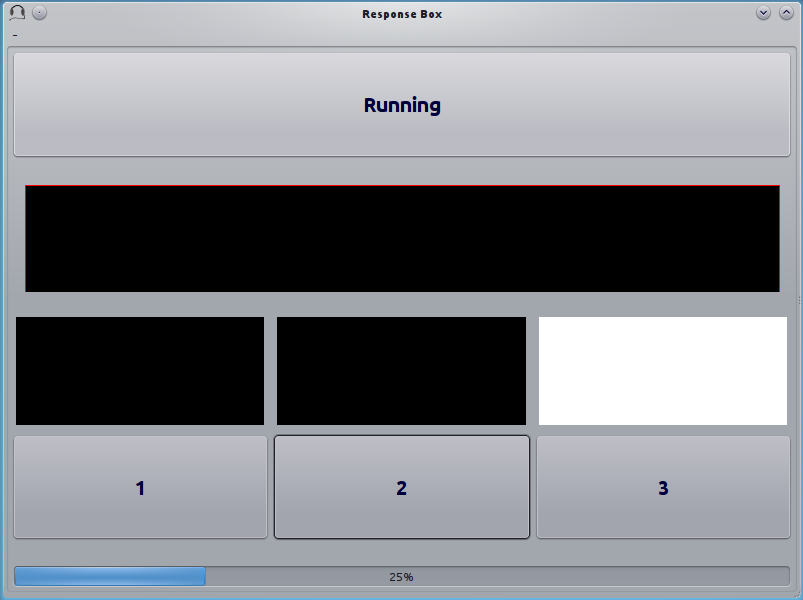
\includegraphics{response_box.png}}
\caption{The pychoacoustics response box}\label{intro:fig-response-box}\end{figure}
\begin{figure}[htbp]
\centering
\capstart

\scalebox{0.500000}{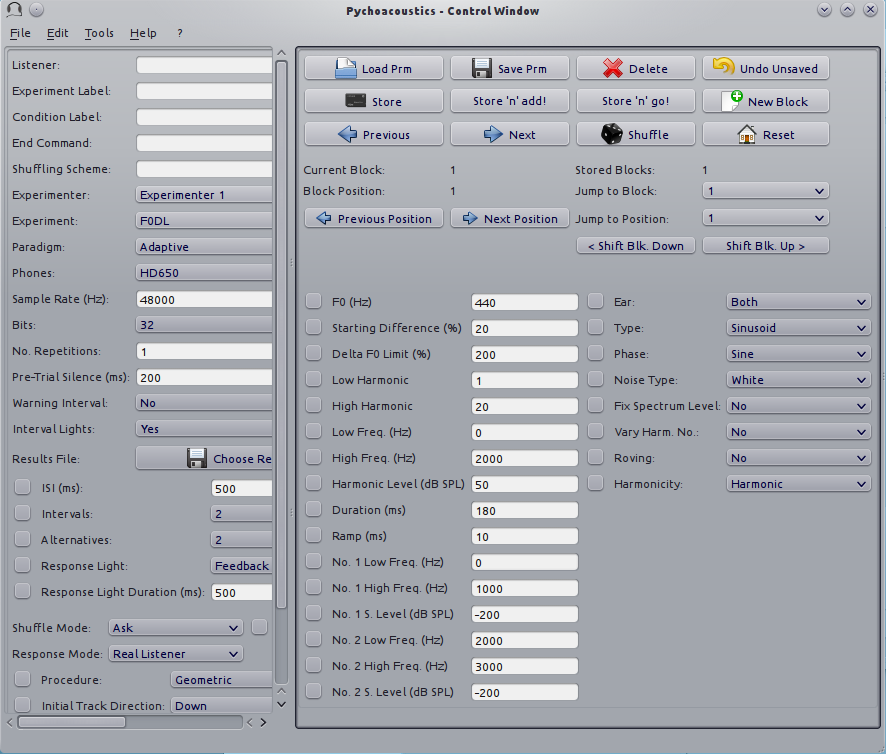
\includegraphics{control_window.png}}
\caption{The pychoacoustics control window}\label{intro:fig-control-window}\end{figure}

I started writing \code{pychoacoustics} for fun and for the sake of
learning around 2008 while doing my PhD with Professor Chris Plack at
Lancaster University. At that time we were using in the lab a MATLAB
program called the “Earlab” written by Professor Plack.
\code{pychoacoustics} has been greatly influenced and inspired by the
“Earlab”. For this reason, as well as for the patience he had to teach
me audio programming, I am greatly indebted to Professor Plack.


\chapter{Installation}
\label{installation:sec-installation}\label{installation:installation}\label{installation::doc}
\code{pychoacoustics} has been successfully installed and used on Linux and
Windows platforms. Given that it is entirely written in Python, it should be
fully cross-platform and should work on the Mac as well, but this has
never been tested. \code{pychoacoustics} depends on the installation of a
handful of other programs:
\begin{itemize}
\item {} 
Python (version 3) \href{http://www.python.org/}{http://www.python.org/}

\item {} 
pyqt4
\href{http://www.riverbankcomputing.co.uk/software/pyqt/download}{http://www.riverbankcomputing.co.uk/software/pyqt/download}

\item {} 
numpy
\href{http://sourceforge.net/projects/numpy/files/}{http://sourceforge.net/projects/numpy/files/}

\item {} 
scipy
\href{http://sourceforge.net/projects/scipy/files/}{http://sourceforge.net/projects/scipy/files/}

\end{itemize}

these programs need to be installed manually. Once these programs are
installed you can proceed with the installtion of \code{pychoacoustics}.


\section{Installation on Linux}
\label{installation:installation-on-linux}
Binary deb packages for recent debian-based distributions are provided
(starting from Wheezy), and can be installed using gdebi which
automatically handles dependencies. For other linux systems, once all of
the dependencies have been installed, \code{pychoacoustics} can be
installed as a standard python package using

\begin{Verbatim}[commandchars=\\\{\}]
sudo python3 setup.py install
\end{Verbatim}

you can then invoke \code{pychoacoustics} from a terminal by typing the
command

\begin{Verbatim}[commandchars=\\\{\}]
\PYG{n}{pychoacoustics}\PYG{o}{.}\PYG{n}{pyw}
\end{Verbatim}


\section{Installation on Windows}
\label{installation:installation-on-windows}

\subsection{Using the binary installer}
\label{installation:using-the-binary-installer}
After installing the dependencies (\code{python}, \code{pyqt4}, \code{numpy}, and
\code{scipy}), simply double click on the \code{pychoacoustics} windows
installer to start the installation procedure. Currently the installer
does not provide an application launcher. There is, however, a file called
\code{pychoacoustics-qt4.bat} inside the source distribution of
pychoacoustics that after some modifications can be used as a launcher.
The content of the file is the following:

\begin{Verbatim}[commandchars=\\\{\}]
C:\PYGZbs{}Python32\PYGZbs{}python "C:\PYGZbs{}Python32\PYGZbs{}site-packages\PYGZbs{}pychoacoustics.pyw"
\%1 \%2 \%3 \%4 \%5 \%6 \%7 \%8
\end{Verbatim}

The first statement \code{C:\textbackslash{}Python32\textbackslash{}python} is the path to the Python
executable. The second statement is the path to the main file of the
\code{pychoacoustics} app. You simply need to replace those two statements
to reflect the Python installation on your system. You can place the \code{.bat} launcher wherever you want, for example on your \code{Desktop} folder. Simply double click on it, and \code{pychoacoustics} should start.


\subsection{Installing from source}
\label{installation:installing-from-source}
After installing the dependencies, it is recommended to add the
directory where the Python executable resides to the system \code{PATH}. In
this way you can call \code{python} from a \code{DOS} shell by simply typing
its name, rather than typing the full path to the Python executable.

By default \code{python} is installed in \code{C:}. The name of the Python
directory depends on its version number, for example, if you installed
Python version 3.2, the python directory will be \code{C:\textbackslash{}Python32}. To add
this directory to the system path go to \code{My Computer} and click
\code{Properties}, then click \code{Advanced System Settings}. In the
\code{System Properties} window click \code{Environment Variables}. There you
will find an entry called \code{Path}. Select it and click \code{Edit}. Be
careful not to remove any of the entries that are already written there
because it could corrupt your system. Simply append the name of the full
path of the folder where Python is installed, at the end of the
other entries.

To install \code{pychoacoustics} from source, unpack the \code{pychoacoustics}
\code{.zip} file containing the source code. Open a \code{DOS} shell and
\code{cd} to the directory where you unzipped pychoacoustics. The program
can then be installed as a standard python package using the following
command:

\begin{Verbatim}[commandchars=\\\{\}]
python setup.py install
\end{Verbatim}

If you have installed the dependencies, you can also use pychoacoustics
without installing it. Open a \code{DOS} shell, \code{cd} to the directory
where you unzipped pychoacoustics and launch it with the following
command:

\begin{Verbatim}[commandchars=\\\{\}]
python pychoacoustics.pyw
\end{Verbatim}

As mentioned in the previous section, there is also a \code{.bat} launcher
that can be used to launch \code{pychoacoustics} without needing to open a
\code{DOS} shell each time. You can read the previous section for further
info.


\chapter{Graphical User Interface}
\label{graphical_user_interface:sec-graphical-user-interface}\label{graphical_user_interface::doc}\label{graphical_user_interface:graphical-user-interface}
The user interface is divided into two windows: the “Control Window” and
the “Response Box”. The “Control Window” is used to set the experimental
parameters, while the “Response Box” is the interface that the listeners
use to give their responses.


\section{Quickstart}
\label{graphical_user_interface:quickstart}
When \code{pychoacoustics} is launched, the “Control Window” displays the
default parameters for the “Audiogram” experiment. You can select
another experiment using the “Experiment” drop-down menu, and edit any
of the parameter fields you want to modify. Once you’re satisfied with
the parameters, you can store them by pressing the “Store” button. This
stores one experimental block with the chosen parameters. At this point
you can either start running the experiment by pressing the “Start”
button on the “Response Box”, or you can add more experimental blocks by
clicking on the “New Block” button.

To save the parameters to a file click on the “Save Prm” button.
Parameter files that have been saved in this way can be later loaded
into the program by using the “Load Prm” button.

To save the results of your experiment to a file, click on the “Save
Results” button. If you have forgotten to specify a results file in this
way, \code{pychoacoustics} will save the results in a file called
\code{test.txt} in the working directory.


\section{The Control Window}
\label{graphical_user_interface:the-control-window}
The control window contains a set of widgets to manage the setup of the
experiments, running the experiments, processing results files and
managing application preferences. Some of the widgets are general, and
some of them are specific either to a given paradigm (e.g. adaptive vs
constant stimuli paradigm) or to a given experiment.

In the next section the function of these widgets will be explained,
starting with the widgets that are general to all experiments and
paradigms.


\subsection{General Widgets (left panel)}
\label{graphical_user_interface:general-widgets-left-panel}\label{graphical_user_interface:sec-gui-left-panel}\begin{itemize}
\item {} 
\textbf{Listener} This is simply a label that you can use to identify the
person who is running the experiment. This label will be written in
the header of the results file.

\item {} 
\textbf{Experiment Label}. This is a label to identify the experiment you
are running. This label will be written in the header of the results
file.

\item {} 
\textbf{Session} This is a label to identify the experimental session, it
can be a number or a string. This label will be written in the header
of the results file.

\item {} 
\textbf{Condition Label} This is a label to identify the experimental
condition of the current block of trials. It is optional, but it may
be useful when sorting the experimental results.

\item {} 
\textbf{End Command} Here you can write an operating system command
(e.g. a bash command on Unix systems or a DOS command on Windows
systems) to be performed at the end of the experimental session. This
could be used to run a custom script to analyse the result files,
make a backup of the results files or other purposes. There are some
variables that can be accessed with a special string, such as the
name of the results file. These are listed in
Section {\hyperref[engine:sec-os-commands]{\emph{OS Commands}}} Table {\hyperref[engine:tab-pycho-variables]{\emph{pychoacoustics variables}}}
Please, refer to that section for further info on how to use them.

\item {} 
\textbf{Shuffling Scheme} By default when you click the “Shuffle” button,
\code{pychoacoustics} randomly shuffles all blocks, here you can specify
different shuffling schemes (e.g. shuffle the first four blocks among
themselves and the last four blocks among themselves). Please refer
to Section {\hyperref[engine:sec-shuffling]{\emph{Block Presentation Position}}} for more details.

\item {} 
\textbf{Results File} Select a file for saving the results. Selecting an
existing file will never overwrite its content, it will simply append
the new results to its content. If no file is selected, the results
will be saved in a file called \code{test.txt} in the current working
directory. You can select a file to save the results even after you
have started a block of trials, the results get written to the file
only at the end of the block.

\item {} 
\textbf{Experimenter} Here you can select one of the experimenters listed
in the experimenter database. Please refer to
Section {\hyperref[graphical_user_interface:sec-edit-experimenters-dia]{\emph{Edit Experimenters Dialog}}} for further info on the
experimenter database and how it can be used.

\item {} 
\textbf{Experiment} Selects the experiment for the current block.

\item {} 
\textbf{Paradigm} Selects the paradigm (e.g. adaptive, constant, etc…) for
the current block. The list of paradigms available depends on the
experiment that is selected.

\item {} 
\textbf{Phones} Choose from one of the phone models stored in the phones
database. Please, refer to Section {\hyperref[graphical_user_interface:sec-edit-phones-dia]{\emph{Edit Phones Dialog}}} for
further info on how to enter phones and calibration values in the
database.

\item {} 
\textbf{Sample Rate (Hz)} Set the sampling rate of the sounds to be
played. Any value can be entered in the text fields. However, you
should enter a value that is supported by your soundcard. A value
that is not supported by your souncard may lead to issues, although
it’s more likely that your soundcard will perform an automatic sample
rate conversion.

\item {} 
\textbf{Bits} Set the bit depth that \code{pychoacoustics} uses to store
sounds to a wav file or play them. Currently values of 16 and 32 bits
are supported. A value of 32 bits can be used for 24-bit soundcards.
Notice that to achieve 24-bit output requires both a 24-bit souncard
and a play command that can output 24-bit sounds. Therefore selecting
a value of 32 bits here does not guarantee 24-bit playback even if
you have a 24-bit souncard. Please, refere to
Section {\hyperref[engine:sec-sound-output]{\emph{Sound Output}}} for further information on this
issue.

\item {} 
\textbf{Repetitions} Set the number of times the sequence of blocks stored
in memory should be repeated. If the “Shuffle Mode” (see below) is
set to “auto”, each time a new repetition starts the block positions
will be shuffled. If the “Shuffle Mode” is set to “Ask”, each time a
new repetition starts the user will be asked if s/he wants to shuffle
the block positions. The “Reset” button resets the number of
repetitions to zero.

\item {} 
\textbf{Pre-Trial Silence (ms)} Set a silent time interval before the
start of each trial.

\item {} 
\textbf{Warning Interval} Choose whether to present a warning light at the
beginning of each trial.

\item {} 
\textbf{Warning Interval Duration (ms)} Sets the duration of the warning
interval light. This widget is shown only if the warning interval
chooser is set to “Yes”.

\item {} 
\textbf{Warning Interval ISI (ms)} Sets the duration of the silent
interval between the end of warning interval and the start of the
first observation interval. This widget is shown only if the warning
interval chooser is set to “Yes”.

\item {} 
\textbf{Pre-Trial Interval} Choose whether to present a pre-trial
interval. This widget is shown only for experiments that have a
pre-trial interval option.

\item {} 
\textbf{Pre-Trial Interval ISI (ms)} Sets the duration of the silent
interval between the end of pre-trial interval and the start of the
first observation interval. This widget is shown only if the current
experiment has a pre-trial interval option and the pre-trial interval
chooser is set to “Yes”.

\item {} 
\textbf{Response Light} Set the type of response light at the end of each
trial. ``Feedback'' will flash a green (correct response) or red
(incorrect response) light. ``Neutral'' will flash a white light.
``None'' will not flash any light (there will nonetheless be a silent
interval equal to the response light duration, see below).

\item {} 
\textbf{Response Light Duration (ms)} Set the duration of the response
light.

\item {} 
\textbf{Shuffle Mode} If the “Shuffle Mode” is “auto”, the block
presentation positions will be automatically shuffled at the
beginning of a series of blocks. If the “Shuffle Mode” is “Ask”, at
the beginning of a series of blocks the user will be asked if the
block presentation positions should be shuffled or not. If the
“Shuffle Mode” is “No”, the block presentation positions will not be
automatically shuffled at the beginning of a series of blocks. See
Section {\hyperref[engine:sec-shuffling]{\emph{Block Presentation Position}}} for further information on shuffling the
block presentation positions.

\item {} 
\textbf{Response Mode} When “Real Listener” is selected,
\code{pychoacoustics} waits for responses from a human listener. When
“Automatic” is selected the program will give responses by itself
with a certain percentage correct, that can be specified in the
“Percent Correct (\%)” text field. This mode is mostly useful for
debugging purposes, however it can also be used for experiments in
which the participants are passively listening to the stimuli (e.g.
some neuroimaging experiments that record cerebral responses rather
than behavioural responses). In “Simulated Listener” mode
\code{pychoacoustics} will give responses on the bases of an auditory
model. This model needs to be specified in the experiment file, the
“Simulated Listener” mode provides just a hook to redirect the
control flow to your model. Please, refer to
Section {\hyperref[engine:sec-response-mode]{\emph{Response Mode}}} for more information.

\end{itemize}


\subsection{General Widgets (right panel)}
\label{graphical_user_interface:general-widgets-right-panel}\begin{itemize}
\item {} 
\textbf{Load Prm} Load in memory experimental parameters stored in a
\code{.prm} file. See Section {\hyperref[engine:sec-parameters-files]{\emph{Parameters Files}}} for more
info.

\item {} 
\textbf{Save Prm} Save experimental parameters stored in memory in a
\code{.prm} file. See Section {\hyperref[engine:sec-parameters-files]{\emph{Parameters Files}}} for more
info.

\item {} 
\textbf{Delete} Delete the current block from the blocks list.

\item {} 
\textbf{Undo Unsaved} Reset the parameters in the current block to the
parameters that were last saved.

\item {} 
\textbf{Store} Store the parameters changes in memory.

\item {} 
\textbf{Store ’n’ add} Store the parameter changes in memory and add a new
parameters block.

\item {} 
\textbf{Store ’n’ go} Store the parameter changes in memory and move to
the next block storage point.

\item {} 
\textbf{New Block} Create a new parameters block (the parameters of the
current block will be copied in the new one).

\item {} 
\textbf{Previous} Move to the previous block storage point.

\item {} 
\textbf{Next} Move to the next block storage point.

\item {} 
\textbf{Shuffle} Shuffle the block presentation positions.

\item {} 
\textbf{Reset} Reset the block presentation positions and move to the
first block position.

\item {} 
\textbf{Jump to Block} Jump to a given block storage point.

\item {} 
\textbf{Previous Position} Move to the previous block presentation
position.

\item {} 
\textbf{Next Position} Move to the next block presentation position.

\item {} 
\textbf{Jump to Position} Jump to the given block presentation position.

\item {} 
\textbf{Shift Blk. Down} Shift the current block to a lower storage point.

\item {} 
\textbf{Shift Blk. Up} Shift the current block to a higher storage point.

\end{itemize}


\subsection{Paradigm Widgets}
\label{graphical_user_interface:paradigm-widgets}

\subsubsection{Adaptive Paradigm Widgets}
\label{graphical_user_interface:adaptive-paradigm-widgets}\begin{itemize}
\item {} 
\textbf{Procedure} If “Arithmetic” the quantity defined by the step size
will be added or subtracted to the parameter that is adaptively
changing. If “Geometric” the parameter that is adaptively changing
will be multiplied or divided by the quantity defined by the step
size.

\item {} 
\textbf{Initial Track Direction} This determines when the first turpoint
will be called. If the initial track direction is “Down” the first
turnpoint will be called the first time the adaptive track turns
upward. If the initial track direction is “Up” the first turnpoint
will be called the first time the adaptive track turns downward.

\item {} 
\textbf{Rule Down} Set the number of consecutive correct responses needed
to subtract the current step size from the adaptive parameter (for
arithmetic procedures) or divide the adaptive parameter by the
current step size (for geometric procedures).

\item {} 
\textbf{Rule Up} Set the number of consecutive incorrect responses needed
to add the current step size to the adaptive parameter (for
arithmetic procedures) or multiply the adaptive parameter by the
current step size (for geometric procedures).

\item {} 
\textbf{Initial Turnpoints} Set the number of initial turnpoints. The
initial turnpoints serve to bring quickly the adaptive track towards
the listener’s threshold. These turnpoints are not included in the
threshold estimate.

\item {} 
\textbf{Total Turnpoints} Set the number of total turnpoints. The number
of total turnpoints is equal to the number of initial turnpoints that
are not included in the threshold estimate plus the number of
turnpoints that you want to use for the threshold estimate.

\item {} 
\textbf{Step Size 1} Set the step size for the initial turnpoints.

\item {} 
\textbf{Step Size 2} Set the step size to be used after the number of
initial turnpoints has been reached.

\end{itemize}


\subsubsection{Weighted Up/Down Paradigm Widgets}
\label{graphical_user_interface:weighted-up-down-paradigm-widgets}\begin{itemize}
\item {} 
\textbf{Procedure} If “Arithmetic” the quantity defined by the step size
will be added or subtracted to the parameter that is adaptively
changing. If “Geometric” the parameter that is adaptively changing
will be multiplied or divided by the quantity defined by the step
size.

\item {} 
\textbf{Initial Track Direction} This determines when the first turpoint
will be called. If the initial track direction is “Down” the first
turnpoint will be called the first time the adaptive track turns
upward. If the initial track direction is “Up” the first turnpoint
will be called the first time the adaptive track turns downward.

\item {} 
\textbf{Percent Correct Tracked} Set the percentage correct point on the
psychometric function to be tracked by the adaptive procedure. The
ratio of the “Up” and “Down” steps is automatically adjusted by the
software to satisfy this criterion.

\item {} 
\textbf{Initial Turnpoints} Set the number of initial turnpoints. The
initial turnpoints serve to bring quickly the adaptive track towards
the listener’s threshold. These turnpoints are not included in the
threshold estimate.

\item {} 
\textbf{Total Turnpoints} Set the number of total turnpoints. The number
of total turnpoints is equal to the number of initial turnpoints that
are not included in the threshold estimate plus the number of
turnpoints that you want to use for the threshold estimate.

\item {} 
\textbf{Step Size 1} Set the “Down” step size for the initial turnpoints.
The “Up” step size is automatically calculated to satisfy the
“Percent Correct Tracked” criterion.

\item {} 
\textbf{Step Size 2} Set the “Down” step size to be used after the number
of initial turnpoints has been reached. The “Up” step size is
automatically calculated to satisfy the “Percent Correct Tracked”
criterion.

\end{itemize}


\subsubsection{Adaptive Interleaved Paradigm Widgets}
\label{graphical_user_interface:adaptive-interleaved-paradigm-widgets}\begin{itemize}
\item {} 
\textbf{Procedure} If “Arithmetic” the quantity defined by the step size
will be added or subtracted to the parameter that is adaptively
changing. If “Geometric” the parameter that is adaptively changing
will be multiplied or divided by the quantity defined by the step
size.

\item {} 
\textbf{No. Tracks} Set the number of adaptive tracks.

\item {} 
\textbf{Max. Consecutive Trials x Track} Set the maximum number of
consecutive trials per track.

\item {} 
\textbf{Turnpoints to Average} Since track selection is pseudo-random, it
may happen that for a track the number of total turnpoints collected
is greater than the number of total turnpoints requested for that
track. If “All final step size (even)” is selected, the threshold
will be estimated using all the turnpoints collected after the
initial turnpoints, unless the number of these turnpoints is odd, in
which case the first of these turnpoints will be discarded. If “First
N final step size” is selected the threshold will be estimated using
only the number of requested turnpoints collected after the initial
turnpoints. If “Last N final step size” is selected the threshold
will be estimated using only the last $N$ turnpoints, where
$N$ equals the number of requested turnpoints.

\item {} 
\textbf{Initial Track X Direction} This determines when the first turpoint
will be called for track number $X$. If the initial track
direction is “Down” the first turnpoint will be called the first time
the adaptive track turns upward. If the initial track direction is
“Up” the first turnpoint will be called the first time the adaptive
track turns downward.

\item {} 
\textbf{Rule Down Track X} Set the number of consecutive correct responses
needed to subtract the current step size from the adaptive parameter
(for arithmetic procedures) or divide the adaptive parameter by the
current step size (for geometric procedures) for track number
$X$.

\item {} 
\textbf{Rule Up Track X} Set the number of consecutive incorrect responses
needed to add the current step size to the adaptive parameter (for
arithmetic procedures) or multiply the adaptive parameter by the
current step size (for geometric procedures) for track number
$X$.

\item {} 
\textbf{Initial Turnpoints Track X} Set the number of initial turnpoints
for track number $X$. The initial turnpoints serve to bring
quickly the adaptive track towards the listener’s threshold. These
turnpoints are not included in the threshold estimate.

\item {} 
\textbf{Total Turnpoints Track X} Set the number of total turnpoints for
track number $X$. The number of total turnpoints is equal to
the number of initial turnpoints that are not included in the
threshold estimate plus the number of turnpoints that you want to use
for the threshold estimate.

\item {} 
\textbf{Step Size 1 Track X} Set the step size for the initial turnpoints
for track number $X$.

\item {} 
\textbf{Step Size 2 Track X} Set the step size to be used after the number
of initial turnpoints has been reached for track number $X$.

\end{itemize}


\subsubsection{Weighted Up/Down Interleaved Paradigm Widgets}
\label{graphical_user_interface:weighted-up-down-interleaved-paradigm-widgets}\begin{itemize}
\item {} 
\textbf{Procedure} If “Arithmetic” the quantity defined by the step size
will be added or subtracted to the parameter that is adaptively
changing. If “Geometric” the parameter that is adaptively changing
will be multiplied or divided by the quantity defined by the step
size.

\item {} 
\textbf{No. Tracks} Set the number of adaptive tracks.

\item {} 
\textbf{Max. Consecutive Trials x Track} Set the maximum number of
consecutive trials per track.

\item {} 
\textbf{Turnpoints to Average} Since track selection is pseudo-random, it
may happen that for a track the number of total turnpoints collected
is greater than the number of total turnpoints requested for that
track. If “All final step size (even)” is selected, the threshold
will be estimated using all the turnpoints collected after the
initial turnpoints, unless the number of these turnpoints is odd, in
which case the first of these turnpoints will be discarded. If “First
N final step size” is selected the threshold will be estimated using
only the number of requested turnpoints collected after the initial
turnpoints. If “Last N final step size” is selected the threshold
will be estimated using only the last $N$ turnpoints, where
$N$ equals the number of requested turnpoints.

\item {} 
\textbf{Initial Track X Direction} This determines when the first turpoint
will be called for track number $X$. If the initial track
direction is “Down” the first turnpoint will be called the first time
the adaptive track turns upward. If the initial track direction is
“Up” the first turnpoint will be called the first time the adaptive
track turns downward.

\item {} 
\textbf{Percent Correct Tracked} Set the percentage correct point on the
psychometric function to be tracked by the adaptive procedure for
track number $X$. The ratio of the “Up” and “Down” steps is
automatically adjusted by the software to satisfy this criterion.

\item {} 
\textbf{Initial Turnpoints Track X} Set the number of initial turnpoints
for track number $X$. The initial turnpoints serve to bring
quickly the adaptive track towards the listener’s threshold. These
turnpoints are not included in the threshold estimate.

\item {} 
\textbf{Total Turnpoints Track X} Set the number of total turnpoints for
track number $X$. The number of total turnpoints is equal to
the number of initial turnpoints that are not included in the
threshold estimate plus the number of turnpoints that you want to use
for the threshold estimate.

\item {} 
\textbf{Step Size 1 Track X} Set the “Down” step size for the initial
turnpoints for track number $X$. The “Up” step size is
automatically calculated to satisfy the “Percent Correct Tracked”
criterion.

\item {} 
\textbf{Step Size 2 Track X} Set the “Down” step size to be used after the
number of initial turnpoints has been reached for track number
$X$. The “Up” step size is automatically calculated to satisfy
the “Percent Correct Tracked” criterion.

\end{itemize}


\subsubsection{Constant m-Intervals n-Alternatives Paradigm Widgets}
\label{graphical_user_interface:constant-m-intervals-n-alternatives-paradigm-widgets}\begin{itemize}
\item {} 
\textbf{No. Trials} Set the number of trials to be presented in the
current block.

\item {} 
\textbf{No. Practice Trials} Set the number of practice trials to be
presented in the current block. Practice trials are presented at the
beginning of the block; the responses to these trials are not
included in the statistics.

\end{itemize}


\subsubsection{Multiple Constants m-Intervals n-Alternatives Paradigm Widgets}
\label{graphical_user_interface:multiple-constants-m-intervals-n-alternatives-paradigm-widgets}\begin{itemize}
\item {} 
\textbf{No. Trials} Set the number of trials to be presented in the
current block for each condition.

\item {} 
\textbf{No. Practice Trials} Set the number of practice trials to be
presented in the current block for each condition. The responses to
these trials are not included in the statistics.

\item {} 
\textbf{No. Differences} Set the number of conditions to be used in the
current block.

\end{itemize}


\subsubsection{Constant 1-Interval 2-Alternatives Paradigm Widgets}
\label{graphical_user_interface:constant-1-interval-2-alternatives-paradigm-widgets}\begin{itemize}
\item {} 
\textbf{No. Trials} Set the number of trials to be presented in the
current block.

\item {} 
\textbf{No. Practice Trials} Set the number of practice trials to be
presented in the current block. Practice trials are presented at the
beginning of the block; the responses to these trials are not
included in the statistics.

\end{itemize}


\subsubsection{Multiple Constants 1-Interval 2-Alternatives Paradigm Widgets}
\label{graphical_user_interface:multiple-constants-1-interval-2-alternatives-paradigm-widgets}\begin{itemize}
\item {} 
\textbf{No. Trials} Set the number of trials to be presented in the
current block for each condition.

\item {} 
\textbf{No. Practice Trials} Set the number of practice trials to be
presented in the current block for each condition. The responses to
these trials are not included in the statistics.

\item {} 
\textbf{No. Differences} Set the number of conditions to be used in the
current block.

\end{itemize}


\subsubsection{1-Pair Same/Different Paradigm Widgets}
\label{graphical_user_interface:pair-same-different-paradigm-widgets}\begin{itemize}
\item {} 
\textbf{No. Trials} Set the number of trials to be presented in the
current block.

\item {} 
\textbf{No. Practice Trials} Set the number of practice trials to be
presented in the current block. Practice trials are presented at the
beginning of the block; the responses to these trials are not
included in the statistics.

\end{itemize}


\subsection{The Menu Bar}
\label{graphical_user_interface:the-menu-bar}
A screenshot of the menu bar is shown in Figure {\hyperref[graphical_user_interface:fig-menu-bar]{\emph{The menu bar}}}. This bar
is located in the upper left corner of the “Control Window”. Each menu
will be described below.
\begin{figure}[htbp]
\centering
\capstart

\scalebox{1.000000}{
\includegraphics{menuBar.png}}
\caption{The menu bar}\label{graphical_user_interface:fig-menu-bar}\end{figure}


\subsubsection{The File Menu}
\label{graphical_user_interface:the-file-menu}\begin{itemize}
\item {} 
\textbf{Process Results} Process block summary results files to obtain
session summary results files. For more info see
Section {\hyperref[graphical_user_interface:sec-process-results-dialog]{\emph{Process Results Dialog}}}.

\item {} 
\textbf{Process Results Table} Process block summary results table files
to obtain session summary table results files. For more info see
Section  {\hyperref[graphical_user_interface:sec-process-results-dialog]{\emph{Process Results Dialog}}}.

\item {} 
\textbf{Open Results File} Open the file where \code{pychoacoustics} is
currently saving data with the default text editor.

\item {} 
\textbf{Exit.} Close \code{pychoacoustics}.

\end{itemize}


\subsubsection{The Edit Menu}
\label{graphical_user_interface:the-edit-menu}\begin{itemize}
\item {} 
\textbf{Edit Preferences} Edit application preferences. See
Section {\hyperref[graphical_user_interface:sec-edit-preferences-dia]{\emph{Edit Preferences Dialog}}} for further info.

\item {} 
\textbf{Edit Phones} Edit the phones database, and set the calibration
levels for your phones. See Section {\hyperref[graphical_user_interface:sec-edit-phones-dia]{\emph{Edit Phones Dialog}}} for
further info.

\item {} 
\textbf{Edit Experimenters} Edit the experimenters database. See
Section {\hyperref[graphical_user_interface:sec-edit-experimenters-dia]{\emph{Edit Experimenters Dialog}}} for further info.

\end{itemize}


\subsubsection{The Tools Menu}
\label{graphical_user_interface:the-tools-menu}\begin{itemize}
\item {} 
\textbf{Swap Blocks} Swap the storage position of two parameter blocks.

\end{itemize}


\subsubsection{The Help Menu}
\label{graphical_user_interface:the-help-menu}\begin{itemize}
\item {} 
\textbf{Fortunes} Show psychoacoustics fortunes. I’m always collecting new
ones, so if you happen to know any interesting ones, please, e-mail
them to me so that I can add them to the collection.

\item {} 
\textbf{About pychoacoustics} Show information about the licence, the
version of the software and the version of the libraries it depends
on.

\end{itemize}


\subsubsection{The “what’s this?” Button.}
\label{graphical_user_interface:the-whats-this-button}
If you click on this button, and then click on a widget, you can get
some information about the widget (this is not implemented for all
widgets).


\section{Process Results Dialog}
\label{graphical_user_interface:process-results-dialog}\label{graphical_user_interface:sec-process-results-dialog}
Figure {\hyperref[graphical_user_interface:fig-proc-res-dia]{\emph{The process results dialog}}} show a screenshot of the
process results dialog. The dialog is the same for all procedures,
except that for procedures in which \emph{d’} is computed, there is an
additional checkbox asking whether to apply a correction to hit/false
alarm rates of zero or one. For information on the format of the result
files, please see Section {\hyperref[engine:sec-results-files]{\emph{Results Files}}}.
\begin{figure}[htbp]
\centering
\capstart

\scalebox{1.000000}{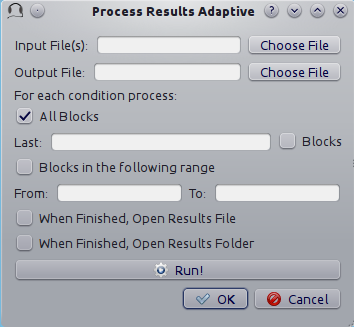
\includegraphics{proc_res_dia.png}}
\caption{The process results dialog}\label{graphical_user_interface:fig-proc-res-dia}\end{figure}
\begin{itemize}
\item {} 
\textbf{Input File(s)} Give the filepath of one or more files to be
processed. The “Choose File” button can be used to select the
file(s). Multiple filepaths should be separated by a semicolon
“\code{;}”.

\item {} 
\textbf{Output File} Give the filename of the output file.

\item {} 
\textbf{For each condition process:}
\begin{itemize}
\item {} 
\textbf{All Blocks} If checked, all blocks in the result file(s) will
be processd.

\item {} 
\textbf{Last X Blocks} If checked, only the last $X$ blocks will
be processed.

\item {} 
\textbf{Blocks in the following range} If checked, only blocks in the
specified range will be processed (indexing starts from 1).

\end{itemize}

\item {} 
\textbf{d-prime correction} If checked, convert hit rates of $0$ and
$1$ to $1/2N$ and $1-1/(2N)$ respectively, where
$N$ is the number of trials, to avoid infinite values of \emph{d’}
(see {\hyperref[references:macmillanandcreelman2005]{{[}MacmillanAndCreelman2005{]}}} p. 8). This checkbox is available only for some
paradigms.

\item {} 
\textbf{When finished, open results file} If checked, the output file will
be opened in the default text editor when processing has finished.

\item {} 
\textbf{When finished, open results folder} If checked, the folder
containing the output file will be opened when processing has
finished.

\item {} 
\textbf{Run!} Click this button to process the result files.

\end{itemize}


\section{Edit Preferences Dialog}
\label{graphical_user_interface:sec-edit-preferences-dia}\label{graphical_user_interface:edit-preferences-dialog}\begin{quote}

The preferences dialog is divided into several tabs. These are described in turn below.
\end{quote}


\subsection{General}
\label{graphical_user_interface:general}\label{graphical_user_interface:sec-edit-pref-dia-gen}\begin{itemize}
\item {} 
\textbf{Language (requires restart)} Choose the application language. At
the moment and for the foreseeable future only English is supported.

\item {} 
\textbf{Country (requires restart)} Set the country locale to be used for
the application. Some things (e.g. the way dates are written in
result files depend on this setting.

\item {} 
\textbf{Response Box Language (requires restart)} Choose the language to
be used for the “Response Box”. This set the language to be used for
the button labels and other GUI elements that the experimental
listener is presented with.

\item {} 
\textbf{Response Box Country (requires restart)} Set the country locale
for the response box.

\item {} 
\textbf{csv separator} Choose the separator field to be used when writing
the csv tabular result files.

\item {} 
\textbf{Warn if listener name missing} If checked, pop up a warning
message if the listener name is missing at the beginning of a
session.

\item {} 
\textbf{Warning if session label missing} If checked, pop up a warning
message if the session label is missing at the beginning of a
session.

\item {} 
\textbf{Process results when finished} If checked, process automatically
the block summary file to generate the session summary file at the
end of the experiment.

\item {} 
\textbf{d-prime correction} If checked, when automatically processing
result files, convert hit rates of $0$ and $1$ to
$1/2N$ and $1-1/(2N)$ respectively, where $N$ is
the number of trials, to avoid infinite values of \emph{d’}
(see {\hyperref[references:macmillanandcreelman2005]{{[}MacmillanAndCreelman2005{]}}} p. 8).

\item {} 
\textbf{Max Recursion Depth (requires restart)} Set the maximum recursion
depth of the Python interpreter stack. This setting should be changed
only if you intend to run \code{pychoacoustics} in automatic or
simulated listener response mode. Beware, setting a max recursion
depth value smaller than the default value may cause
\code{pychoacoustics} to crash or not even start. In case
\code{pychoacoustics} does not start because of this, delete your
preferences settings file to restore the default max recursion depth
value.

\end{itemize}


\subsection{Sound}
\label{graphical_user_interface:sound}\label{graphical_user_interface:sec-edit-pref-dia-sound}\begin{itemize}
\item {} 
\textbf{Play Command} Set an internal or external command to play sounds.

\item {} 
\textbf{Device} Set the soundcard to be used to play sounds. This chooser
is available only for certain internal play commands (currently
alsaaudio and pyaudio).

\item {} 
\textbf{Buffer Size (samples)} Set the buffer size in number of samples to
be used to output sounds. This chooser is available only for certain
internal play commands (currently alsaaudio and pyaudio).

\item {} 
\textbf{Default Sampling Rate} Set the default sampling rate.

\item {} 
\textbf{Default Bits} Set the default bit depth.

\item {} 
\textbf{Wav manager (requires restart)} Choose the wav manager.

\item {} 
\textbf{Write wav file} Write wav files with the sounds played on each
trial in the current \code{pychoacoustics} working directory.

\item {} 
\textbf{Write sound sequence segment wavs} For sound sequences, write a
wav file for each segment of the sequence in the current
\code{pychoacoustics} working directory.

\item {} 
\textbf{Append silence to each sound (ms)} Append a silence of the given
duration at the end of each sound. This is useful on some versions of
the Windows operating system that may cut the sound buffer before it
has ended resulting in audible clicks.

\end{itemize}


\subsection{Notifications}
\label{graphical_user_interface:notifications}\label{graphical_user_interface:sec-edit-pref-dia-notifications}\begin{itemize}
\item {} 
\textbf{Play End Message} If checked, play a wav file at the end of the
experiment. This could be short message to let the listeners know
they have finished and thank them for their participation in the
experiment. One or more wav files need to be set through the “Choose
wav” button for this work.

\item {} 
\textbf{Choose wav} Choose the wav file to be played as the end message.
Clicking on this button brings up another dialog where you can select
the wav files to be played and their output RMS. Only one of the wav
files listed here and with the “Use” flag set to will be randomly
chosen and played.

\item {} 
\textbf{blocks before end of experiment} Set how many blocks before the
end of the experiment the two actions listed below (send notification
e-mail and execute custom command) should be performed.

\item {} 
\textbf{Send notification e-mail} If checked, send a notification e-mail
to the experimenter to notify her that the experiment is about to
finish.

\item {} 
\textbf{Execute custom command} If checked, execute an operating system
command before the end of the experiment. This command could be used
to automatically send an sms for example.

\item {} 
\textbf{Send data via e-mail} At the end of the experiment, send the
results file to the experimenter .

\item {} 
\textbf{Execute custom command} At the end of the experiment, execute an
operating system command.

\item {} 
\textbf{Outgoing Server (SMTP)} Set the name of the SMTP server to be used
by \code{pychoacoustics} to send e-mails.

\item {} 
\textbf{Port} Set the port number for the SMTP server.

\item {} 
\textbf{Security} Set the security protocol for network exchanges with the
SMTP server.

\item {} 
\textbf{Server requires identification} Check this if the SMTP server
requires identification.

\item {} 
\textbf{Username} Set the username for the SMTP server.

\item {} 
\textbf{Password} Set the password for the SMTP server.

\item {} 
\textbf{Send test e-mail} Send a test e-mail to check that the server
settings are OK.

\end{itemize}


\subsection{EEG}
\label{graphical_user_interface:sec-edit-pref-dia-eeg}\label{graphical_user_interface:eeg}\begin{itemize}
\item {} 
\textbf{ON Trigger} The ON trigger value (decimal).

\item {} 
\textbf{OFF Trigger} The OFF trigger value (decimal).

\item {} 
\textbf{Trigger Duration (ms)} The duration of the trigger in
milliseconds.

\end{itemize}


\section{Edit Phones Dialog}
\label{graphical_user_interface:sec-edit-phones-dia}\label{graphical_user_interface:edit-phones-dialog}\begin{quote}

A screenshot of the “Edit Phones” dialog is
\end{quote}

shown in Figure {\hyperref[graphical_user_interface:fig-phones-database]{\emph{Edit Phones Dialog}}}.
\begin{figure}[htbp]
\centering
\capstart

\scalebox{0.750000}{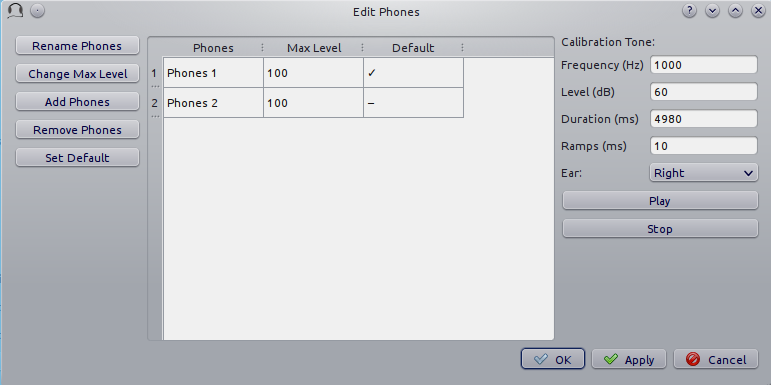
\includegraphics{phones_database.png}}
\caption{Edit Phones Dialog}\label{graphical_user_interface:fig-phones-database}\end{figure}

Most of the fields should be pretty much self-explanatory. Using this
dialog you can add headphones/earphones models to the phones database.
The phone with the “Default” flag set to will be selected by default
when \code{pychoacoustics} is started. In the “Max Level” field you should
enter the level in dB SPL that is output by the phone for a full
amplitude sinusoid. This value will be used by \code{pychoacoustics} to
output sounds at specific levels in dB SPL. On the rightmost panel of
the dialog you have facilities to play a sinusoid with a specified
level. You can use these facilities to check with a SPL meter (or a
voltmeter depending on how you’re doing it) that the actual output level
corresponds to the desired output level. Using these facilities you can
also play a full amplitude sinusoid: you need to set the level of the
sinuoid to the “Max Level” of the phone (whatever it is). Be careful
because it can be very loud!


\section{Edit Experimenters Dialog}
\label{graphical_user_interface:edit-experimenters-dialog}\label{graphical_user_interface:sec-edit-experimenters-dia}\begin{quote}

A screenshot of the “Edit
\end{quote}

Experimenters” dialog is shown in
Figure {\hyperref[graphical_user_interface:fig-experimenter-database]{\emph{Edit Experimenters Dialog}}}.
\begin{figure}[htbp]
\centering
\capstart

\scalebox{0.750000}{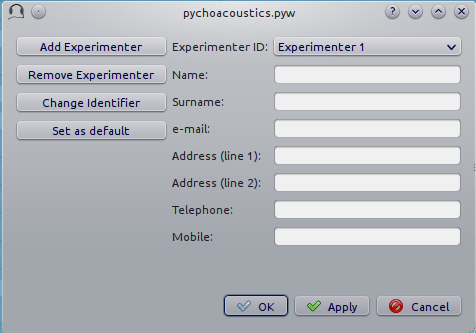
\includegraphics{experimenter_database.png}}
\caption{Edit Experimenters Dialog}\label{graphical_user_interface:fig-experimenter-database}\end{figure}

Most of the fields should be pretty much self-explanatory. Here you can
add the details of the experimenters that work in your lab in the
experimenter database. The main functions of this database at the moment
are a) writing the experimenter name in the results file; b) using the
experimenter e-mail for sending notifications and/or results files (see
Section {\hyperref[graphical_user_interface:sec-edit-pref-dia-notifications]{\emph{Notifications}}}).


\section{The Response Box}
\label{graphical_user_interface:the-response-box}
The “response box” consists of a large button (the “status button”) that
is used to start a block of trials, a feedback light to display trial by
trial feedback, interval lights to mark observation intervals, and
response buttons. The responses can be given either by means of mouse
clicks, or using the numeric keypad (key “1” for the first button, key
“2” for the second button etc…). Responses given before all observation
intervals have been presented are not accepted.

The status button can be activated by pressing the \code{Ctrl+R} shortcut.
At the start of each block the label of the “Status Button” is set to
“Start”. Once the listener starts a block of trials the label of the
status button changes to “Running”. When a whole series of blocks is
finished the label of the status button changes to “Finish”. If no
blocks are stored in memory the label of the status button is set to
“Wait”.

On the top left corner of the response box there is a semi-hidden menu
signalled by a little hyphen (“-”). If you click on it you have access
to two functions. The “Show/Hide Control Window” function can be used to
hide the control window while the experiment is running. This is useful
because it prevents the listener from accidentally changing your
experimental parameters or accidentally closing \code{pychoacoustics} (the
response box itself has no “close” button, so it is not possible to
close that). The “Show/Hide progress Bar” function can be used to
display a progress bar at the bottom of the response box. The progress
bar estimates what percentage of the experiment has been completed. This
estimate depends on the procedure used (for constant procedures it is
based on the number of trials done, while for adaptive procedures it is
based on the number of turnpoints reached) and on the specific
parameters of a given experiment (trial duration, number of trials, or
number or turnpoints, all of which can differ between blocks), so in
some cases the estimate can be off the mark. The “Show/Hide block
progress Bar” can be used to show the position of the current block and
the total number of blocks.


\chapter{Command Line User Interface}
\label{commandline_user_interface:sec-cmd-user-interface}\label{commandline_user_interface::doc}\label{commandline_user_interface:command-line-user-interface}
In order to automate certain tasks, or perform some advanced operations,
\code{pychoacoustics} can be called from the command line with a number of
command line options. The list of possible command line options is shown below:
\begin{itemize}
\item {} 
\code{-h, -{-}help} Show help message.

\item {} 
\code{-f, -{-}file FILE} Load parameters file \code{FILE}.

\item {} 
\code{-r, -{-}results FILE} Save the results to file \code{FILE}.

\item {} 
\code{-l, -{-}listener LISTENER} Set listener label to \code{LISTENER}.

\item {} 
\code{-s, -{-}session SESSION} Set session label to \code{SESSION}.

\item {} 
\code{-k, -{-}reset} Reset block positions.

\item {} 
\code{-q, -{-}quit} Quit after finished.

\item {} 
\code{-c, -{-}conceal} Hide Control and Parameters Windows.

\item {} 
\code{-p, -{-}progbar} Show the progress bar.

\item {} 
\code{-b, -{-}blockprogbar} Show the progress bar.

\item {} 
\code{-a, -{-}autostart} Automatically start the first stored block.

\item {} 
\code{-x, -{-}recursion-depth} Set the maximum recursion depth (this
overrides the maximum recursion depth set in the preferences window).

\item {} 
\code{-g, -{-}graphicssystem} sets the backend to be used for on-screen
widgets and QPixmaps. Available options are raster and opengl.

\item {} 
\code{-d, -{-}display} This option is only valid for X11 and sets the X
display (default is \$DISPLAY).

\end{itemize}

each command line option has a short (single dash, one letter) and long
(double dash, one word) form, for example to show the help message, you
can use either of the two following commands:

\begin{Verbatim}[commandchars=\\\{\}]
\$ pychoacoustics -h
\$ pychoacoustics --help
\end{Verbatim}


\chapter{Psychophysics}
\label{psychophysics:psychophysics}\label{psychophysics::doc}\label{psychophysics:sec-psychophysics}

\section{Available Paradigms}
\label{psychophysics:available-paradigms}\label{psychophysics:sec-paradigms}

\subsection{Adaptive}
\label{psychophysics:adaptive}
This paradigm implements the “up/down” adaptive procedures described by
{\hyperref[references:levitt1971]{{[}Levitt1971{]}}}. It can be used with $n$-intervals, $n$-alternatives forced
choice tasks, in which $n-1$ “standard” stimuli and a single
“comparison” stimulus are presented, each in a different temporal
interval. The order of the temporal intervals is randomized from trial
to trial. The “comparison” stimulus usually differs from the “standard”
stimuli for a single characteristic (e.g. pitch or loudness), and the
listener has to tell in which temporal interval it was presented. A
classical example is the 2-intervals 2-alternatives forced-choice task.
Tasks that present a reference stimulus in the first interval, and
therefore have $n$ intervals and $n-1$ alternatives are also
supported (see {\hyperref[references:grimaultetal2002]{{[}GrimaultEtAl2002{]}}} for an example of such tasks)


\subsection{Adaptive Interleaved}
\label{psychophysics:adaptive-interleaved}
This paradigm implements the interleaved adaptive procedure described by {\hyperref[references:jesteadt1980]{{[}Jesteadt1980{]}}} .


\subsection{Weighted Up/Down}
\label{psychophysics:weighted-up-down}
This paradigm implements the weighted up/down adaptive procedure
described by {\hyperref[references:kaernbach1991]{{[}Kaernbach1991{]}}}.


\subsection{Weighted Up/Down Interleaved}
\label{psychophysics:weighted-up-down-interleaved}
This paradigm combines the interleaved adaptive procedure described by {\hyperref[references:jesteadt1980]{{[}Jesteadt1980{]}}} with the weighted up/down method described by {\hyperref[references:kaernbach1991]{{[}Kaernbach1991{]}}}.


\subsection{Constant m-Intervals n-Alternatives}
\label{psychophysics:constant-m-intervals-n-alternatives}
This paradigm implements a constant difference method for forced choice
tasks with $m$-intervals and $n$-alternatives. For example,
it can be used for running a 2-intervals, 2-alternatives forced-choice
frequency-discrimination task with a constant difference between the
stimuli in the standard and comparison intervals.


\subsection{Constant 1-Interval 2-Alternatives}
\label{psychophysics:constant-1-interval-2-alternatives}
This paradigm implements a constant difference method for tasks with a
single observation interval and two response alternatives, such as the
“Yes/No” signal detection task.


\subsection{Constant 1-Pair Same/Different}
\label{psychophysics:constant-1-pair-same-different}
This paradigm implements a constant difference method for
“same/different” tasks with a single pair of stimuli to compare.


\chapter{Default Experiments}
\label{default_experiments:default-experiments}\label{default_experiments::doc}

\section{Audiogram}
\label{default_experiments:audiogram}\label{default_experiments:module-pychoacoustics.default_experiments.audiogram}\index{pychoacoustics.default\_experiments.audiogram (module)}
This experiment can be used to measure thresholds for detecting a signal in quiet.
The signal can be either a pure tone or a narrow-band noise.

The available fields are:
\begin{itemize}
\item {} \begin{description}
\item[{Frequency (Hz) :}] \leavevmode
Signal center frequency in Hz

\end{description}

\item {} \begin{description}
\item[{Bandwidth (Hz) :}] \leavevmode
The bandwidth of the signal in Hz (only applicable if
signal type is Narrowband Noise)

\end{description}

\item {} \begin{description}
\item[{Level (dB SPL) :}] \leavevmode
Signal level (for constant procedures), or starting signal level
(for adaptive procedures), in dB SPL

\end{description}

\item {} \begin{description}
\item[{Duration (ms) :}] \leavevmode
Signal duration (excluding ramps), in ms

\end{description}

\item {} \begin{description}
\item[{Ramps (ms) :}] \leavevmode
Duration of each ramp, in ms

\end{description}

\end{itemize}

The available choosers are:
\begin{itemize}
\item {} \begin{description}
\item[{Ear: {[}\code{Right}, \code{Left}, \code{Both}{]}}] \leavevmode
The ear to which the signal will be presented

\end{description}

\item {} \begin{description}
\item[{Signal Type: {[}\code{Sinusoid}, \code{Narrowband Noise}{]}}] \leavevmode
The signal type. If \code{Sinusoid} the signal will be a pure tone, if \code{Narrowband Noise}, the signal will be a narrow-band noise

\end{description}

\end{itemize}


\section{Audiogram Multiple Frequencies}
\label{default_experiments:audiogram-multiple-frequencies}\phantomsection\label{default_experiments:module-pychoacoustics.default_experiments.audiogram_mf}\index{pychoacoustics.default\_experiments.audiogram\_mf (module)}
This experiment can be used to measure thresholds for detecting a signal in quiet.
The signal can be either a pure tone or a narrow-band noise. Several signal frequencies
can be tested within the same block of trials.

The available fields are:
\begin{itemize}
\item {} \begin{description}
\item[{Frequency (Hz) :}] \leavevmode
Aignal center frequency in Hz

\end{description}

\item {} \begin{description}
\item[{Bandwidth (Hz) :}] \leavevmode
The bandwidth of the signal in Hz (only applicable
if signal type is Narrowband Noise)

\end{description}

\item {} \begin{description}
\item[{Level (dB SPL) :}] \leavevmode
Aignal level (for constant procedures), or starting signal level (for adaptive procedures), in dB SPL

\end{description}

\item {} \begin{description}
\item[{Duration (ms) :}] \leavevmode
Aignal duration (excluding ramps), in ms

\end{description}

\item {} \begin{description}
\item[{Ramps (ms) :}] \leavevmode
Duration of each ramp, in ms

\end{description}

\end{itemize}

The available choosers are:
\begin{itemize}
\item {} \begin{description}
\item[{Ear:         {[}\code{Right}, \code{Left}, \code{Both}{]}}] \leavevmode
The ear to which the signal will be presented

\end{description}

\item {} \begin{description}
\item[{Signal Type: {[}\code{Sinusoid}, \code{Narrowband Noise}{]}}] \leavevmode
The signal type. If \code{Sinusoid} the signal will be a pure tone,
if \code{Narrowband Noise}, the signal will be a narrow-band noise

\end{description}

\end{itemize}


\section{Frequency Discrimination Demo}
\label{default_experiments:frequency-discrimination-demo}\phantomsection\label{default_experiments:module-pychoacoustics.default_experiments.freq}\index{pychoacoustics.default\_experiments.freq (module)}
This experiment can be used to measure pure-tone frequency-discrimination
thresholds.

The available fields are:
\begin{itemize}
\item {} \begin{description}
\item[{Frequency (Hz) :}] \leavevmode
Signal frequency in Hz

\end{description}

\item {} \begin{description}
\item[{Difference (\%) :}] \leavevmode
Frequency difference (for constant procedures),
or starting frequency difference (for adaptive procedures),
between the standard and comparison stimuli. The difference
is measured as a percentage of the standard frequency in Hz.

\end{description}

\item {} \begin{description}
\item[{Level (dB SPL) :}] \leavevmode
Signal level in dB SPL

\end{description}

\item {} \begin{description}
\item[{Duration (ms) :}] \leavevmode
Signal duration (excluding ramps), in ms

\end{description}

\item {} \begin{description}
\item[{Ramps (ms) :}] \leavevmode
Duration of each ramp, in ms

\end{description}

\end{itemize}

The available choosers are:
\begin{itemize}
\item {} \begin{description}
\item[{Ear: {[}\code{Right}, \code{Left}, \code{Both}{]}}] \leavevmode
The ear to which the signal will be presented

\end{description}

\end{itemize}


\chapter{The \texttt{pychoacoustics} Engine}
\label{engine:sec-engine}\label{engine:the-pychoacoustics-engine}\label{engine::doc}

\section{Sound Output}
\label{engine:sound-output}\label{engine:sec-sound-output}

\subsection{Sound Output on Linux}
\label{engine:sound-output-on-linux}
On Linux systems \code{pychoacoustics} can either output sound (numpy
arrays) directly to the soundcard, or write a \code{wav} file for each sound
and call an external command to play it. Currently, support for sending
sounds directly to the soundcard is possible only through the
\code{{}`alsaaudio} \textless{}\href{http://pyalsaaudio.sourceforge.net/}{http://pyalsaaudio.sourceforge.net/}\textgreater{}{}`\_ python module. This
module is optional, and you need to install it yourself to be able to
use it.

Once it is installed, it will be detected automatically and you will be
able to select it as the “Play Command” in the sound preferences dialog.
When you select \code{alsaaudio} as the play command, if you have multiple
soundcards, you can select the device to which the sound will be sent.
There will be also an option to set the size of the buffer that
\code{alsaaudio} uses to play sounds. If the buffer is not filled completely by
a sound (buffer size greater than number of samples in the sound), it
will be zero padded. This may lead to some latency between the offset of
a sound and the onset of the following one. If you set a value smaller
than one the buffer size will be automatically set to the number of
samples in the sound that is being played.

Using an external command to play sounds generally works very well and
is fast on modern hardware. \code{pychoacoustics} tries to detect available
play commands on your system each time it starts up. On Linux systems,
the recommended play command is \code{aplay}, which is installed by default
on most Linux distributions. \code{aplay} supports 24-bit output on 24-bit
soundcards with appropriate Linux drivers. Other possible play commands
are \code{play}, which is provided by \href{http://sox.sourceforge.net/}{sox}
and \code{sndfile-play}, which is provided by the
\href{http://www.mega-nerd.com/libsndfile/}{libsndfile} tools. You can call
another program by choosing “custom” in the “Play Command” drop-down
menu and spelling out the name of the command in the box below.


\subsection{Sound Output on Windows}
\label{engine:sound-output-on-windows}
Currently, on Windows systems \code{pychoacoustics} cannot output sounds
directly to the soundcard. It writes instead a \code{wav} file and calls an
external play commands to output the sound. The recommended play command
is \code{winsound}. This command supports only 16-bit output.

Other possible play commands are \code{play}, which is provided by
\href{http://sox.sourceforge.net/}{sox} and \code{sndfile-play}, which is
provided by the \href{http://www.mega-nerd.com/libsndfile/}{libsndfile}
tools. These programs need to be installed by the user. If they are in
the system path, \code{pychoacoustics} will detect them automatically. I am
not aware of any freely available play command that can output 24-bit
sound in Windows. Portaudio could be a used, and the Python bindings
provided by pyaudio have been recently ported to Python 3. I have not
tried this solution (and don’t have much time to do it), if you want to
try it, you need to be aware that in order to get 24-bit audio,
portaudio should be probably compiled with ASIO support, and compiling
portaudio on Windows with ASIO support is quite a complicated process.
Note that external media players with a graphical user interface (like
foobar2000) may not work well with \code{pychoacoustics}.


\section{Parameters Files}
\label{engine:sec-parameters-files}\label{engine:parameters-files}
Parameters files are plain text files, that can be modified through \code{pychoacoustics} or through a text editor. They contain a header with information that applies to all all the experimental blocks stored in a parameters file, and sections corresponding to the parameters that are specific to each experimental block store in a parameters file. The header contains the following
fields:
\begin{itemize}
\item {} 
Phones

\item {} 
Shuffle Mode

\item {} 
Sample Rate

\item {} 
Bits

\item {} 
Experiment Label

\item {} 
End Command

\end{itemize}

You can refer to Section {\hyperref[graphical_user_interface:sec-gui-left-panel]{\emph{General Widgets (left panel)}}} to know what each of these fields represents.

The sections that contain the parameters for each experimental block are
subdivided into fields that are separated by one or more dots. You
should not change this formatting when modifying parameters files.

A fragment from a parameters file is shown below:

\begin{Verbatim}[commandchars=\\\{\}]
Paradigm: Adaptive
Intervals: 2 :False
Alternatives: 2 :False
\end{Verbatim}

each entry here has two or three elements separated by colons. The first
element represents the variable of interest, the second element its
value, and the third element is a logical value that determines whether
the \code{inSummary} checkbox will be checked or not (see Section {\hyperref[engine:sec-results-files]{\emph{Results Files}}} for more info on this).
You can have one or more spaces between each element and the colon
separator. Each entry has to be written on a single line.


\section{Results Files}
\label{engine:results-files}\label{engine:sec-results-files}
\code{pychoacoustics} outputs several types of
results files. If you name your results file “myres”, the following
files will be output:
\begin{itemize}
\item {} 
\code{myres.txt}, “block summary”

\item {} 
\code{myres\_full.txt} “full file”

\item {} 
\code{myres\_table.csv} “table block summary”

\end{itemize}

two further files can be derived from these:
\begin{itemize}
\item {} 
\code{myres\_res.txt} “session summary”

\item {} 
\code{myres\_table\_processed.txt} “table session summary”

\end{itemize}

The “block summary” results file has no special suffix, and contains
summaries for each experimental block that was run. The “full” results
file has a “\_full” suffix and contains information for each single
trial. The “block summary” results file can be usually processed to
obtain a “session summary” results file with a “\_res” suffix, that
contains summaries for an entire experimental session. In this file the
results are averaged across different blocks that have exactly the same
parameters.

All these files are human and machine-readable, but they are not very
machine-friendly for data analysis. That is, they can require quite a
lot of either manual work or programming code to separate the headers
and the labels from the values of interest (e.g., thresholds or \emph{d’}
values) before the data can be input to a statistical software package.
For this reason, \code{pychoacoustics} outputs also a “block summary table”
result file with a “\_table” suffix that is written in a tabular format,
and contains summaries for each experimental block that was run. This
file can be further processed to obtain a “session summary table”
results file with a “\_table\_processed” suffix, that contains summaries
for an entire experimental session. In this file the results are
averaged across different blocks that have exactly the same parameters
stored in the “\_table” file.

In order to obtain the “\_res” and “\_table\_processed” session summary
files you need to use the appropriate functions that can be accessed
from the “File” menu. Alternatively, you can check the “Process results
when finished” checkbox in the “Preferences” window to let
\code{pychoacoustics} automatically process these files at the end of an
experimental session. If processing the result files manually, choose
“Process Results” from the “File” menu, to convert a block summary file
into a “\_res” session summary file. Choose “Process Results Table” to
convert a block summary table file into a “\_table\_processed” session
summary file. In both cases you will need to use the appropriate
subfunction for the paradigm (e.g., adaptive, constant 1-interval
2-alternatives, etc…) that was used in the experiment. You can choose to
process all blocks present in the file (default action), the last
$n$ blocks (of each condition), or a range of blocks (for each
condition). Once you have selected the file to process and specified the
blocks to process you can click “Run!” to perform the processing.

The tabular results files are comma separated value (csv) text files
that can be opened in a text file editor or a spreadsheet application.
The separator used by default is the semicolon “;”, but another
separator can be specified in the \code{pychoacoustics} preferences window.
When processing block summary table files, make sure that the csv
separator in the “Process Results Table” window matches the separator
used in the file.


\subsection{Tabular Results Files}
\label{engine:tabular-results-files}
The tabular result files contain a number of default columns, that are specific to the paradigm used in the experiment (e.g., threshold, number of trials etc…). Columns with additional parameters can be stored in these files. Several text fields and choosers in \code{pychoacoustics} have what we will call
\code{inSummary} check boxes. Some of these are shown marked by ellipses in Figure {\hyperref[engine:fig-insummarycheckboxes]{\emph{inSummary check boxes}}}.
\begin{figure}[htbp]
\centering
\capstart

\scalebox{0.750000}{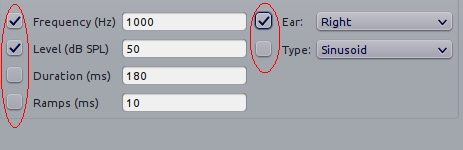
\includegraphics{inSummaryCheckBoxes.png}}
\caption{\code{inSummary} check boxes}\label{engine:fig-insummarycheckboxes}\end{figure}

In the example shown in Figure {\hyperref[engine:fig-insummarycheckboxes]{\emph{inSummary check boxes}}} the frequency,
level and ear parameters will be stored, each in a separate column, in
the block summary table (“\_table”) file, while the parameters
corresponding to the unchecked boxes (duration, ramps and type) will be
not. This is useful if you are running an experiment in which you are
systematically varying only a few parameters across different blocks,
and want to keep track of only those parameters. The \code{inSummary} check
boxes also provide visual landmarks for quickly spotting the widgets
with your parameters of interest in \code{pychoacoustics}.

Notice that the “Process Results Table” function, as mentioned in the
previous section, will average the results for blocks with the same
parameters stored in the block summary table (“\_table”) file. This
means that if you are varying a certain parameter (e.g., level) across
blocks, but you don’t check the corresponding \code{inSummary} check box
(for each block), the value of the parameter will not be stored in the
block summary table (“\_table”) file, and as a consequence the “Process
Results Table” function will not be able to sort the blocks according to
the “level” parameter, and will average the results across all blocks.
Not all is lost, because the “level” parameter will be nonetheless
stored in the “block summary” file, but you will need more work before
you can process your results with a statistical software package.


\subsection{Log Results Files}
\label{engine:log-results-files}
\code{pychoacoustics} automatically saves backup copies of the “block
summary” and “full” files in a backup folder. On Linux systems this
folder is located in

\begin{Verbatim}[commandchars=\\\{\}]
\textasciitilde{}/.local/share/data/pychoacoustics/data\_backup
\end{Verbatim}

on Windows systems it is located in

\begin{Verbatim}[commandchars=\\\{\}]
C:\PYGZbs{}\PYGZbs{}Users\PYGZbs{}username\PYGZbs{}.local\PYGZbs{}share\PYGZbs{}data\PYGZbs{}pychoacoustics\PYGZbs{}data\_backup
\end{Verbatim}

where \code{username} is your account login name. A separate file is saved
for each block of trials that is run. These files are named according to
the date and time at which the blocks were started (the naming follows
the YY-MM-DD-HH-MM-SS scheme). Unlike other results files, that are
written only once a block of trials has been completed, these log
results files get written as soon as information is available (e.g., a
new line in the “full” results file is written at the end of each
trial).


\subsection{Adaptive and Weighted Up/Down Result Files}
\label{engine:adaptive-and-weighted-up-down-result-files}

\subsection{Adaptive and Weighted Up/Down Interleaved Result Files}
\label{engine:adaptive-and-weighted-up-down-interleaved-result-files}

\subsubsection{Constant m-Intervals n-Alternatives Result Files}
\label{engine:constant-m-intervals-n-alternatives-result-files}

\subsubsection{Multiple Constants m-Intervals n-Alternatives Result Files}
\label{engine:multiple-constants-m-intervals-n-alternatives-result-files}

\subsubsection{Constant 1-Intervals 2-Alternatives Result Files}
\label{engine:constant-1-intervals-2-alternatives-result-files}

\subsubsection{Multiple Constants 1-Intervals 2-Alternatives Result Files}
\label{engine:multiple-constants-1-intervals-2-alternatives-result-files}

\subsubsection{Constant 1-Pair Same/Different Result Files}
\label{engine:constant-1-pair-same-different-result-files}

\section{Block Presentation Position}
\label{engine:sec-shuffling}\label{engine:block-presentation-position}
We will define the serial position at which a block is presented during
an experimental session as its “presentation position”, and the serial
position at which a block is stored in a parameters file as its “storage
point”.

Clicking the “Shuffle” button randomises the presentation positions of
the blocks, but leaves the order in which the blocks are stored in a
parameters file untouched. The “Previous” and “Next” buttons, as well as
the “Jump to Block” chooser let you navigate across the blocks storage
points, while the “Previous Position”, and the “Next Position” buttons,
as well as the “Jump to Position” chooser let you navigate across the
blocks presentation positions.

The block presentation positions are recorded in the parameters files.
This is useful in case you have to interrupt an experimental session
whose block presentation positions had been randomized, before it is
finished, and continue it at a later date. In this case you can save the
parameters file, reload it next time, and let the listener complete the
experimental blocks that s/he had not run because of the interruption.
Notice that each time you load a parameters file \code{pychoacoustics} will
automatically move to the first block presentation position. Therefore,
you will have to note down what was the last block that your listener
had run in the interrupted session (or find out by looking at the
results file) and move to the presentation position of the following
block yourself.

By default clicking on the “Shuffle” button performs a simple full
randomization of the block presentation positions. However, you can
specify more complex shuffling schemes in the “Shuffling Scheme” text
field. Let’s say you want to present two tasks in your experiment, a
frequency discrimination and an intensity discrimination task. Each task
has four subconditions, (e.g. four different base frequencies for the
frequency discrimination task and four different base intensities for
the intensity discrimination task). Your parameters file will contain
eight blocks in total, blocks one to four are for the frequency
discrimination task and blocks five to eight are for the intensity
discrimination task. During the experiment you want your participants to
run first the four frequency discrimination conditions in random order,
and afterwards the four intensity discrimination conditions in random
order. To achieve this you can enter the following shuffling scheme:

\begin{Verbatim}[commandchars=\\\{\}]
\PYG{p}{(}\PYG{p}{[}\PYG{l+m+mi}{1}\PYG{p}{,}\PYG{l+m+mi}{2}\PYG{p}{,}\PYG{l+m+mi}{3}\PYG{p}{,}\PYG{l+m+mi}{4}\PYG{p}{]}\PYG{p}{,} \PYG{p}{[}\PYG{l+m+mi}{5}\PYG{p}{,}\PYG{l+m+mi}{6}\PYG{p}{,}\PYG{l+m+mi}{7}\PYG{p}{,}\PYG{l+m+mi}{8}\PYG{p}{]}\PYG{p}{)}
\end{Verbatim}

basically you specify sequences (which can be nested) with your
experimental blocks, sequences within round parentheses \code{()} are not
shuffled, while sequences within square brackets \code{{[}{]}} are shuffled.
Following the previous example, if you want to present first the four
blocks of one of the tasks (either frequency or intensity) in random
order, and then the four blocks of the other task in random order, you
would specify your shuffling scheme as follows:

\begin{Verbatim}[commandchars=\\\{\}]
\PYG{p}{[}\PYG{p}{[}\PYG{l+m+mi}{1}\PYG{p}{,}\PYG{l+m+mi}{2}\PYG{p}{,}\PYG{l+m+mi}{3}\PYG{p}{,}\PYG{l+m+mi}{4}\PYG{p}{]}\PYG{p}{,} \PYG{p}{[}\PYG{l+m+mi}{5}\PYG{p}{,}\PYG{l+m+mi}{6}\PYG{p}{,}\PYG{l+m+mi}{7}\PYG{p}{,}\PYG{l+m+mi}{8}\PYG{p}{]}\PYG{p}{]}
\end{Verbatim}

on the other hand, if you want to present first the four blocks of one
of the tasks (either frequency or intensity) in sequential order and
then the four blocks of the other task in sequential order, you would
specify your shuffling scheme as follows:

\begin{Verbatim}[commandchars=\\\{\}]
\PYG{p}{[}\PYG{p}{(}\PYG{l+m+mi}{1}\PYG{p}{,}\PYG{l+m+mi}{2}\PYG{p}{,}\PYG{l+m+mi}{3}\PYG{p}{,}\PYG{l+m+mi}{4}\PYG{p}{)}\PYG{p}{,} \PYG{p}{(}\PYG{l+m+mi}{5}\PYG{p}{,}\PYG{l+m+mi}{6}\PYG{p}{,}\PYG{l+m+mi}{7}\PYG{p}{,}\PYG{l+m+mi}{8}\PYG{p}{)}\PYG{p}{]}
\end{Verbatim}

you can have any variation you like on the theme, and the lists can be
nested ad libitum, so for example you could have:

\begin{Verbatim}[commandchars=\\\{\}]
\PYG{p}{[}\PYG{p}{(}\PYG{l+m+mi}{1}\PYG{p}{,}\PYG{l+m+mi}{2}\PYG{p}{,}\PYG{p}{[}\PYG{l+m+mi}{3}\PYG{p}{,}\PYG{l+m+mi}{4}\PYG{p}{]}\PYG{p}{)}\PYG{p}{,} \PYG{p}{(}\PYG{l+m+mi}{5}\PYG{p}{,}\PYG{l+m+mi}{6}\PYG{p}{,}\PYG{l+m+mi}{7}\PYG{p}{,}\PYG{l+m+mi}{8}\PYG{p}{)}\PYG{p}{]}
\end{Verbatim}

this would instruct \code{pychoacoustics} to present first either the four
frequency conditions or the four intensity conditions. The first two
frequency conditions are presented sequentially, while the last two are
shuffled. To save typing you can give ranges rather than listing all
blocks individually. For example:

\begin{Verbatim}[commandchars=\\\{\}]
\PYG{p}{(}\PYG{p}{[}\PYG{l+m+mi}{1}\PYG{o}{-}\PYG{l+m+mi}{4}\PYG{p}{]}\PYG{p}{,} \PYG{p}{[}\PYG{l+m+mi}{5}\PYG{o}{-}\PYG{l+m+mi}{8}\PYG{p}{]}\PYG{p}{)}
\end{Verbatim}

is equivalent to:

\begin{Verbatim}[commandchars=\\\{\}]
\PYG{p}{(}\PYG{p}{[}\PYG{l+m+mi}{1}\PYG{p}{,}\PYG{l+m+mi}{2}\PYG{p}{,}\PYG{l+m+mi}{3}\PYG{p}{,}\PYG{l+m+mi}{4}\PYG{p}{]}\PYG{p}{,} \PYG{p}{[}\PYG{l+m+mi}{5}\PYG{p}{,}\PYG{l+m+mi}{6}\PYG{p}{,}\PYG{l+m+mi}{7}\PYG{p}{,}\PYG{l+m+mi}{8}\PYG{p}{]}\PYG{p}{)}
\end{Verbatim}


\section{OS Commands}
\label{engine:os-commands}\label{engine:sec-os-commands}
\code{pychoacoustics} can be instructed to run operating system (OS)
commands at the end of an experiment. This may be useful to run custom
scripts that may analyse the result files, backup result files or
perform other operations.

In the control window, you can enter commands that you want to be
executed at the end of a specific experiment in the ``End Command'' box.
This command will be saved in the parameters file of the experiment.

In the ``Preferences Dialog'', under the ``Notifications'' tab you can
instead set a command that will be executed at the end of each
experiment you run, or $n$ blocks before the end of each
experiment you run. These commands should be entered in the ``Execute
custom command'' boxes.

The commands that you can execute are OS commands, therefore they are
different on Linux and Windows platforms. On Linux, for example,
assuming that you store all your experimental results in the directory
``/home/foo/exp/'', you could automatically make a backup of these files
in the directory ``/home/foo/backup/exp/'' by using the command

\begin{Verbatim}[commandchars=\\\{\}]
\PYG{n+nv}{\PYGZdl{} }rsync -r -t -v --progress -s /home/foo/exp/ /home/foo/backup/exp/
\end{Verbatim}

To make things more interesting, you can use some special strings to
pass \code{pychoacoustics} internal variables to your commands. For
example, if you want to copy the results file of the current experiment
to the directory ``/home/foo/res/'', you can use the command

\begin{Verbatim}[commandchars=\\\{\}]
\PYG{n+nv}{\PYGZdl{} }cp \PYG{o}{[}resFile\PYG{o}{]} /home/foo/backup/exp/
\end{Verbatim}

here the special string \code{{[}resFile{]}} will be converted to the name of
the file where \code{pychoacoustics} has saved the data. A full listing of
these special strings is given in Table {\hyperref[engine:tab-pycho-variables]{\emph{pychoacoustics variables}}}
\phantomsection\label{engine:tab-pycho-variables}

\begin{threeparttable}
\capstart\caption{pychoacoustics variables}

\begin{tabulary}{\linewidth}{|L|L|}
\hline

\textbf{String}
 & 
\textbf{Variable}
\\\hline

\code{{[}resDir{]}}
 & 
Results file directory
\\\hline

\code{{[}resFile{]}}
 & 
Block summary results file
\\\hline

\code{{[}resFileFull{]}}
 & 
Full results file
\\\hline

\code{{[}resFileRes{]}}
 & 
Session summary results file
\\\hline

\code{{[}resTable{]}}
 & 
Block summary table results file
\\\hline

\code{{[}listener{]}}
 & 
Listener label
\\\hline

\code{{[}experimenter{]}}
 & 
Experimenter ID
\\\hline
\end{tabulary}

\end{threeparttable}



\section{Preferences Settings}
\label{engine:preferences-settings}
All the settings that can be manipulated in the
“Preferences” dialog, as well as the “Phones” and “Experimenters”
dialogs are stored in a file in the user home directory. On Linux this
file is located in:

\begin{Verbatim}[commandchars=\\\{\}]
\textasciitilde{}/.config/pychoacoustics/preferences.py
\end{Verbatim}

On Windows, assuming the root drive is “C” it is located in:

\begin{Verbatim}[commandchars=\\\{\}]
C:\PYGZbs{}\PYGZbs{}Users\PYGZbs{}username\PYGZbs{}.config/pychoacoustics\PYGZbs{}preferences.py
\end{Verbatim}

where \code{username} is your Windows login username. Although I strive to
avoid this, the way in which the preferences settings are stored may
change in newer versions of pychoacoustics. This means that when
pychoacoustics is upgraded to a newer version it may sometimes not start
or throw out errors. To address these issues, please, try removing the
old preferences file. Of course this means that you’re going to lose all
the settings that you had previously saved. To avoid loosing any
precious information, such as the calibration values of your headphones,
write down all important info before removing the preferences file.


\section{Response Mode}
\label{engine:response-mode}\label{engine:sec-response-mode}
\code{pychoacoustics} was designed to run interactive experiments in which
a listener hears some stimuli and gives a response through a button or
key press. This is the default mode, called “Real Listener” mode.
\code{pychoacoustics} provides two additional response modes, “Automatic”
and “Simulated Listener”. These modes can be set through the control
window.

In “Automatic” response mode, rather than waiting for the listener to
give a response, \code{pychoacoustics} gives itself a response and proceeds
to the next trial. The probability that this automatic response is
correct can also be set through the control window. The “Automatic”
response mode has two main functions. The first is testing and debugging
an experiment. Rather than running the experiment yourself, you can
launch \code{pychoacoustics} in “Automatic” response mode and check that
everything runs smoothly, the program doesn’t crash, and the result
files are saved correctly. The second function of the automatic response
mode is to allow passive presentation of the stimuli. Some neuroimaging
experiments (e.g. electroencephalographic or functional magnetic
resonance recordings) are performed with listeners passively listening
to the stimuli. These experiments usually also require that the program
presenting the stimuli sends triggers to the recording equipment to flag
the start of a trial. Potentially this can also be done in
\code{pychoacoustics} (and we’ve done it in our lab for
electroencephalographic recordings), but at the moment this
functionality is not implemented in a general way in the program.

The “Simulated Listener” mode is simply a hook that allows you to
redirect the control flow of the program to some code that simulates a
listener and provides a response. Notice that \code{pychoacoustics} does
not provide any simulation code in itself, the simulation code has to be
written by you for a specific experiment. If no simulation code is
written in the experiment file, \code{pychoacoustics} will do nothing in
simulated listenr mode. Further details on how to use the “Simulated
Listener” mode are provided in Section {\hyperref[custom_experiments:sec-simulations]{\emph{Simulations}}}.

Both the “Automatic” and the “Simulated Listener” make recursive
function calls. In Python the number of recursive function calls that
you can make is limited. If your experiment passes this limit
\code{pychoacoustics} will crash. The limit can be raised, up to a certain
extent (which is dependent on your operating system, see the
documentation for the setrecursionlimit function in the Python \code{sys}
module) through the “Max Recursion Depth” setting that you can find in
the preferences window, or set through a command line option when
running \code{pychoacoustics} from the command line. Notice that the total
number of recursive calls that your program will make to complete an
experiments will be higher than the number of trials in the experiment,
so you should set the “Max Recursion Depth” to a value higher than the
number of trials you’re planning to perform (how much higher I don’t
know, you should find out by trial and error, a few hundred points
higher is usually sufficient). If you’re planning to run a very high
number of trials in “Automatic” or “Simulated Listener” mode, rather
than raising the max recursion depth, it may be better to split the
experiment in several parts. You can always write a script that
automatically launches \code{pychoacoustics} from the command line
instructing it to load a given parameters file. On UNIX machines you
could write a shell script to do that, but an easier way is perhaphs to
use python itself to write the script. For example, the \code{python}
script could be:

\begin{Verbatim}[commandchars=\\\{\}]
\PYG{c}{\PYGZsh{}! /usr/bin/env python}
\PYG{k}{for} \PYG{n}{i} \PYG{o+ow}{in} \PYG{n+nb}{range}\PYG{p}{(}\PYG{l+m+mi}{5}\PYG{p}{)}\PYG{p}{:}
   \PYG{n}{cmd} \PYG{o}{=} \PYG{l+s}{"}\PYG{l+s}{pychoacoustics --file prms.prm -l L1 -s s1 -q -a }\PYG{l+s+se}{\PYGZbs{}}
\PYG{l+s}{         --recursion-depth 3000}\PYG{l+s}{"}
\end{Verbatim}

here we’re telling \code{pychoacoustics} to load the parameters file
\code{prms.prm}, set the listener identifier to “L1” and the session label
to s1. The \code{-q} option instructs the program to exit at the end of the
experiment. This way the recursion depth count is effectively restarted
each time \code{pychoacoustics} is closed and launched again from the
script. When the \code{-{-}recursion-depth} option is passed as a command
line argument, as in the example above, it overrides the max recursion
depth value set in the preferences window. If the \code{-a} option is
passed, as in the examples above, \code{pychoacoustics} will start
automatically at the beginning of each of the five series . This is
useful for debugging or simulations, so that you can start the script
and leave the program complete unattended (you need to make sure that
the “Shuffling Mode” is not set to “Ask” and that you pass listener and
session labels if you want the program to run completely unattended).


\chapter{Designing Custom Experiments}
\label{custom_experiments:designing-custom-experiments}\label{custom_experiments::doc}
In order to add a new experiment to \code{pychoacoustics}, create a directory in your home folder called \code{pychoacoustics\_experiments}, inside this folder create a subfolder called \code{custom\_experiments}. Each experiment is written in a single file contained in this folder. Let’s imagine we want to create an experiment for a frequency discrimination task. We create a file named \code{freq.py} in the \code{custom\_experiments} folder. In addition to the experiment file we need an additional file that lists all the experiments contained in the \code{custom\_experiments} directory. This file must be named \code{\_\_init\_\_.py}, and in our case it will have the following content:

\begin{Verbatim}[commandchars=\\\{\}]
\PYG{n}{\PYGZus{}\PYGZus{}all\PYGZus{}\PYGZus{}} \PYG{o}{=} \PYG{p}{[}\PYG{l+s}{"}\PYG{l+s}{freq}\PYG{l+s}{"}\PYG{p}{]}
\end{Verbatim}

here the variable \code{\_\_all\_\_} is simply a python list with the
name of the experiment files. So, if one day we decide to write a new
experiment on, let’s say, level discrimination, in a file called
\code{lev.py} we would simply add it to the list in \code{\_\_init\_\_.py}:

\begin{Verbatim}[commandchars=\\\{\}]
\PYG{n}{\PYGZus{}\PYGZus{}all\PYGZus{}\PYGZus{}} \PYG{o}{=} \PYG{p}{[}\PYG{l+s}{"}\PYG{l+s}{freq}\PYG{l+s}{"}\PYG{p}{,}
           \PYG{l+s}{"}\PYG{l+s}{lev}\PYG{l+s}{"}\PYG{p}{]}
\end{Verbatim}

For people familiar with packaging Python modules it should be clear
by now that the custom experiments folder is basically a Python package
containing various modules (the experiment files). If at some point we
want to remove an experiment from \code{pychoacoustics}, for example
because it contains a bug that does not allow the program to start, we
can simply remove it from the list in \code{\_\_init\_\_.py}.  Let’s go back
to the \code{freq.py} file. Here we need to define four functions. For our
example the names of these functions would be:

\begin{Verbatim}[commandchars=\\\{\}]
\PYG{n}{initialize\PYGZus{}freq}\PYG{p}{(}\PYG{p}{)}
\PYG{n}{select\PYGZus{}default\PYGZus{}parameters\PYGZus{}freq}\PYG{p}{(}\PYG{p}{)}
\PYG{n}{get\PYGZus{}fields\PYGZus{}to\PYGZus{}hide\PYGZus{}freq}\PYG{p}{(}\PYG{p}{)}
\PYG{n}{doTrial\PYGZus{}freq}\PYG{p}{(}\PYG{p}{)}
\end{Verbatim}

basically the function names consist of a fixed prefix, followed by
the name of the experiment file. So in the case of the level experiment
example, written in the file \code{lev.py}, the four functions would be
called:

\begin{Verbatim}[commandchars=\\\{\}]
\PYG{n}{initialize\PYGZus{}lev}\PYG{p}{(}\PYG{p}{)}
\PYG{n}{select\PYGZus{}default\PYGZus{}parameters\PYGZus{}lev}\PYG{p}{(}\PYG{p}{)}
\PYG{n}{get\PYGZus{}fields\PYGZus{}to\PYGZus{}hide\PYGZus{}lev}\PYG{p}{(}\PYG{p}{)}
\PYG{n}{doTrial\PYGZus{}lev}\PYG{p}{(}\PYG{p}{)}
\end{Verbatim}

we’ll look at each function in details shortly. Briefly, the
\code{initialize\_} function is used to set some general parameters and
options for our experiment; the \code{select\_default\_parameters\_} function
lists all the widgets (text fields and choosers) of our experiment and
their default values; the \code{get\_field\_to\_hide\_} function is used to
dinamically hide or show certain widgets depending on the status of
other widgets; finally, the \code{doTrial\_} function contains the code that
generates the sounds and plays them during the experiment.


\section{The \texttt{initialize\_} function}
\label{custom_experiments:the-initialize-function}\begin{quote}

The \code{initialize\_} function of our frequency discrimination experiment looks like this:
\end{quote}

\begin{Verbatim}[commandchars=\\\{\},numbers=left,firstnumber=1,stepnumber=1]
 \PYG{k}{def} \PYG{n+nf}{initialize\PYGZus{}freq}\PYG{p}{(}\PYG{n}{prm}\PYG{p}{)}\PYG{p}{:}
   \PYG{n}{exp\PYGZus{}name} \PYG{o}{=} \PYG{l+s}{"}\PYG{l+s}{Frequency Discrimination Demo}\PYG{l+s}{"}
   \PYG{n}{prm}\PYG{p}{[}\PYG{l+s}{"}\PYG{l+s}{experimentsChoices}\PYG{l+s}{"}\PYG{p}{]}\PYG{o}{.}\PYG{n}{append}\PYG{p}{(}\PYG{n}{exp\PYGZus{}name}\PYG{p}{)}
   \PYG{n}{prm}\PYG{p}{[}\PYG{n}{exp\PYGZus{}name}\PYG{p}{]} \PYG{o}{=} \PYG{p}{\PYGZob{}}\PYG{p}{\PYGZcb{}}
   \PYG{n}{prm}\PYG{p}{[}\PYG{n}{exp\PYGZus{}name}\PYG{p}{]}\PYG{p}{[}\PYG{l+s}{"}\PYG{l+s}{paradigmChoices}\PYG{l+s}{"}\PYG{p}{]} \PYG{o}{=} \PYG{p}{[}\PYG{l+s}{"}\PYG{l+s}{Adaptive}\PYG{l+s}{"}\PYG{p}{,}
                                       \PYG{l+s}{"}\PYG{l+s}{Weighted Up/Down}\PYG{l+s}{"}\PYG{p}{,}
                                       \PYG{l+s}{"}\PYG{l+s}{Constant m-Intervals n-Alternatives}\PYG{l+s}{"}\PYG{p}{]}

   \PYG{n}{prm}\PYG{p}{[}\PYG{n}{exp\PYGZus{}name}\PYG{p}{]}\PYG{p}{[}\PYG{l+s}{"}\PYG{l+s}{opts}\PYG{l+s}{"}\PYG{p}{]} \PYG{o}{=} \PYG{p}{[}\PYG{l+s}{"}\PYG{l+s}{hasISIBox}\PYG{l+s}{"}\PYG{p}{,} \PYG{l+s}{"}\PYG{l+s}{hasAlternativesChooser}\PYG{l+s}{"}\PYG{p}{,}
                            \PYG{l+s}{"}\PYG{l+s}{hasFeedback}\PYG{l+s}{"}\PYG{p}{,} \PYG{l+s}{"}\PYG{l+s}{hasIntervalLights}\PYG{l+s}{"}\PYG{p}{]}

   \PYG{n}{prm}\PYG{p}{[}\PYG{n}{exp\PYGZus{}name}\PYG{p}{]}\PYG{p}{[}\PYG{l+s}{"}\PYG{l+s}{execString}\PYG{l+s}{"}\PYG{p}{]} \PYG{o}{=} \PYG{l+s}{"}\PYG{l+s}{freq}\PYG{l+s}{"}
   \PYG{k}{return} \PYG{n}{prm}
\end{Verbatim}

When the function is called, it is passed a dictionary containing
various parameters through the “prm” argument. The function receives
this dictionary of parameters and adds or modifies some of them. On line 2
we give a label to the experiment, this can be anything we
want, except the label of an experiment already existing. On line 3
we add this experiment label to the list of “experimentsChoices”.
On line 4 we create a new sub-dictionary that has as a key the
experiment label. Next we list the paradims that our experiment
supports by creating a “paradigmChoices” key and giving the names of
the supported paradigms as a list. The paradims listed here must be
within the set of paradims  supported by \code{pychoacoustics} (see
Section {\hyperref[psychophysics:sec-paradigms]{\emph{Available Paradigms}}} for a description of the paradigms currently
supported). In the next line we set an \code{opts} key containing a list
of options. The full list of options that can be set here is described
in details in Section {\hyperref[custom_experiments:sec-experiment-opts]{\emph{The Experiment “opts”}}}. In brief, for our
experiment we want to have a widget to set the ISI between presentation
intervals (\code{hasISIBox}), a widget to choose the number of response
alternatives (\code{hasAlternativesChooser}), a widget to set the feedback
on or off for a given block of trials (\code{hasFeedback}), and finally we
want lights to mark the observation intervals (\code{hasIntervalLights}).
The penultimate line of the \code{initialize\_} function sets the
“\code{execString}” of our experiment. This must be the name of our
experiment file, so in our case “\code{freq}”.


\section{The \texttt{select\_default\_parameters\_} function}
\label{custom_experiments:the-select-default-parameters-function}\begin{quote}

The \code{select\_default\_parameters\_} function is the function in which you define all the widgets (text fields and choosers) needed for your experiment. For our frequency discrimination experiment, the function looks as follows:
\end{quote}

\begin{Verbatim}[commandchars=\\\{\},numbers=left,firstnumber=1,stepnumber=1]
 \PYG{k}{def} \PYG{n+nf}{select\PYGZus{}default\PYGZus{}parameters\PYGZus{}freq}\PYG{p}{(}\PYG{n}{parent}\PYG{p}{,} \PYG{n}{paradigm}\PYG{p}{,} \PYG{n}{par}\PYG{p}{)}\PYG{p}{:}

   \PYG{n}{field} \PYG{o}{=} \PYG{p}{[}\PYG{p}{]}
   \PYG{n}{fieldLabel} \PYG{o}{=} \PYG{p}{[}\PYG{p}{]}
   \PYG{n}{chooser} \PYG{o}{=} \PYG{p}{[}\PYG{p}{]}
   \PYG{n}{chooserLabel} \PYG{o}{=} \PYG{p}{[}\PYG{p}{]}
   \PYG{n}{chooserOptions} \PYG{o}{=} \PYG{p}{[}\PYG{p}{]}

   \PYG{n}{fieldLabel}\PYG{o}{.}\PYG{n}{append}\PYG{p}{(}\PYG{l+s}{"}\PYG{l+s}{Frequency (Hz)}\PYG{l+s}{"}\PYG{p}{)}
   \PYG{n}{field}\PYG{o}{.}\PYG{n}{append}\PYG{p}{(}\PYG{l+m+mi}{1000}\PYG{p}{)}

   \PYG{n}{fieldLabel}\PYG{o}{.}\PYG{n}{append}\PYG{p}{(}\PYG{l+s}{"}\PYG{l+s}{Difference (}\PYG{l+s}{\PYGZpc{}}\PYG{l+s}{)}\PYG{l+s}{"}\PYG{p}{)}
   \PYG{n}{field}\PYG{o}{.}\PYG{n}{append}\PYG{p}{(}\PYG{l+m+mi}{20}\PYG{p}{)}

   \PYG{n}{fieldLabel}\PYG{o}{.}\PYG{n}{append}\PYG{p}{(}\PYG{l+s}{"}\PYG{l+s}{Level (dB SPL)}\PYG{l+s}{"}\PYG{p}{)}
   \PYG{n}{field}\PYG{o}{.}\PYG{n}{append}\PYG{p}{(}\PYG{l+m+mi}{50}\PYG{p}{)}

   \PYG{n}{fieldLabel}\PYG{o}{.}\PYG{n}{append}\PYG{p}{(}\PYG{l+s}{"}\PYG{l+s}{Duration (ms)}\PYG{l+s}{"}\PYG{p}{)}
   \PYG{n}{field}\PYG{o}{.}\PYG{n}{append}\PYG{p}{(}\PYG{l+m+mi}{180}\PYG{p}{)}

   \PYG{n}{fieldLabel}\PYG{o}{.}\PYG{n}{append}\PYG{p}{(}\PYG{l+s}{"}\PYG{l+s}{Ramps (ms)}\PYG{l+s}{"}\PYG{p}{)}
   \PYG{n}{field}\PYG{o}{.}\PYG{n}{append}\PYG{p}{(}\PYG{l+m+mi}{10}\PYG{p}{)}


   \PYG{n}{chooserOptions}\PYG{o}{.}\PYG{n}{append}\PYG{p}{(}\PYG{p}{[}\PYG{l+s}{"}\PYG{l+s}{Right}\PYG{l+s}{"}\PYG{p}{,}
                          \PYG{l+s}{"}\PYG{l+s}{Left}\PYG{l+s}{"}\PYG{p}{,}
                          \PYG{l+s}{"}\PYG{l+s}{Both}\PYG{l+s}{"}\PYG{p}{]}\PYG{p}{)}
   \PYG{n}{chooserLabel}\PYG{o}{.}\PYG{n}{append}\PYG{p}{(}\PYG{l+s}{"}\PYG{l+s}{Ear:}\PYG{l+s}{"}\PYG{p}{)}
   \PYG{n}{chooser}\PYG{o}{.}\PYG{n}{append}\PYG{p}{(}\PYG{l+s}{"}\PYG{l+s}{Right}\PYG{l+s}{"}\PYG{p}{)}

   \PYG{n}{prm} \PYG{o}{=} \PYG{p}{\PYGZob{}}\PYG{p}{\PYGZcb{}}
   \PYG{k}{if} \PYG{n}{paradigm} \PYG{o}{==} \PYG{n+nb+bp}{None}\PYG{p}{:}
       \PYG{n}{prm}\PYG{p}{[}\PYG{l+s}{'}\PYG{l+s}{paradigm}\PYG{l+s}{'}\PYG{p}{]} \PYG{o}{=} \PYG{l+s}{"}\PYG{l+s}{Adaptive}\PYG{l+s}{"}
   \PYG{k}{else}\PYG{p}{:}
       \PYG{n}{prm}\PYG{p}{[}\PYG{l+s}{'}\PYG{l+s}{paradigm}\PYG{l+s}{'}\PYG{p}{]} \PYG{o}{=} \PYG{n}{paradigm}
   \PYG{n}{prm}\PYG{p}{[}\PYG{l+s}{'}\PYG{l+s}{adType}\PYG{l+s}{'}\PYG{p}{]} \PYG{o}{=}  \PYG{l+s}{"}\PYG{l+s}{Geometric}\PYG{l+s}{"}
   \PYG{n}{prm}\PYG{p}{[}\PYG{l+s}{'}\PYG{l+s}{field}\PYG{l+s}{'}\PYG{p}{]} \PYG{o}{=} \PYG{n}{field}
   \PYG{n}{prm}\PYG{p}{[}\PYG{l+s}{'}\PYG{l+s}{fieldLabel}\PYG{l+s}{'}\PYG{p}{]} \PYG{o}{=} \PYG{n}{fieldLabel}
   \PYG{n}{prm}\PYG{p}{[}\PYG{l+s}{'}\PYG{l+s}{chooser}\PYG{l+s}{'}\PYG{p}{]} \PYG{o}{=} \PYG{n}{chooser}
   \PYG{n}{prm}\PYG{p}{[}\PYG{l+s}{'}\PYG{l+s}{chooserLabel}\PYG{l+s}{'}\PYG{p}{]} \PYG{o}{=} \PYG{n}{chooserLabel}
   \PYG{n}{prm}\PYG{p}{[}\PYG{l+s}{'}\PYG{l+s}{chooserOptions}\PYG{l+s}{'}\PYG{p}{]} \PYG{o}{=}  \PYG{n}{chooserOptions}
   \PYG{n}{prm}\PYG{p}{[}\PYG{l+s}{'}\PYG{l+s}{nIntervals}\PYG{l+s}{'}\PYG{p}{]} \PYG{o}{=} \PYG{l+m+mi}{2}
   \PYG{n}{prm}\PYG{p}{[}\PYG{l+s}{'}\PYG{l+s}{nAlternatives}\PYG{l+s}{'}\PYG{p}{]} \PYG{o}{=} \PYG{l+m+mi}{2}

   \PYG{k}{return} \PYG{n}{prm}
\end{Verbatim}

The \code{select\_default\_parameters\_} function accepts three arguments, “parent” is simply a reference to the pychoacoustics application, “paradigm” is the paradigm with which the function has been called, while “par” is a variable that can hold some special values for initializing the function. The use of the
“par” argument is discussed in Section {\hyperref[custom_experiments:sec-par]{\emph{Using par}}}.  From line three to line seven, we create a series of empty lists. The \code{field} and \code{fieldLabel} lists will hold the default values of our text field widgets, and their labels, respectively. The \code{chooser} and \code{chooserLabel} lists will likewise hold the default values of our chooser widgets, and their labels, while the \code{chooserOptions} list will hold  the possible values that our choosers can take. On lines 9 to 29 we populate these lists for our frequency discrimination experiment. The last lines of our \code{select\_default\_parameters\_} function are
used to set some additional parameters. On line 31 we create a dictionary to hold the parameters. On lines 32–35 we set a default paradigm for our experiment if \code{None} has been passed to our function. On line 36 \code{adType} sets the default type of the adaptive procedure, this could be either \code{Geometric}, or \code{Arithmetic}. From line 37 to line 41 we insert in the dictionary the
\code{field}, \code{fieldLabel}, \code{chooser}, \code{chooserLabel} and \code{chooserOptions} lists that we previously creaetd and populated. Finally, on lines 42-43, we give the default number of response intervals and response alternatives.


\section{The \texttt{get\_fields\_to\_hide\_} function}
\label{custom_experiments:the-get-fields-to-hide-function}\begin{quote}

The purpose of the \code{get\_fields\_to\_hide\_} function is to dinamically show or hide certain widgets depending on the status of other widgets. This function must be defined, but is not essential to a \code{pychoacoustics} experiment, so if you want to read all the essential information first, you can simply define the function as follows:
\end{quote}

\begin{Verbatim}[commandchars=\\\{\}]
\PYG{k}{def} \PYG{n+nf}{get\PYGZus{}fields\PYGZus{}to\PYGZus{}hide\PYGZus{}freq}\PYG{p}{(}\PYG{n}{parent}\PYG{p}{)}\PYG{p}{:}
  \PYG{k}{pass}
\end{Verbatim}

and move on to read about the next function, otherwise, read on.
Let’s suppose that you  want to set up a frequency discrimination
experiment in which the frequency of the  standard stimulus may be
either fixed, or change from trial to trial. You start by writing an
experiment with a single “Frequency” text field for the fixed stimulus
frequency case. You then add two additional fields called “Min.
Frequency” and “Max Frequency” to set the range of frequencies in the
roving frequency case. Finally, you create a chooser to decide whether
an experiment is to be run with a fixed or roving frequency. The code
for creating these widgets is shown below:


\section{The \texttt{doTrial\_} function}
\label{custom_experiments:the-dotrial-function}
\begin{Verbatim}[commandchars=\\\{\},numbers=left,firstnumber=1,stepnumber=1]
\PYG{k}{def} \PYG{n+nf}{doTrial\PYGZus{}freq}\PYG{p}{(}\PYG{n}{parent}\PYG{p}{)}\PYG{p}{:}

   \PYG{n}{currBlock} \PYG{o}{=} \PYG{l+s}{'}\PYG{l+s}{b}\PYG{l+s}{'}\PYG{o}{+} \PYG{n+nb}{str}\PYG{p}{(}\PYG{n}{parent}\PYG{o}{.}\PYG{n}{prm}\PYG{p}{[}\PYG{l+s}{'}\PYG{l+s}{currentBlock}\PYG{l+s}{'}\PYG{p}{]}\PYG{p}{)}
    \PYG{k}{if} \PYG{n}{parent}\PYG{o}{.}\PYG{n}{prm}\PYG{p}{[}\PYG{l+s}{'}\PYG{l+s}{startOfBlock}\PYG{l+s}{'}\PYG{p}{]} \PYG{o}{==} \PYG{n+nb+bp}{True}\PYG{p}{:}
        \PYG{n}{parent}\PYG{o}{.}\PYG{n}{prm}\PYG{p}{[}\PYG{l+s}{'}\PYG{l+s}{additional\PYGZus{}parameters\PYGZus{}to\PYGZus{}write}\PYG{l+s}{'}\PYG{p}{]} \PYG{o}{=} \PYG{p}{\PYGZob{}}\PYG{p}{\PYGZcb{}}
        \PYG{n}{parent}\PYG{o}{.}\PYG{n}{prm}\PYG{p}{[}\PYG{l+s}{'}\PYG{l+s}{adaptiveDifference}\PYG{l+s}{'}\PYG{p}{]} \PYG{o}{=} \PYG{n}{parent}\PYG{o}{.}\PYG{n}{prm}\PYG{p}{[}\PYG{n}{currBlock}\PYG{p}{]}\PYG{p}{[}\PYG{l+s}{'}\PYG{l+s}{field}\PYG{l+s}{'}\PYG{p}{]}\PYG{p}{[}\PYG{n}{parent}\PYG{o}{.}\PYG{n}{prm}\PYG{p}{[}\PYG{l+s}{'}\PYG{l+s}{fieldLabel}\PYG{l+s}{'}\PYG{p}{]}\PYG{o}{.}\PYG{n}{index}\PYG{p}{(}\PYG{l+s}{"}\PYG{l+s}{Difference (}\PYG{l+s}{\PYGZpc{}}\PYG{l+s}{)}\PYG{l+s}{"}\PYG{p}{)}\PYG{p}{]}
        \PYG{n}{parent}\PYG{o}{.}\PYG{n}{prm}\PYG{p}{[}\PYG{l+s}{'}\PYG{l+s}{conditions}\PYG{l+s}{'}\PYG{p}{]} \PYG{o}{=} \PYG{p}{[}\PYG{n+nb}{str}\PYG{p}{(}\PYG{n}{parent}\PYG{o}{.}\PYG{n}{prm}\PYG{p}{[}\PYG{l+s}{'}\PYG{l+s}{adaptiveDifference}\PYG{l+s}{'}\PYG{p}{]}\PYG{p}{)}\PYG{p}{]}

        \PYG{n}{parent}\PYG{o}{.}\PYG{n}{writeResultsHeader}\PYG{p}{(}\PYG{l+s}{'}\PYG{l+s}{log}\PYG{l+s}{'}\PYG{p}{)}
    \PYG{n}{parent}\PYG{o}{.}\PYG{n}{currentCondition} \PYG{o}{=} \PYG{n}{parent}\PYG{o}{.}\PYG{n}{prm}\PYG{p}{[}\PYG{l+s}{'}\PYG{l+s}{conditions}\PYG{l+s}{'}\PYG{p}{]}\PYG{p}{[}\PYG{l+m+mi}{0}\PYG{p}{]}

    \PYG{n}{frequency} \PYG{o}{=} \PYG{n}{parent}\PYG{o}{.}\PYG{n}{prm}\PYG{p}{[}\PYG{n}{currBlock}\PYG{p}{]}\PYG{p}{[}\PYG{l+s}{'}\PYG{l+s}{field}\PYG{l+s}{'}\PYG{p}{]}\PYG{p}{[}\PYG{n}{parent}\PYG{o}{.}\PYG{n}{prm}\PYG{p}{[}\PYG{l+s}{'}\PYG{l+s}{fieldLabel}\PYG{l+s}{'}\PYG{p}{]}\PYG{o}{.}\PYG{n}{index}\PYG{p}{(}\PYG{l+s}{"}\PYG{l+s}{Frequency (Hz)}\PYG{l+s}{"}\PYG{p}{)}\PYG{p}{]}
    \PYG{n}{level} \PYG{o}{=} \PYG{n}{parent}\PYG{o}{.}\PYG{n}{prm}\PYG{p}{[}\PYG{n}{currBlock}\PYG{p}{]}\PYG{p}{[}\PYG{l+s}{'}\PYG{l+s}{field}\PYG{l+s}{'}\PYG{p}{]}\PYG{p}{[}\PYG{n}{parent}\PYG{o}{.}\PYG{n}{prm}\PYG{p}{[}\PYG{l+s}{'}\PYG{l+s}{fieldLabel}\PYG{l+s}{'}\PYG{p}{]}\PYG{o}{.}\PYG{n}{index}\PYG{p}{(}\PYG{l+s}{"}\PYG{l+s}{Level (dB SPL)}\PYG{l+s}{"}\PYG{p}{)}\PYG{p}{]}
    \PYG{n}{duration} \PYG{o}{=} \PYG{n}{parent}\PYG{o}{.}\PYG{n}{prm}\PYG{p}{[}\PYG{n}{currBlock}\PYG{p}{]}\PYG{p}{[}\PYG{l+s}{'}\PYG{l+s}{field}\PYG{l+s}{'}\PYG{p}{]}\PYG{p}{[}\PYG{n}{parent}\PYG{o}{.}\PYG{n}{prm}\PYG{p}{[}\PYG{l+s}{'}\PYG{l+s}{fieldLabel}\PYG{l+s}{'}\PYG{p}{]}\PYG{o}{.}\PYG{n}{index}\PYG{p}{(}\PYG{l+s}{"}\PYG{l+s}{Duration (ms)}\PYG{l+s}{"}\PYG{p}{)}\PYG{p}{]}
    \PYG{n}{ramps} \PYG{o}{=} \PYG{n}{parent}\PYG{o}{.}\PYG{n}{prm}\PYG{p}{[}\PYG{n}{currBlock}\PYG{p}{]}\PYG{p}{[}\PYG{l+s}{'}\PYG{l+s}{field}\PYG{l+s}{'}\PYG{p}{]}\PYG{p}{[}\PYG{n}{parent}\PYG{o}{.}\PYG{n}{prm}\PYG{p}{[}\PYG{l+s}{'}\PYG{l+s}{fieldLabel}\PYG{l+s}{'}\PYG{p}{]}\PYG{o}{.}\PYG{n}{index}\PYG{p}{(}\PYG{l+s}{"}\PYG{l+s}{Ramps (ms)}\PYG{l+s}{"}\PYG{p}{)}\PYG{p}{]}
    \PYG{n}{phase} \PYG{o}{=} \PYG{l+m+mi}{0}
    \PYG{n}{channel} \PYG{o}{=} \PYG{n}{parent}\PYG{o}{.}\PYG{n}{prm}\PYG{p}{[}\PYG{n}{currBlock}\PYG{p}{]}\PYG{p}{[}\PYG{l+s}{'}\PYG{l+s}{chooser}\PYG{l+s}{'}\PYG{p}{]}\PYG{p}{[}\PYG{n}{parent}\PYG{o}{.}\PYG{n}{prm}\PYG{p}{[}\PYG{l+s}{'}\PYG{l+s}{chooserLabel}\PYG{l+s}{'}\PYG{p}{]}\PYG{o}{.}\PYG{n}{index}\PYG{p}{(}\PYG{l+s}{"}\PYG{l+s}{Ear:}\PYG{l+s}{"}\PYG{p}{)}\PYG{p}{]}

    \PYG{n}{correctFrequency} \PYG{o}{=} \PYG{n}{frequency} \PYG{o}{+} \PYG{p}{(}\PYG{n}{frequency}\PYG{o}{*}\PYG{n}{parent}\PYG{o}{.}\PYG{n}{prm}\PYG{p}{[}\PYG{l+s}{'}\PYG{l+s}{adaptiveDifference}\PYG{l+s}{'}\PYG{p}{]}\PYG{p}{)}\PYG{o}{/}\PYG{l+m+mi}{100}
    \PYG{n}{parent}\PYG{o}{.}\PYG{n}{stimulusCorrect} \PYG{o}{=} \PYG{n}{pureTone}\PYG{p}{(}\PYG{n}{correctFrequency}\PYG{p}{,} \PYG{n}{phase}\PYG{p}{,} \PYG{n}{level}\PYG{p}{,} \PYG{n}{duration}\PYG{p}{,} \PYG{n}{ramps}\PYG{p}{,} \PYG{n}{channel}\PYG{p}{,} \PYG{n}{parent}\PYG{o}{.}\PYG{n}{prm}\PYG{p}{[}\PYG{l+s}{'}\PYG{l+s}{sampRate}\PYG{l+s}{'}\PYG{p}{]}\PYG{p}{,} \PYG{n}{parent}\PYG{o}{.}\PYG{n}{prm}\PYG{p}{[}\PYG{l+s}{'}\PYG{l+s}{maxLevel}\PYG{l+s}{'}\PYG{p}{]}\PYG{p}{)}

    \PYG{n}{parent}\PYG{o}{.}\PYG{n}{stimulusIncorrect} \PYG{o}{=} \PYG{p}{[}\PYG{p}{]}
    \PYG{k}{for} \PYG{n}{i} \PYG{o+ow}{in} \PYG{n+nb}{range}\PYG{p}{(}\PYG{p}{(}\PYG{n}{parent}\PYG{o}{.}\PYG{n}{prm}\PYG{p}{[}\PYG{l+s}{'}\PYG{l+s}{nIntervals}\PYG{l+s}{'}\PYG{p}{]}\PYG{o}{-}\PYG{l+m+mi}{1}\PYG{p}{)}\PYG{p}{)}\PYG{p}{:}
        \PYG{n}{thisSnd} \PYG{o}{=} \PYG{n}{pureTone}\PYG{p}{(}\PYG{n}{frequency}\PYG{p}{,} \PYG{n}{phase}\PYG{p}{,} \PYG{n}{level}\PYG{p}{,} \PYG{n}{duration}\PYG{p}{,} \PYG{n}{ramps}\PYG{p}{,} \PYG{n}{channel}\PYG{p}{,} \PYG{n}{parent}\PYG{o}{.}\PYG{n}{prm}\PYG{p}{[}\PYG{l+s}{'}\PYG{l+s}{sampRate}\PYG{l+s}{'}\PYG{p}{]}\PYG{p}{,} \PYG{n}{parent}\PYG{o}{.}\PYG{n}{prm}\PYG{p}{[}\PYG{l+s}{'}\PYG{l+s}{maxLevel}\PYG{l+s}{'}\PYG{p}{]}\PYG{p}{)}
        \PYG{n}{parent}\PYG{o}{.}\PYG{n}{stimulusIncorrect}\PYG{o}{.}\PYG{n}{append}\PYG{p}{(}\PYG{n}{thisSnd}\PYG{p}{)}

    \PYG{n}{parent}\PYG{o}{.}\PYG{n}{playRandomisedIntervals}\PYG{p}{(}\PYG{n}{parent}\PYG{o}{.}\PYG{n}{stimulusCorrect}\PYG{p}{,} \PYG{n}{parent}\PYG{o}{.}\PYG{n}{stimulusIncorrect}\PYG{p}{)}
\end{Verbatim}


\section{The Experiment “opts”}
\label{custom_experiments:the-experiment-opts}\label{custom_experiments:sec-experiment-opts}\begin{itemize}
\item {} 
\code{hasISIBox}

\item {} 
\code{hasAlternativesChooser}

\item {} 
\code{hasFeedback}

\item {} 
\code{hasIntervalLights}

\item {} 
\code{hasPreTrialInterval}

\end{itemize}


\section{Using \texttt{par}}
\label{custom_experiments:using-par}\label{custom_experiments:sec-par}

\subsection{Simulations}
\label{custom_experiments:sec-simulations}\label{custom_experiments:simulations}\begin{quote}

\code{pychoacoustics} is not designed to run simulations in itself, however it provides a hook to redirect the control flow to an auditory model that you need to specify yourself in the experiment file.  You can retrieve the current response mode from the experiment file with:
\end{quote}

\begin{Verbatim}[commandchars=\\\{\},numbers=left,firstnumber=1,stepnumber=1]
 \PYG{n}{parent}\PYG{o}{.}\PYG{n}{prm}\PYG{p}{[}\PYG{l+s}{'}\PYG{l+s}{allBlocks}\PYG{l+s}{'}\PYG{p}{]}\PYG{p}{[}\PYG{l+s}{'}\PYG{l+s}{responseMode}\PYG{l+s}{'}\PYG{p}{]}
\end{Verbatim}

so, in the experiment file, after the creation of the stimuli for the trial you can redirect the control flow of the program depending on the response mode:

\begin{Verbatim}[commandchars=\\\{\},numbers=left,firstnumber=1,stepnumber=1]
 \PYG{k}{if} \PYG{n}{parent}\PYG{o}{.}\PYG{n}{prm}\PYG{p}{[}\PYG{l+s}{'}\PYG{l+s}{allBlocks}\PYG{l+s}{'}\PYG{p}{]}\PYG{p}{[}\PYG{l+s}{'}\PYG{l+s}{responseMode}\PYG{l+s}{'}\PYG{p}{]} \PYG{o}{!=} \PYG{l+s}{"}\PYG{l+s}{Simulated Listener}\PYG{l+s}{"}\PYG{p}{:}
    \PYG{c}{\PYGZsh{}we are not in simulation mode, play the stimuli for the listener}
    \PYG{n}{parent}\PYG{o}{.}\PYG{n}{playSoundSequence}\PYG{p}{(}\PYG{n}{sndSeq}\PYG{p}{,} \PYG{n}{ISIs}\PYG{p}{)}
 \PYG{k}{if} \PYG{n}{parent}\PYG{o}{.}\PYG{n}{prm}\PYG{p}{[}\PYG{l+s}{'}\PYG{l+s}{allBlocks}\PYG{l+s}{'}\PYG{p}{]}\PYG{p}{[}\PYG{l+s}{'}\PYG{l+s}{responseMode}\PYG{l+s}{'}\PYG{p}{]} \PYG{o}{==} \PYG{l+s}{"}\PYG{l+s}{Simulated Listener}\PYG{l+s}{"}\PYG{p}{:}
    \PYG{c}{\PYGZsh{}we are in simulation mode}
    \PYG{c}{\PYGZsh{}pass the stimuli to an auditory model and decision device}
    \PYG{c}{\PYGZsh{}---}
    \PYG{c}{\PYGZsh{}Here you specify your model, pychoacoustics doesn't do it for you!}
    \PYG{c}{\PYGZsh{} at the end your simulated listener arrives to a response that is}
    \PYG{c}{\PYGZsh{} either correct or incorrect}
    \PYG{c}{\PYGZsh{}---}
    \PYG{n}{parent}\PYG{o}{.}\PYG{n}{prm}\PYG{p}{[}\PYG{l+s}{'}\PYG{l+s}{trialRunning}\PYG{l+s}{'}\PYG{p}{]} \PYG{o}{=} \PYG{n+nb+bp}{False}
    \PYG{c}{\PYGZsh{}this is needed for technical reasons (if the 'trialRunning'}
    \PYG{c}{\PYGZsh{}flag were set to 'True' pychoacoustics would not process}
    \PYG{c}{\PYGZsh{}the response.}
    \PYG{c}{\PYGZsh{}}
    \PYG{c}{\PYGZsh{}let's suppose that at the end of the simulation you store the}
    \PYG{c}{\PYGZsh{}response in a variable called 'resp', that can take as values}
    \PYG{c}{\PYGZsh{}either the string 'Correct' or the string 'Incorrect'.}
    \PYG{c}{\PYGZsh{}You can then proceed to let pychoacoustics process the response:}
    \PYG{c}{\PYGZsh{}}
    \PYG{k}{if} \PYG{n}{resp} \PYG{o}{==} \PYG{l+s}{'}\PYG{l+s}{Correct}\PYG{l+s}{'}\PYG{p}{:}
       \PYG{n}{parent}\PYG{o}{.}\PYG{n}{sortResponse}\PYG{p}{(}\PYG{n}{parent}\PYG{o}{.}\PYG{n}{correctButton}\PYG{p}{)}
    \PYG{k}{elif} \PYG{n}{resp} \PYG{o}{==} \PYG{l+s}{'}\PYG{l+s}{Incorrect}\PYG{l+s}{'}\PYG{p}{:}
       \PYG{c}{\PYGZsh{}list all the possible 'incorrect' buttons}
       \PYG{n}{inc\PYGZus{}buttons} \PYG{o}{=} \PYG{n}{numpy}\PYG{o}{.}\PYG{n}{delete}\PYG{p}{(}\PYG{n}{numpy}\PYG{o}{.}\PYG{n}{arange}\PYG{p}{(}
                                  \PYG{n+nb+bp}{self}\PYG{o}{.}\PYG{n}{prm}\PYG{p}{[}\PYG{l+s}{'}\PYG{l+s}{nAlternatives}\PYG{l+s}{'}\PYG{p}{]}\PYG{p}{)}\PYG{o}{+}\PYG{l+m+mi}{1}\PYG{p}{,}
                                  \PYG{n+nb+bp}{self}\PYG{o}{.}\PYG{n}{correctButton}\PYG{o}{-}\PYG{l+m+mi}{1}\PYG{p}{)}\PYG{p}{)}
       \PYG{c}{\PYGZsh{}choose one of the incorrect buttons}
       \PYG{n}{parent}\PYG{o}{.}\PYG{n}{sortResponse}\PYG{p}{(}\PYG{n}{random}\PYG{o}{.}\PYG{n}{choice}\PYG{p}{(}\PYG{n}{inc\PYGZus{}buttons}\PYG{p}{)}\PYG{p}{)}
\end{Verbatim}


\chapter{Troubleshooting}
\label{troubleshooting::doc}\label{troubleshooting:troubleshooting}

\section{The computer crashed in the middle of an experimental session}
\label{troubleshooting:the-computer-crashed-in-the-middle-of-an-experimental-session}
\code{pychoacoustics} saves the results at the end of each block, therefore
only the results from the last uncompleted block will be lost, the
results of completed blocks will not be lost. If you have an experiment
with many different blocks presented in random order it may be difficult
to see which blocks the listener had already completed and set
\code{pychoacoustics} to run only the blocks that were not run. To address
this issue \code{pychoacoustics} keeps a copy of the parameters, including
the block presentation order after shuffling, in a file called
\code{.tmp\_prm.prm} (this is a hidden file on Linux systems). Therefore,
after the crash you can simply load this parameters file and move to the
block position that the listener was running when the computer crashed
to resume the experiment.

A second function of the \code{.tmp\_prm.prm} file is to keep a copy of
parameters that were stored in memory, but not saved to a file. If your
computer crashed while you were setting up a parameters for an
experiment that were not yet saved (or were only partially saved) to a
file, you can retrieve them after the crash by loading the
\code{.tmp\_prm.prm} file. One important thing to keep in mind is that the
\code{.tmp\_prm.prm} will be overwritten as soon as new parameters are
stored in memory by a \code{pychoacoustics} instance opened in the same
directory. Therefore it is advisable to make a copy of the
\code{.tmp\_prm.prm} file renaming it to avoid accidentally loosing its
contents after the crash.


\chapter{\texttt{sndlib} -- Sound Synthesis Library}
\label{sndlib:module-sndlib}\label{sndlib::doc}\label{sndlib:sndlib-sound-synthesis-library}\index{sndlib (module)}
A module for generating sounds in python.
\index{AMTone() (in module sndlib)}

\begin{fulllineitems}
\phantomsection\label{sndlib:sndlib.AMTone}\pysiglinewithargsret{\code{sndlib.}\bfcode{AMTone}}{\emph{frequency}, \emph{AMFreq}, \emph{AMDepth}, \emph{phase}, \emph{level}, \emph{duration}, \emph{ramp}, \emph{channel}, \emph{fs}, \emph{maxLevel}}{}
Generate an amplitude modulated tone.
\begin{quote}\begin{description}
\item[{Parameters }] \leavevmode
\textbf{frequency} : float
\begin{quote}

Carrier frequency in hertz.
\end{quote}

\textbf{AMFreq} : float
\begin{quote}

Amplitude modulation frequency in Hz.
\end{quote}

\textbf{AMDepth} : float
\begin{quote}

Amplitude modulation depth (a value of 1
corresponds to 100\% modulation).
\end{quote}

\textbf{phase} : float
\begin{quote}

Starting phase in radians.
\end{quote}

\textbf{level} : float
\begin{quote}

Tone level in dB SPL.
\end{quote}

\textbf{duration} : float
\begin{quote}

Tone duration (excluding ramps) in milliseconds.
\end{quote}

\textbf{ramp} : float
\begin{quote}

Duration of the onset and offset ramps in milliseconds.
The total duration of the sound will be duration+ramp*2.
\end{quote}

\textbf{channel} : string (`Right', `Left' or `Both')
\begin{quote}

Channel in which the tone will be generated.
\end{quote}

\textbf{fs} : int
\begin{quote}

Samplig frequency in Hz.
\end{quote}

\textbf{maxLevel} : float
\begin{quote}

Level in dB SPL output by the soundcard for a sinusoid of amplitude 1.
\end{quote}

\item[{Returns }] \leavevmode
\textbf{snd} : 2-dimensional array of floats

\end{description}\end{quote}
\paragraph{Examples}

\begin{Verbatim}[commandchars=\\\{\}]
\PYG{g+gp}{\PYGZgt{}\PYGZgt{}\PYGZgt{} }\PYG{n}{snd} \PYG{o}{=} \PYG{n}{AMTone}\PYG{p}{(}\PYG{n}{frequency}\PYG{o}{=}\PYG{l+m+mi}{1000}\PYG{p}{,} \PYG{n}{AMFreq}\PYG{o}{=}\PYG{l+m+mi}{20}\PYG{p}{,} \PYG{n}{AMDepth}\PYG{o}{=}\PYG{l+m+mi}{1}\PYG{p}{,} \PYG{n}{phase}\PYG{o}{=}\PYG{l+m+mi}{0}\PYG{p}{,} \PYG{n}{level}\PYG{o}{=}\PYG{l+m+mi}{65}\PYG{p}{,} \PYG{n}{duration}\PYG{o}{=}\PYG{l+m+mi}{180}\PYG{p}{,}
\PYG{g+gp}{... }    \PYG{n}{ramp}\PYG{o}{=}\PYG{l+m+mi}{10}\PYG{p}{,} \PYG{n}{channel}\PYG{o}{=}\PYG{l+s}{'}\PYG{l+s}{Both}\PYG{l+s}{'}\PYG{p}{,} \PYG{n}{fs}\PYG{o}{=}\PYG{l+m+mi}{48000}\PYG{p}{,} \PYG{n}{maxLevel}\PYG{o}{=}\PYG{l+m+mi}{100}\PYG{p}{)}
\end{Verbatim}

\end{fulllineitems}

\index{ERBDistance() (in module sndlib)}

\begin{fulllineitems}
\phantomsection\label{sndlib:sndlib.ERBDistance}\pysiglinewithargsret{\code{sndlib.}\bfcode{ERBDistance}}{\emph{f1}, \emph{f2}}{}
\end{fulllineitems}

\index{FMTone() (in module sndlib)}

\begin{fulllineitems}
\phantomsection\label{sndlib:sndlib.FMTone}\pysiglinewithargsret{\code{sndlib.}\bfcode{FMTone}}{\emph{fc}, \emph{fm}, \emph{mi}, \emph{phase}, \emph{level}, \emph{duration}, \emph{ramp}, \emph{channel}, \emph{fs}, \emph{maxLevel}}{}
Generate a frequency modulated tone.
\begin{quote}\begin{description}
\item[{Parameters }] \leavevmode
\textbf{fc} : float
\begin{quote}

Carrier frequency in hertz. This is the frequency of the tone at fm zero crossing.
\end{quote}

\textbf{fm} : float
\begin{quote}

Modulation frequency in Hz.
\end{quote}

\textbf{mi} : float
\begin{quote}

Modulation index, also called beta and is equal to deltaF/fm, where
deltaF is the maximum deviation of the instantaneous frequency from
the carrier frequency.
\end{quote}

\textbf{phase} : float
\begin{quote}

Starting phase in radians.
\end{quote}

\textbf{level} : float
\begin{quote}

Tone level in dB SPL.
\end{quote}

\textbf{duration} : float
\begin{quote}

Tone duration (excluding ramps) in milliseconds.
\end{quote}

\textbf{ramp} : float
\begin{quote}

Duration of the onset and offset ramps in milliseconds.
The total duration of the sound will be duration+ramp*2.
\end{quote}

\textbf{channel} : `Right', `Left' or `Both'
\begin{quote}

Channel in which the tone will be generated.
\end{quote}

\textbf{fs} : int
\begin{quote}

Samplig frequency in Hz.
\end{quote}

\textbf{maxLevel} : float
\begin{quote}

Level in dB SPL output by the soundcard for a sinusoid of
amplitude 1.
\end{quote}

\item[{Returns }] \leavevmode
\textbf{snd} : 2-dimensional array of floats

\end{description}\end{quote}
\paragraph{Examples}

\begin{Verbatim}[commandchars=\\\{\}]
\PYG{g+gp}{\PYGZgt{}\PYGZgt{}\PYGZgt{} }\PYG{n}{snd} \PYG{o}{=} \PYG{n}{FMTone}\PYG{p}{(}\PYG{n}{fc}\PYG{o}{=}\PYG{l+m+mi}{1000}\PYG{p}{,} \PYG{n}{fm}\PYG{o}{=}\PYG{l+m+mi}{40}\PYG{p}{,} \PYG{n}{mi}\PYG{o}{=}\PYG{l+m+mi}{1}\PYG{p}{,} \PYG{n}{phase}\PYG{o}{=}\PYG{l+m+mi}{0}\PYG{p}{,} \PYG{n}{level}\PYG{o}{=}\PYG{l+m+mi}{55}\PYG{p}{,} \PYG{n}{duration}\PYG{o}{=}\PYG{l+m+mi}{180}\PYG{p}{,}
\PYG{g+gp}{... }    \PYG{n}{ramp}\PYG{o}{=}\PYG{l+m+mi}{10}\PYG{p}{,} \PYG{n}{channel}\PYG{o}{=}\PYG{l+s}{'}\PYG{l+s}{Both}\PYG{l+s}{'}\PYG{p}{,} \PYG{n}{fs}\PYG{o}{=}\PYG{l+m+mi}{48000}\PYG{p}{,} \PYG{n}{maxLevel}\PYG{o}{=}\PYG{l+m+mi}{100}\PYG{p}{)}
\end{Verbatim}

\end{fulllineitems}

\index{addSounds() (in module sndlib)}

\begin{fulllineitems}
\phantomsection\label{sndlib:sndlib.addSounds}\pysiglinewithargsret{\code{sndlib.}\bfcode{addSounds}}{\emph{snd1}, \emph{snd2}, \emph{delay}, \emph{fs}}{}
Add or concatenate two sounds.
\begin{quote}\begin{description}
\item[{Parameters }] \leavevmode
\textbf{snd1} : array of floats
\begin{quote}

First sound.
\end{quote}

\textbf{snd2} : array of floats
\begin{quote}

Second sound.
\end{quote}

\textbf{delay} : float
\begin{quote}

Delay in milliseconds between the onset of `snd1' and the onset of `snd2'
\end{quote}

\textbf{fs} : float
\begin{quote}

Sampling frequency in hertz of the two sounds.
\end{quote}

\item[{Returns }] \leavevmode
\textbf{snd} : 2-dimensional array of floats

\end{description}\end{quote}
\paragraph{Examples}

\begin{Verbatim}[commandchars=\\\{\}]
\PYG{g+gp}{\PYGZgt{}\PYGZgt{}\PYGZgt{} }\PYG{n}{snd1} \PYG{o}{=} \PYG{n}{pureTone}\PYG{p}{(}\PYG{n}{frequency}\PYG{o}{=}\PYG{l+m+mi}{440}\PYG{p}{,} \PYG{n}{phase}\PYG{o}{=}\PYG{l+m+mi}{0}\PYG{p}{,} \PYG{n}{level}\PYG{o}{=}\PYG{l+m+mi}{65}\PYG{p}{,} \PYG{n}{duration}\PYG{o}{=}\PYG{l+m+mi}{180}\PYG{p}{,}
\PYG{g+gp}{... }    \PYG{n}{ramp}\PYG{o}{=}\PYG{l+m+mi}{10}\PYG{p}{,} \PYG{n}{channel}\PYG{o}{=}\PYG{l+s}{'}\PYG{l+s}{Right}\PYG{l+s}{'}\PYG{p}{,} \PYG{n}{fs}\PYG{o}{=}\PYG{l+m+mi}{48000}\PYG{p}{,} \PYG{n}{maxLevel}\PYG{o}{=}\PYG{l+m+mi}{100}\PYG{p}{)}
\PYG{g+gp}{\PYGZgt{}\PYGZgt{}\PYGZgt{} }\PYG{n}{snd2} \PYG{o}{=} \PYG{n}{pureTone}\PYG{p}{(}\PYG{n}{frequency}\PYG{o}{=}\PYG{l+m+mi}{880}\PYG{p}{,} \PYG{n}{phase}\PYG{o}{=}\PYG{l+m+mi}{0}\PYG{p}{,} \PYG{n}{level}\PYG{o}{=}\PYG{l+m+mi}{65}\PYG{p}{,} \PYG{n}{duration}\PYG{o}{=}\PYG{l+m+mi}{180}\PYG{p}{,}
\PYG{g+gp}{... }    \PYG{n}{ramp}\PYG{o}{=}\PYG{l+m+mi}{10}\PYG{p}{,} \PYG{n}{channel}\PYG{o}{=}\PYG{l+s}{'}\PYG{l+s}{Right}\PYG{l+s}{'}\PYG{p}{,} \PYG{n}{fs}\PYG{o}{=}\PYG{l+m+mi}{48000}\PYG{p}{,} \PYG{n}{maxLevel}\PYG{o}{=}\PYG{l+m+mi}{100}\PYG{p}{)}
\PYG{g+gp}{\PYGZgt{}\PYGZgt{}\PYGZgt{} }\PYG{n}{snd} \PYG{o}{=} \PYG{n}{addSounds}\PYG{p}{(}\PYG{n}{snd1}\PYG{o}{=}\PYG{n}{snd1}\PYG{p}{,} \PYG{n}{snd2}\PYG{o}{=}\PYG{n}{snd2}\PYG{p}{,} \PYG{n}{delay}\PYG{o}{=}\PYG{l+m+mi}{100}\PYG{p}{,} \PYG{n}{fs}\PYG{o}{=}\PYG{l+m+mi}{48000}\PYG{p}{)}
\end{Verbatim}

\end{fulllineitems}

\index{binauralPureTone() (in module sndlib)}

\begin{fulllineitems}
\phantomsection\label{sndlib:sndlib.binauralPureTone}\pysiglinewithargsret{\code{sndlib.}\bfcode{binauralPureTone}}{\emph{frequency}, \emph{phase}, \emph{level}, \emph{duration}, \emph{ramp}, \emph{channel}, \emph{itd}, \emph{itdRef}, \emph{ild}, \emph{ildRef}, \emph{fs}, \emph{maxLevel}}{}
Generate a pure tone with an optional interaural time or level difference.
\begin{quote}\begin{description}
\item[{Parameters }] \leavevmode
\textbf{frequency} : float
\begin{quote}

Tone frequency in hertz.
\end{quote}

\textbf{phase} : float
\begin{quote}

Starting phase in radians.
\end{quote}

\textbf{level} : float
\begin{quote}

Tone level in dB SPL. If `ild' is different than zero, this will
be the level of the tone in the reference channel.
\end{quote}

\textbf{duration} : float
\begin{quote}

Tone duration (excluding ramps) in milliseconds.
\end{quote}

\textbf{ramp} : float
\begin{quote}

Duration of the onset and offset ramps in milliseconds.
The total duration of the sound will be duration+ramp*2.
\end{quote}

\textbf{channel} : string (`Right', `Left' or `Both')
\begin{quote}

Channel in which the tone will be generated.
\end{quote}

\textbf{itd} : float
\begin{quote}

Interaural time difference, in microseconds.
\end{quote}

\textbf{itdRef} : `Right', `Left' or None
\begin{quote}

The reference channel for the `itd'. The interaural time
difference will be applied to the other channel with
respect to the reference channel.
\end{quote}

\textbf{ild} : float
\begin{quote}

Interaural level difference in dB SPL.
\end{quote}

\textbf{ildRef} : `Right', `Left' or None
\begin{quote}

The reference channel for the `ild'.
The level of the other channel will be
icreased of attenuated by `ild' dB SPL
with respect to the reference channel.
\end{quote}

\textbf{fs} : int
\begin{quote}

Samplig frequency in Hz.
\end{quote}

\textbf{maxLevel} : float
\begin{quote}

Level in dB SPL output by the soundcard for a sinusoid of amplitude 1.
\end{quote}

\item[{Returns }] \leavevmode
\textbf{snd} : 2-dimensional array of floats
\begin{quote}

The array has dimensions (nSamples, 2).
\end{quote}

\end{description}\end{quote}
\paragraph{Examples}

\begin{Verbatim}[commandchars=\\\{\}]
\PYG{g+gp}{\PYGZgt{}\PYGZgt{}\PYGZgt{} }\PYG{n}{itdTone} \PYG{o}{=} \PYG{n}{binauralPureTone}\PYG{p}{(}\PYG{n}{frequency}\PYG{o}{=}\PYG{l+m+mi}{440}\PYG{p}{,} \PYG{n}{phase}\PYG{o}{=}\PYG{l+m+mi}{0}\PYG{p}{,} \PYG{n}{level}\PYG{o}{=}\PYG{l+m+mi}{65}\PYG{p}{,} \PYG{n}{duration}\PYG{o}{=}\PYG{l+m+mi}{180}\PYG{p}{,}
\PYG{g+gp}{... }    \PYG{n}{ramp}\PYG{o}{=}\PYG{l+m+mi}{10}\PYG{p}{,} \PYG{n}{channel}\PYG{o}{=}\PYG{l+s}{'}\PYG{l+s}{Both}\PYG{l+s}{'}\PYG{p}{,} \PYG{n}{itd}\PYG{o}{=}\PYG{l+m+mi}{480}\PYG{p}{,} \PYG{n}{itdRef}\PYG{o}{=}\PYG{l+s}{'}\PYG{l+s}{Right}\PYG{l+s}{'}\PYG{p}{,} \PYG{n}{ild}\PYG{o}{=}\PYG{l+m+mi}{0}\PYG{p}{,} \PYG{n}{ildRef}\PYG{o}{=}\PYG{n+nb+bp}{None}\PYG{p}{,}
\PYG{g+gp}{... }    \PYG{n}{fs}\PYG{o}{=}\PYG{l+m+mi}{48000}\PYG{p}{,} \PYG{n}{maxLevel}\PYG{o}{=}\PYG{l+m+mi}{100}\PYG{p}{)}
\PYG{g+gp}{\PYGZgt{}\PYGZgt{}\PYGZgt{} }\PYG{n}{ildTone} \PYG{o}{=} \PYG{n}{binauralPureTone}\PYG{p}{(}\PYG{n}{frequency}\PYG{o}{=}\PYG{l+m+mi}{440}\PYG{p}{,} \PYG{n}{phase}\PYG{o}{=}\PYG{l+m+mi}{0}\PYG{p}{,} \PYG{n}{level}\PYG{o}{=}\PYG{l+m+mi}{65}\PYG{p}{,} \PYG{n}{duration}\PYG{o}{=}\PYG{l+m+mi}{180}\PYG{p}{,}
\PYG{g+gp}{... }    \PYG{n}{ramp}\PYG{o}{=}\PYG{l+m+mi}{10}\PYG{p}{,} \PYG{n}{channel}\PYG{o}{=}\PYG{l+s}{'}\PYG{l+s}{Both}\PYG{l+s}{'}\PYG{p}{,} \PYG{n}{itd}\PYG{o}{=}\PYG{l+m+mi}{0}\PYG{p}{,} \PYG{n}{itdRef}\PYG{o}{=}\PYG{n+nb+bp}{None}\PYG{p}{,} \PYG{n}{ild}\PYG{o}{=}\PYG{o}{-}\PYG{l+m+mi}{20}\PYG{p}{,} \PYG{n}{ildRef}\PYG{o}{=}\PYG{l+s}{'}\PYG{l+s}{Right}\PYG{l+s}{'}\PYG{p}{,}
\PYG{g+gp}{... }    \PYG{n}{fs}\PYG{o}{=}\PYG{l+m+mi}{48000}\PYG{p}{,} \PYG{n}{maxLevel}\PYG{o}{=}\PYG{l+m+mi}{100}\PYG{p}{)}
\end{Verbatim}

\end{fulllineitems}

\index{broadbandNoise() (in module sndlib)}

\begin{fulllineitems}
\phantomsection\label{sndlib:sndlib.broadbandNoise}\pysiglinewithargsret{\code{sndlib.}\bfcode{broadbandNoise}}{\emph{spectrumLevel}, \emph{duration}, \emph{ramp}, \emph{channel}, \emph{fs}, \emph{maxLevel}}{}
Synthetise a broadband noise.
\begin{quote}\begin{description}
\item[{Parameters }] \leavevmode
\textbf{spectrumLevel} : float
\begin{quote}

Intensity spectrum level of the noise in dB SPL.
\end{quote}

\textbf{duration} : float
\begin{quote}

Noise duration (excluding ramps) in milliseconds.
\end{quote}

\textbf{ramp} : float
\begin{quote}

Duration of the onset and offset ramps in milliseconds.
The total duration of the sound will be duration+ramp*2.
\end{quote}

\textbf{channel} : string (`Right', `Left' or `Both')
\begin{quote}

Channel in which the noise will be generated.
\end{quote}

\textbf{fs} : int
\begin{quote}

Samplig frequency in Hz.
\end{quote}

\textbf{maxLevel} : float
\begin{quote}

Level in dB SPL output by the soundcard for a sinusoid of amplitude 1.
\end{quote}

\item[{Returns }] \leavevmode
\textbf{snd} : 2-dimensional array of floats
\begin{quote}

The array has dimensions (nSamples, 2).
\end{quote}

\end{description}\end{quote}
\paragraph{Examples}

\begin{Verbatim}[commandchars=\\\{\}]
\PYG{g+gp}{\PYGZgt{}\PYGZgt{}\PYGZgt{} }\PYG{n}{noise} \PYG{o}{=} \PYG{n}{broadbandNoise}\PYG{p}{(}\PYG{n}{spectrumLevel}\PYG{o}{=}\PYG{l+m+mi}{40}\PYG{p}{,} \PYG{n}{duration}\PYG{o}{=}\PYG{l+m+mi}{180}\PYG{p}{,} \PYG{n}{ramp}\PYG{o}{=}\PYG{l+m+mi}{10}\PYG{p}{,}
\PYG{g+gp}{... }    \PYG{n}{channel}\PYG{o}{=}\PYG{l+s}{'}\PYG{l+s}{Both}\PYG{l+s}{'}\PYG{p}{,} \PYG{n}{fs}\PYG{o}{=}\PYG{l+m+mi}{48000}\PYG{p}{,} \PYG{n}{maxLevel}\PYG{o}{=}\PYG{l+m+mi}{100}\PYG{p}{)}
\end{Verbatim}

\end{fulllineitems}

\index{camSinFMComplex() (in module sndlib)}

\begin{fulllineitems}
\phantomsection\label{sndlib:sndlib.camSinFMComplex}\pysiglinewithargsret{\code{sndlib.}\bfcode{camSinFMComplex}}{\emph{F0}, \emph{lowHarm}, \emph{highHarm}, \emph{harmPhase}, \emph{fm}, \emph{deltaCams}, \emph{fmPhase}, \emph{level}, \emph{duration}, \emph{ramp}, \emph{channel}, \emph{fs}, \emph{maxLevel}}{}
Generate a tone frequency modulated with an exponential sinusoid.
\begin{quote}\begin{description}
\item[{Parameters }] \leavevmode
\textbf{fc} : float
\begin{quote}

Carrier frequency in hertz.
\end{quote}

\textbf{fm} : float
\begin{quote}

Modulation frequency in Hz.
\end{quote}

\textbf{deltaCams} : float
\begin{quote}

Frequency excursion in cam units (ERBn number scale).
\end{quote}

\textbf{fmPhase} : float
\begin{quote}

Starting fmPhase in radians.
\end{quote}

\textbf{level} : float
\begin{quote}

Tone level in dB SPL.
\end{quote}

\textbf{duration} : float
\begin{quote}

Tone duration (excluding ramps) in milliseconds.
\end{quote}

\textbf{ramp} : float
\begin{quote}

Duration of the onset and offset ramps in milliseconds.
The total duration of the sound will be duration+ramp*2.
\end{quote}

\textbf{channel} : `Right', `Left' or `Both'
\begin{quote}

Channel in which the tone will be generated.
\end{quote}

\textbf{fs} : int
\begin{quote}

Samplig frequency in Hz.
\end{quote}

\textbf{maxLevel} : float
\begin{quote}

Level in dB SPL output by the soundcard for a sinusoid of
amplitude 1.
\end{quote}

\item[{Returns }] \leavevmode
\textbf{snd} : 2-dimensional array of floats

\end{description}\end{quote}
\paragraph{Examples}

\begin{Verbatim}[commandchars=\\\{\}]
\PYG{g+gp}{\PYGZgt{}\PYGZgt{}\PYGZgt{} }\PYG{n}{snd} \PYG{o}{=} \PYG{n}{expSinFMTone}\PYG{p}{(}\PYG{n}{fc}\PYG{o}{=}\PYG{l+m+mi}{1000}\PYG{p}{,} \PYG{n}{fm}\PYG{o}{=}\PYG{l+m+mi}{40}\PYG{p}{,} \PYG{n}{deltaCents}\PYG{o}{=}\PYG{l+m+mi}{1200}\PYG{p}{,} \PYG{n}{fmPhase}\PYG{o}{=}\PYG{l+m+mi}{0}\PYG{p}{,} \PYG{n}{level}\PYG{o}{=}\PYG{l+m+mi}{55}\PYG{p}{,} 
\PYG{g+gp}{... }    \PYG{n}{duration}\PYG{o}{=}\PYG{l+m+mi}{180}\PYG{p}{,} \PYG{n}{ramp}\PYG{o}{=}\PYG{l+m+mi}{10}\PYG{p}{,} \PYG{n}{channel}\PYG{o}{=}\PYG{l+s}{'}\PYG{l+s}{Both}\PYG{l+s}{'}\PYG{p}{,} \PYG{n}{fs}\PYG{o}{=}\PYG{l+m+mi}{48000}\PYG{p}{,} \PYG{n}{maxLevel}\PYG{o}{=}\PYG{l+m+mi}{100}\PYG{p}{)}
\end{Verbatim}

\end{fulllineitems}

\index{camSinFMTone() (in module sndlib)}

\begin{fulllineitems}
\phantomsection\label{sndlib:sndlib.camSinFMTone}\pysiglinewithargsret{\code{sndlib.}\bfcode{camSinFMTone}}{\emph{fc}, \emph{fm}, \emph{deltaCams}, \emph{fmPhase}, \emph{startPhase}, \emph{level}, \emph{duration}, \emph{ramp}, \emph{channel}, \emph{fs}, \emph{maxLevel}}{}
Generate a tone frequency modulated with an exponential sinusoid.
\begin{quote}\begin{description}
\item[{Parameters }] \leavevmode
\textbf{fc} : float
\begin{quote}

Carrier frequency in hertz.
\end{quote}

\textbf{fm} : float
\begin{quote}

Modulation frequency in Hz.
\end{quote}

\textbf{deltaCams} : float
\begin{quote}

Frequency excursion in cam units (ERBn number scale).
\end{quote}

\textbf{fmPhase} : float
\begin{quote}

Starting fmPhase in radians.
\end{quote}

\textbf{level} : float
\begin{quote}

Tone level in dB SPL.
\end{quote}

\textbf{duration} : float
\begin{quote}

Tone duration (excluding ramps) in milliseconds.
\end{quote}

\textbf{ramp} : float
\begin{quote}

Duration of the onset and offset ramps in milliseconds.
The total duration of the sound will be duration+ramp*2.
\end{quote}

\textbf{channel} : `Right', `Left' or `Both'
\begin{quote}

Channel in which the tone will be generated.
\end{quote}

\textbf{fs} : int
\begin{quote}

Samplig frequency in Hz.
\end{quote}

\textbf{maxLevel} : float
\begin{quote}

Level in dB SPL output by the soundcard for a sinusoid of
amplitude 1.
\end{quote}

\item[{Returns }] \leavevmode
\textbf{snd} : 2-dimensional array of floats

\end{description}\end{quote}
\paragraph{Examples}

\begin{Verbatim}[commandchars=\\\{\}]
\PYG{g+gp}{\PYGZgt{}\PYGZgt{}\PYGZgt{} }\PYG{n}{snd} \PYG{o}{=} \PYG{n}{expSinFMTone}\PYG{p}{(}\PYG{n}{fc}\PYG{o}{=}\PYG{l+m+mi}{1000}\PYG{p}{,} \PYG{n}{fm}\PYG{o}{=}\PYG{l+m+mi}{40}\PYG{p}{,} \PYG{n}{deltaCents}\PYG{o}{=}\PYG{l+m+mi}{1200}\PYG{p}{,} \PYG{n}{fmPhase}\PYG{o}{=}\PYG{l+m+mi}{0}\PYG{p}{,} \PYG{n}{level}\PYG{o}{=}\PYG{l+m+mi}{55}\PYG{p}{,} 
\PYG{g+gp}{... }    \PYG{n}{duration}\PYG{o}{=}\PYG{l+m+mi}{180}\PYG{p}{,} \PYG{n}{ramp}\PYG{o}{=}\PYG{l+m+mi}{10}\PYG{p}{,} \PYG{n}{channel}\PYG{o}{=}\PYG{l+s}{'}\PYG{l+s}{Both}\PYG{l+s}{'}\PYG{p}{,} \PYG{n}{fs}\PYG{o}{=}\PYG{l+m+mi}{48000}\PYG{p}{,} \PYG{n}{maxLevel}\PYG{o}{=}\PYG{l+m+mi}{100}\PYG{p}{)}
\end{Verbatim}

\end{fulllineitems}

\index{chirp() (in module sndlib)}

\begin{fulllineitems}
\phantomsection\label{sndlib:sndlib.chirp}\pysiglinewithargsret{\code{sndlib.}\bfcode{chirp}}{\emph{freqStart}, \emph{ftype}, \emph{rate}, \emph{level}, \emph{duration}, \emph{phase}, \emph{ramp}, \emph{channel}, \emph{fs}, \emph{maxLevel}}{}
Synthetize a chirp, that is a tone with frequency changing linearly or
exponentially over time with a give rate.
\begin{quote}\begin{description}
\item[{Parameters }] \leavevmode
\textbf{freqStart} : float
\begin{quote}

Starting frequency in hertz.
\end{quote}

\textbf{ftype} : string
\begin{quote}

If `linear', the frequency will change linearly on a Hz scale.
If `exponential', the frequency will change exponentially on a cents scale.
\end{quote}

\textbf{rate} : float
\begin{quote}

Rate of frequency change, Hz/s if ftype is `linear',
and cents/s if ftype is `exponential'.
\end{quote}

\textbf{level} : float
\begin{quote}

Level of the tone in dB SPL.
\end{quote}

\textbf{duration} : float
\begin{quote}

Tone duration (excluding ramps) in milliseconds.
\end{quote}

\textbf{ramp} : float
\begin{quote}

Duration of the onset and offset ramps in milliseconds.
The total duration of the sound will be duration+ramp*2.
\end{quote}

\textbf{channel} : string (`Right', `Left' or `Both')
\begin{quote}

Channel in which the tone will be generated.
\end{quote}

\textbf{fs} : int
\begin{quote}

Samplig frequency in Hz.
\end{quote}

\textbf{maxLevel} : float
\begin{quote}

Level in dB SPL output by the soundcard for a sinusoid of amplitude 1.
\end{quote}

\item[{Returns }] \leavevmode
\textbf{snd} : 2-dimensional array of floats
\begin{quote}

The array has dimensions (nSamples, 2).
\end{quote}

\end{description}\end{quote}
\paragraph{Examples}

\begin{Verbatim}[commandchars=\\\{\}]
\PYG{g+gp}{\PYGZgt{}\PYGZgt{}\PYGZgt{} }\PYG{n}{gl} \PYG{o}{=} \PYG{n}{chirp}\PYG{p}{(}\PYG{n}{freqStart}\PYG{o}{=}\PYG{l+m+mi}{440}\PYG{p}{,} \PYG{n}{ftype}\PYG{o}{=}\PYG{l+s}{'}\PYG{l+s}{linear}\PYG{l+s}{'}\PYG{p}{,} \PYG{n}{rate}\PYG{o}{=}\PYG{l+m+mi}{500}\PYG{p}{,} \PYG{n}{level}\PYG{o}{=}\PYG{l+m+mi}{55}\PYG{p}{,}
\PYG{g+go}{        duration=980, phase=0, ramp=10, channel='Both',}
\PYG{g+go}{        fs=48000, maxLevel=100)}
\end{Verbatim}

\end{fulllineitems}

\index{complexTone() (in module sndlib)}

\begin{fulllineitems}
\phantomsection\label{sndlib:sndlib.complexTone}\pysiglinewithargsret{\code{sndlib.}\bfcode{complexTone}}{\emph{F0}, \emph{harmPhase}, \emph{lowHarm}, \emph{highHarm}, \emph{stretch}, \emph{level}, \emph{duration}, \emph{ramp}, \emph{channel}, \emph{fs}, \emph{maxLevel}}{}
Synthetise a complex tone.
\begin{quote}\begin{description}
\item[{Parameters }] \leavevmode
\textbf{F0} : float
\begin{quote}

Tone fundamental frequency in hertz.
\end{quote}

\textbf{harmPhase} : one of `Sine', `Cosine', `Alternating', `Random', `Schroeder'
\begin{quote}

Phase relationship between the partials of the complex tone.
\end{quote}

\textbf{lowHarm} : int
\begin{quote}

Lowest harmonic component number.
\end{quote}

\textbf{highHarm} : int
\begin{quote}

Highest harmonic component number.
\end{quote}

\textbf{stretch} : float
\begin{quote}

Harmonic stretch in \%F0. Increase each harmonic frequency by a fixed value
that is equal to (F0*stretch)/100. If `stretch' is different than
zero, an inhanmonic complex tone will be generated.
\end{quote}

\textbf{level} : float
\begin{quote}

The level of each partial in dB SPL.
\end{quote}

\textbf{duration} : float
\begin{quote}

Tone duration (excluding ramps) in milliseconds.
\end{quote}

\textbf{ramp} : float
\begin{quote}

Duration of the onset and offset ramps in milliseconds.
The total duration of the sound will be duration+ramp*2.
\end{quote}

\textbf{channel} : `Right', `Left', `Both', `Odd Right' or `Odd Left'
\begin{quote}

Channel in which the tone will be generated. If `channel'
if `Odd Right', odd numbered harmonics will be presented
to the right channel and even number harmonics to the left
channel. The opposite is true if `channel' is `Odd Left'.
\end{quote}

\textbf{fs} : int
\begin{quote}

Samplig frequency in Hz.
\end{quote}

\textbf{maxLevel} : float
\begin{quote}

Level in dB SPL output by the soundcard for a sinusoid of amplitude 1.
\end{quote}

\item[{Returns }] \leavevmode
\textbf{snd} : 2-dimensional array of floats
\begin{quote}

The array has dimensions (nSamples, 2).
\end{quote}

\end{description}\end{quote}
\paragraph{Examples}

\begin{Verbatim}[commandchars=\\\{\}]
\PYG{g+gp}{\PYGZgt{}\PYGZgt{}\PYGZgt{} }\PYG{n}{ct} \PYG{o}{=} \PYG{n}{complexTone}\PYG{p}{(}\PYG{n}{F0}\PYG{o}{=}\PYG{l+m+mi}{440}\PYG{p}{,} \PYG{n}{harmPhase}\PYG{o}{=}\PYG{l+s}{'}\PYG{l+s}{Sine}\PYG{l+s}{'}\PYG{p}{,} \PYG{n}{lowHarm}\PYG{o}{=}\PYG{l+m+mi}{3}\PYG{p}{,} \PYG{n}{highHarm}\PYG{o}{=}\PYG{l+m+mi}{10}\PYG{p}{,}
\PYG{g+gp}{... }    \PYG{n}{stretch}\PYG{o}{=}\PYG{l+m+mi}{0}\PYG{p}{,} \PYG{n}{level}\PYG{o}{=}\PYG{l+m+mi}{55}\PYG{p}{,} \PYG{n}{duration}\PYG{o}{=}\PYG{l+m+mi}{180}\PYG{p}{,} \PYG{n}{ramp}\PYG{o}{=}\PYG{l+m+mi}{10}\PYG{p}{,} \PYG{n}{channel}\PYG{o}{=}\PYG{l+s}{'}\PYG{l+s}{Both}\PYG{l+s}{'}\PYG{p}{,}
\PYG{g+gp}{... }    \PYG{n}{fs}\PYG{o}{=}\PYG{l+m+mi}{48000}\PYG{p}{,} \PYG{n}{maxLevel}\PYG{o}{=}\PYG{l+m+mi}{100}\PYG{p}{)}
\end{Verbatim}

\end{fulllineitems}

\index{complexToneParallel() (in module sndlib)}

\begin{fulllineitems}
\phantomsection\label{sndlib:sndlib.complexToneParallel}\pysiglinewithargsret{\code{sndlib.}\bfcode{complexToneParallel}}{\emph{F0}, \emph{harmPhase}, \emph{lowHarm}, \emph{highHarm}, \emph{stretch}, \emph{level}, \emph{duration}, \emph{ramp}, \emph{channel}, \emph{fs}, \emph{maxLevel}}{}
Synthetise a complex tone.

This function produces the same results of complexTone. The only difference
is that it uses the multiprocessing Python module to exploit multicore
processors and compute the partials in a parallel fashion. Notice that
there is a substantial overhead in setting up the parallel computations.
This means that for relatively short sounds (in the order of seconds),
this function will actually be \emph{slower} than complexTone.
\begin{quote}\begin{description}
\item[{Parameters }] \leavevmode
\textbf{F0} : float
\begin{quote}

Tone fundamental frequency in hertz.
\end{quote}

\textbf{harmPhase} : one of `Sine', `Cosine', `Alternating', `Random', `Schroeder'
\begin{quote}

Phase relationship between the partials of the complex tone.
\end{quote}

\textbf{lowHarm} : int
\begin{quote}

Lowest harmonic component number.
\end{quote}

\textbf{highHarm} : int
\begin{quote}

Highest harmonic component number.
\end{quote}

\textbf{stretch} : float
\begin{quote}

Harmonic stretch in \%F0. Increase each harmonic frequency by a fixed value
that is equal to (F0*stretch)/100. If `stretch' is different than
zero, an inhanmonic complex tone will be generated.
\end{quote}

\textbf{level} : float
\begin{quote}

The level of each partial in dB SPL.
\end{quote}

\textbf{duration} : float
\begin{quote}

Tone duration (excluding ramps) in milliseconds.
\end{quote}

\textbf{ramp} : float
\begin{quote}

Duration of the onset and offset ramps in milliseconds.
The total duration of the sound will be duration+ramp*2.
\end{quote}

\textbf{channel} : `Right', `Left', `Both', `Odd Right' or `Odd Left'
\begin{quote}

Channel in which the tone will be generated. If `channel'
if `Odd Right', odd numbered harmonics will be presented
to the right channel and even number harmonics to the left
channel. The opposite is true if `channel' is `Odd Left'.
\end{quote}

\textbf{fs} : int
\begin{quote}

Samplig frequency in Hz.
\end{quote}

\textbf{maxLevel} : float
\begin{quote}

Level in dB SPL output by the soundcard for a sinusoid of amplitude 1.
\end{quote}

\item[{Returns }] \leavevmode
\textbf{snd} : 2-dimensional array of floats
\begin{quote}

The array has dimensions (nSamples, 2).
\end{quote}

\end{description}\end{quote}
\paragraph{Examples}

\begin{Verbatim}[commandchars=\\\{\}]
\PYG{g+gp}{\PYGZgt{}\PYGZgt{}\PYGZgt{} }\PYG{n}{ct} \PYG{o}{=} \PYG{n}{complexTone}\PYG{p}{(}\PYG{n}{F0}\PYG{o}{=}\PYG{l+m+mi}{440}\PYG{p}{,} \PYG{n}{harmPhase}\PYG{o}{=}\PYG{l+s}{'}\PYG{l+s}{Sine}\PYG{l+s}{'}\PYG{p}{,} \PYG{n}{lowHarm}\PYG{o}{=}\PYG{l+m+mi}{3}\PYG{p}{,} \PYG{n}{highHarm}\PYG{o}{=}\PYG{l+m+mi}{10}\PYG{p}{,}
\PYG{g+gp}{... }    \PYG{n}{stretch}\PYG{o}{=}\PYG{l+m+mi}{0}\PYG{p}{,} \PYG{n}{level}\PYG{o}{=}\PYG{l+m+mi}{55}\PYG{p}{,} \PYG{n}{duration}\PYG{o}{=}\PYG{l+m+mi}{180}\PYG{p}{,} \PYG{n}{ramp}\PYG{o}{=}\PYG{l+m+mi}{10}\PYG{p}{,} \PYG{n}{channel}\PYG{o}{=}\PYG{l+s}{'}\PYG{l+s}{Both}\PYG{l+s}{'}\PYG{p}{,}
\PYG{g+gp}{... }    \PYG{n}{fs}\PYG{o}{=}\PYG{l+m+mi}{48000}\PYG{p}{,} \PYG{n}{maxLevel}\PYG{o}{=}\PYG{l+m+mi}{100}\PYG{p}{)}
\end{Verbatim}

\end{fulllineitems}

\index{expAMNoise() (in module sndlib)}

\begin{fulllineitems}
\phantomsection\label{sndlib:sndlib.expAMNoise}\pysiglinewithargsret{\code{sndlib.}\bfcode{expAMNoise}}{\emph{fc}, \emph{fm}, \emph{deltaCents}, \emph{fmPhase}, \emph{AMDepth}, \emph{spectrumLevel}, \emph{duration}, \emph{ramp}, \emph{channel}, \emph{fs}, \emph{maxLevel}}{}
Generate a sinusoidally amplitude-modulated noise with an exponentially
modulated AM frequency.
\begin{quote}\begin{description}
\item[{Parameters }] \leavevmode
\textbf{fc} : float
\begin{quote}

Carrier AM frequency in hertz.
\end{quote}

\textbf{fm} : float
\begin{quote}

Modulation of the AM frequency in Hz.
\end{quote}

\textbf{deltaCents} : float
\begin{quote}
\begin{description}
\item[{AM frequency excursion in cents. The instataneous AM frequency of the noise}] \leavevmode
will vary from fc**(-deltaCents/1200) to fc**(+deltaCents/1200).

\end{description}
\end{quote}

\textbf{fmPhase} : float
\begin{quote}

Starting phase of the AM modulation in radians.
\end{quote}

\textbf{AMDepth} : float
\begin{quote}

Amplitude modulation depth.
\end{quote}

\textbf{spectrumLevel} : float
\begin{quote}

Noise spectrum level in dB SPL.
\end{quote}

\textbf{duration} : float
\begin{quote}

Tone duration (excluding ramps) in milliseconds.
\end{quote}

\textbf{ramp} : float
\begin{quote}

Duration of the onset and offset ramps in milliseconds.
The total duration of the sound will be duration+ramp*2.
\end{quote}

\textbf{channel} : `Right', `Left' or `Both'
\begin{quote}

Channel in which the tone will be generated.
\end{quote}

\textbf{fs} : int
\begin{quote}

Samplig frequency in Hz.
\end{quote}

\textbf{maxLevel} : float
\begin{quote}

Level in dB SPL output by the soundcard for a sinusoid of
amplitude 1.
\end{quote}

\item[{Returns }] \leavevmode
\textbf{snd} : 2-dimensional array of floats

\end{description}\end{quote}
\paragraph{Examples}

\begin{Verbatim}[commandchars=\\\{\}]
\PYG{g+gp}{\PYGZgt{}\PYGZgt{}\PYGZgt{} }\PYG{n}{snd} \PYG{o}{=} \PYG{n}{expAMNoise}\PYG{p}{(}\PYG{n}{fc}\PYG{o}{=}\PYG{l+m+mi}{150}\PYG{p}{,} \PYG{n}{fm}\PYG{o}{=}\PYG{l+m+mf}{2.4}\PYG{p}{,} \PYG{n}{deltaCents}\PYG{o}{=}\PYG{l+m+mi}{1200}\PYG{p}{,} \PYG{n}{fmPhase}\PYG{o}{=}\PYG{l+m+mf}{3.14}\PYG{p}{,} \PYG{n}{AMDepth} \PYG{o}{=} \PYG{l+m+mi}{1}\PYG{p}{,}
\PYG{g+gp}{... }    \PYG{n}{spectrumLevel}\PYG{o}{=}\PYG{l+m+mi}{24}\PYG{p}{,} \PYG{n}{duration}\PYG{o}{=}\PYG{l+m+mi}{380}\PYG{p}{,} \PYG{n}{ramp}\PYG{o}{=}\PYG{l+m+mi}{10}\PYG{p}{,} \PYG{n}{channel}\PYG{o}{=}\PYG{l+s}{'}\PYG{l+s}{Both}\PYG{l+s}{'}\PYG{p}{,} \PYG{n}{fs}\PYG{o}{=}\PYG{l+m+mi}{48000}\PYG{p}{,} \PYG{n}{maxLevel}\PYG{o}{=}\PYG{l+m+mi}{100}\PYG{p}{)}
\end{Verbatim}

\end{fulllineitems}

\index{expSinFMComplex() (in module sndlib)}

\begin{fulllineitems}
\phantomsection\label{sndlib:sndlib.expSinFMComplex}\pysiglinewithargsret{\code{sndlib.}\bfcode{expSinFMComplex}}{\emph{F0}, \emph{lowHarm}, \emph{highHarm}, \emph{harmPhase}, \emph{fm}, \emph{deltaCents}, \emph{fmPhase}, \emph{level}, \emph{duration}, \emph{ramp}, \emph{channel}, \emph{fs}, \emph{maxLevel}}{}
Generate a frequency-modulated complex tone with an exponential sinusoid.
\begin{quote}\begin{description}
\item[{Parameters }] \leavevmode
\textbf{fc} : float
\begin{quote}

Carrier frequency in hertz.
\end{quote}

\textbf{fm} : float
\begin{quote}

Modulation frequency in Hz.
\end{quote}

\textbf{deltaCents} : float
\begin{quote}
\begin{description}
\item[{Frequency excursion in cents. The instataneous frequency of the tone}] \leavevmode
will vary from fc**(-deltaCents/1200) to fc**(+deltaCents/1200).

\end{description}
\end{quote}

\textbf{fmPhase} : float
\begin{quote}

Starting fmPhase in radians.
\end{quote}

\textbf{level} : float
\begin{quote}

Tone level in dB SPL.
\end{quote}

\textbf{duration} : float
\begin{quote}

Tone duration (excluding ramps) in milliseconds.
\end{quote}

\textbf{ramp} : float
\begin{quote}

Duration of the onset and offset ramps in milliseconds.
The total duration of the sound will be duration+ramp*2.
\end{quote}

\textbf{channel} : `Right', `Left' or `Both'
\begin{quote}

Channel in which the tone will be generated.
\end{quote}

\textbf{fs} : int
\begin{quote}

Samplig frequency in Hz.
\end{quote}

\textbf{maxLevel} : float
\begin{quote}

Level in dB SPL output by the soundcard for a sinusoid of
amplitude 1.
\end{quote}

\item[{Returns }] \leavevmode
\textbf{snd} : 2-dimensional array of floats

\end{description}\end{quote}
\paragraph{Examples}

\begin{Verbatim}[commandchars=\\\{\}]
\PYG{g+gp}{\PYGZgt{}\PYGZgt{}\PYGZgt{} }\PYG{n}{snd} \PYG{o}{=} \PYG{n}{expSinFMTone}\PYG{p}{(}\PYG{n}{fc}\PYG{o}{=}\PYG{l+m+mi}{1000}\PYG{p}{,} \PYG{n}{fm}\PYG{o}{=}\PYG{l+m+mi}{40}\PYG{p}{,} \PYG{n}{deltaCents}\PYG{o}{=}\PYG{l+m+mi}{1200}\PYG{p}{,} \PYG{n}{fmPhase}\PYG{o}{=}\PYG{l+m+mi}{0}\PYG{p}{,} \PYG{n}{level}\PYG{o}{=}\PYG{l+m+mi}{55}\PYG{p}{,} 
\PYG{g+gp}{... }    \PYG{n}{duration}\PYG{o}{=}\PYG{l+m+mi}{180}\PYG{p}{,} \PYG{n}{ramp}\PYG{o}{=}\PYG{l+m+mi}{10}\PYG{p}{,} \PYG{n}{channel}\PYG{o}{=}\PYG{l+s}{'}\PYG{l+s}{Both}\PYG{l+s}{'}\PYG{p}{,} \PYG{n}{fs}\PYG{o}{=}\PYG{l+m+mi}{48000}\PYG{p}{,} \PYG{n}{maxLevel}\PYG{o}{=}\PYG{l+m+mi}{100}\PYG{p}{)}
\end{Verbatim}

\end{fulllineitems}

\index{expSinFMTone() (in module sndlib)}

\begin{fulllineitems}
\phantomsection\label{sndlib:sndlib.expSinFMTone}\pysiglinewithargsret{\code{sndlib.}\bfcode{expSinFMTone}}{\emph{fc}, \emph{fm}, \emph{deltaCents}, \emph{fmPhase}, \emph{startPhase}, \emph{level}, \emph{duration}, \emph{ramp}, \emph{channel}, \emph{fs}, \emph{maxLevel}}{}
Generate a frequency-modulated tone with an exponential sinusoid.
\begin{quote}\begin{description}
\item[{Parameters }] \leavevmode
\textbf{fc} : float
\begin{quote}

Carrier frequency in hertz.
\end{quote}

\textbf{fm} : float
\begin{quote}

Modulation frequency in Hz.
\end{quote}

\textbf{deltaCents} : float
\begin{quote}
\begin{description}
\item[{Frequency excursion in cents. The instataneous frequency of the tone}] \leavevmode
will vary from fc**(-deltaCents/1200) to fc**(+deltaCents/1200).

\end{description}
\end{quote}

\textbf{fmPhase} : float
\begin{quote}

Starting fmPhase in radians.
\end{quote}

\textbf{level} : float
\begin{quote}

Tone level in dB SPL.
\end{quote}

\textbf{duration} : float
\begin{quote}

Tone duration (excluding ramps) in milliseconds.
\end{quote}

\textbf{ramp} : float
\begin{quote}

Duration of the onset and offset ramps in milliseconds.
The total duration of the sound will be duration+ramp*2.
\end{quote}

\textbf{channel} : `Right', `Left' or `Both'
\begin{quote}

Channel in which the tone will be generated.
\end{quote}

\textbf{fs} : int
\begin{quote}

Samplig frequency in Hz.
\end{quote}

\textbf{maxLevel} : float
\begin{quote}

Level in dB SPL output by the soundcard for a sinusoid of
amplitude 1.
\end{quote}

\item[{Returns }] \leavevmode
\textbf{snd} : 2-dimensional array of floats

\end{description}\end{quote}
\paragraph{Examples}

\begin{Verbatim}[commandchars=\\\{\}]
\PYG{g+gp}{\PYGZgt{}\PYGZgt{}\PYGZgt{} }\PYG{n}{snd} \PYG{o}{=} \PYG{n}{expSinFMTone}\PYG{p}{(}\PYG{n}{fc}\PYG{o}{=}\PYG{l+m+mi}{1000}\PYG{p}{,} \PYG{n}{fm}\PYG{o}{=}\PYG{l+m+mi}{40}\PYG{p}{,} \PYG{n}{deltaCents}\PYG{o}{=}\PYG{l+m+mi}{1200}\PYG{p}{,} \PYG{n}{fmPhase}\PYG{o}{=}\PYG{l+m+mi}{0}\PYG{p}{,} \PYG{n}{level}\PYG{o}{=}\PYG{l+m+mi}{55}\PYG{p}{,} 
\PYG{g+gp}{... }    \PYG{n}{duration}\PYG{o}{=}\PYG{l+m+mi}{180}\PYG{p}{,} \PYG{n}{ramp}\PYG{o}{=}\PYG{l+m+mi}{10}\PYG{p}{,} \PYG{n}{channel}\PYG{o}{=}\PYG{l+s}{'}\PYG{l+s}{Both}\PYG{l+s}{'}\PYG{p}{,} \PYG{n}{fs}\PYG{o}{=}\PYG{l+m+mi}{48000}\PYG{p}{,} \PYG{n}{maxLevel}\PYG{o}{=}\PYG{l+m+mi}{100}\PYG{p}{)}
\end{Verbatim}

\end{fulllineitems}

\index{fir2Filt() (in module sndlib)}

\begin{fulllineitems}
\phantomsection\label{sndlib:sndlib.fir2Filt}\pysiglinewithargsret{\code{sndlib.}\bfcode{fir2Filt}}{\emph{f1}, \emph{f2}, \emph{f3}, \emph{f4}, \emph{snd}, \emph{fs}}{}
Filter signal with a fir2 filter.

This function designs and applies a fir2 filter to a sound.
The frequency response of the ideal filter will transition
from 0 to 1 between `f1' and `f2', and from 1 to zero
between `f3' and `f4'. The frequencies must be given in
increasing order.
\begin{quote}\begin{description}
\item[{Parameters }] \leavevmode
\textbf{f1} : float
\begin{quote}

Frequency in hertz of the point at which the transition
for the low-frequency cutoff ends.
\end{quote}

\textbf{f2} : float
\begin{quote}

Frequency in hertz of the point at which the transition
for the low-frequency cutoff starts.
\end{quote}

\textbf{f3} : float
\begin{quote}

Frequency in hertz of the point at which the transition
for the high-frequency cutoff starts.
\end{quote}

\textbf{f4} : float
\begin{quote}

Frequency in hertz of the point at which the transition
for the high-frequency cutoff ends.
\end{quote}

\textbf{snd} : array of floats
\begin{quote}

The sound to be filtered.
\end{quote}

\textbf{fs} : int
\begin{quote}

Sampling frequency of `snd'.
\end{quote}

\item[{Returns }] \leavevmode
\textbf{snd} : 2-dimensional array of floats

\end{description}\end{quote}
\paragraph{Notes}

If `f1' and `f2' are zero the filter will be lowpass.
If `f3' and `f4' are equal to or greater than the nyquist
frequency (fs/2) the filter will be highpass.
In the other cases the filter will be bandpass.

The order of the filter (number of taps) is fixed at 256.
This function uses internally `scipy.signal.firwin2'.
\paragraph{Examples}

\begin{Verbatim}[commandchars=\\\{\}]
\PYG{g+gp}{\PYGZgt{}\PYGZgt{}\PYGZgt{} }\PYG{n}{noise} \PYG{o}{=} \PYG{n}{broadbandNoise}\PYG{p}{(}\PYG{n}{spectrumLevel}\PYG{o}{=}\PYG{l+m+mi}{40}\PYG{p}{,} \PYG{n}{duration}\PYG{o}{=}\PYG{l+m+mi}{180}\PYG{p}{,} \PYG{n}{ramp}\PYG{o}{=}\PYG{l+m+mi}{10}\PYG{p}{,}
\PYG{g+gp}{... }    \PYG{n}{channel}\PYG{o}{=}\PYG{l+s}{'}\PYG{l+s}{Both}\PYG{l+s}{'}\PYG{p}{,} \PYG{n}{fs}\PYG{o}{=}\PYG{l+m+mi}{48000}\PYG{p}{,} \PYG{n}{maxLevel}\PYG{o}{=}\PYG{l+m+mi}{100}\PYG{p}{)}
\PYG{g+gp}{\PYGZgt{}\PYGZgt{}\PYGZgt{} }\PYG{n}{lpNoise} \PYG{o}{=} \PYG{n}{fir2Filt}\PYG{p}{(}\PYG{n}{f1}\PYG{o}{=}\PYG{l+m+mi}{0}\PYG{p}{,} \PYG{n}{f2}\PYG{o}{=}\PYG{l+m+mi}{0}\PYG{p}{,} \PYG{n}{f3}\PYG{o}{=}\PYG{l+m+mi}{1000}\PYG{p}{,} \PYG{n}{f4}\PYG{o}{=}\PYG{l+m+mi}{1200}\PYG{p}{,} 
\PYG{g+gp}{... }    \PYG{n}{snd}\PYG{o}{=}\PYG{n}{noise}\PYG{p}{,} \PYG{n}{fs}\PYG{o}{=}\PYG{l+m+mi}{48000}\PYG{p}{)} \PYG{c}{\PYGZsh{}lowpass filter}
\PYG{g+gp}{\PYGZgt{}\PYGZgt{}\PYGZgt{} }\PYG{n}{hpNoise} \PYG{o}{=} \PYG{n}{fir2Filt}\PYG{p}{(}\PYG{n}{f1}\PYG{o}{=}\PYG{l+m+mi}{0}\PYG{p}{,} \PYG{n}{f2}\PYG{o}{=}\PYG{l+m+mi}{0}\PYG{p}{,} \PYG{n}{f3}\PYG{o}{=}\PYG{l+m+mi}{24000}\PYG{p}{,} \PYG{n}{f4}\PYG{o}{=}\PYG{l+m+mi}{26000}\PYG{p}{,} 
\PYG{g+gp}{... }    \PYG{n}{snd}\PYG{o}{=}\PYG{n}{noise}\PYG{p}{,} \PYG{n}{fs}\PYG{o}{=}\PYG{l+m+mi}{48000}\PYG{p}{)} \PYG{c}{\PYGZsh{}highpass filter}
\PYG{g+gp}{\PYGZgt{}\PYGZgt{}\PYGZgt{} }\PYG{n}{bpNoise} \PYG{o}{=} \PYG{n}{fir2Filt}\PYG{p}{(}\PYG{n}{f1}\PYG{o}{=}\PYG{l+m+mi}{400}\PYG{p}{,} \PYG{n}{f2}\PYG{o}{=}\PYG{l+m+mi}{600}\PYG{p}{,} \PYG{n}{f3}\PYG{o}{=}\PYG{l+m+mi}{4000}\PYG{p}{,} \PYG{n}{f4}\PYG{o}{=}\PYG{l+m+mi}{4400}\PYG{p}{,} 
\PYG{g+gp}{... }    \PYG{n}{snd}\PYG{o}{=}\PYG{n}{noise}\PYG{p}{,} \PYG{n}{fs}\PYG{o}{=}\PYG{l+m+mi}{48000}\PYG{p}{)} \PYG{c}{\PYGZsh{}bandpass filter}
\end{Verbatim}

\end{fulllineitems}

\index{freqFromERBInterval() (in module sndlib)}

\begin{fulllineitems}
\phantomsection\label{sndlib:sndlib.freqFromERBInterval}\pysiglinewithargsret{\code{sndlib.}\bfcode{freqFromERBInterval}}{\emph{f1}, \emph{deltaERB}}{}
\end{fulllineitems}

\index{gate() (in module sndlib)}

\begin{fulllineitems}
\phantomsection\label{sndlib:sndlib.gate}\pysiglinewithargsret{\code{sndlib.}\bfcode{gate}}{\emph{ramps}, \emph{sig}, \emph{fs}}{}
Impose onset and offset ramps to a sound.
\begin{quote}\begin{description}
\item[{Parameters }] \leavevmode
\textbf{ramps} : float
\begin{quote}

The duration of the ramps.
\end{quote}

\textbf{sig} : array of floats
\begin{quote}

The signal on which the ramps should be imposed.
\end{quote}

\textbf{fs} : int
\begin{quote}

The sampling frequency os `sig'
\end{quote}

\item[{Returns }] \leavevmode
\textbf{sig} : array of floats
\begin{quote}

The ramped signal.
\end{quote}

\end{description}\end{quote}
\paragraph{Examples}

\begin{Verbatim}[commandchars=\\\{\}]
\PYG{g+gp}{\PYGZgt{}\PYGZgt{}\PYGZgt{} }\PYG{n}{noise} \PYG{o}{=} \PYG{n}{broadbandNoise}\PYG{p}{(}\PYG{n}{spectrumLevel}\PYG{o}{=}\PYG{l+m+mi}{40}\PYG{p}{,} \PYG{n}{duration}\PYG{o}{=}\PYG{l+m+mi}{200}\PYG{p}{,} \PYG{n}{ramp}\PYG{o}{=}\PYG{l+m+mi}{0}\PYG{p}{,}
\PYG{g+gp}{... }    \PYG{n}{channel}\PYG{o}{=}\PYG{l+s}{'}\PYG{l+s}{Both}\PYG{l+s}{'}\PYG{p}{,} \PYG{n}{fs}\PYG{o}{=}\PYG{l+m+mi}{48000}\PYG{p}{,} \PYG{n}{maxLevel}\PYG{o}{=}\PYG{l+m+mi}{100}\PYG{p}{)}
\PYG{g+gp}{\PYGZgt{}\PYGZgt{}\PYGZgt{} }\PYG{n}{gate}\PYG{p}{(}\PYG{n}{ramps}\PYG{o}{=}\PYG{l+m+mi}{10}\PYG{p}{,} \PYG{n}{sig}\PYG{o}{=}\PYG{n}{noise}\PYG{p}{,} \PYG{n}{fs}\PYG{o}{=}\PYG{l+m+mi}{48000}\PYG{p}{)}
\end{Verbatim}

\end{fulllineitems}

\index{getRms() (in module sndlib)}

\begin{fulllineitems}
\phantomsection\label{sndlib:sndlib.getRms}\pysiglinewithargsret{\code{sndlib.}\bfcode{getRms}}{\emph{sig}}{}
Compute the root mean square (RMS) value of the signal.
\begin{quote}\begin{description}
\item[{Parameters }] \leavevmode
\textbf{sig} : array of floats
\begin{quote}

The signal for which the RMS needs to be computed.
\end{quote}

\item[{Returns }] \leavevmode
\textbf{rms} : float
\begin{quote}

The RMS of `sig'.
\end{quote}

\end{description}\end{quote}
\paragraph{Examples}

\begin{Verbatim}[commandchars=\\\{\}]
\PYG{g+gp}{\PYGZgt{}\PYGZgt{}\PYGZgt{} }\PYG{n}{pt} \PYG{o}{=} \PYG{n}{pureTone}\PYG{p}{(}\PYG{n}{frequency}\PYG{o}{=}\PYG{l+m+mi}{440}\PYG{p}{,} \PYG{n}{phase}\PYG{o}{=}\PYG{l+m+mi}{0}\PYG{p}{,} \PYG{n}{level}\PYG{o}{=}\PYG{l+m+mi}{65}\PYG{p}{,} \PYG{n}{duration}\PYG{o}{=}\PYG{l+m+mi}{180}\PYG{p}{,}
\PYG{g+gp}{... }    \PYG{n}{ramp}\PYG{o}{=}\PYG{l+m+mi}{10}\PYG{p}{,} \PYG{n}{channel}\PYG{o}{=}\PYG{l+s}{'}\PYG{l+s}{Right}\PYG{l+s}{'}\PYG{p}{,} \PYG{n}{fs}\PYG{o}{=}\PYG{l+m+mi}{48000}\PYG{p}{,} \PYG{n}{maxLevel}\PYG{o}{=}\PYG{l+m+mi}{100}\PYG{p}{)}
\PYG{g+gp}{\PYGZgt{}\PYGZgt{}\PYGZgt{} }\PYG{n}{getRms}\PYG{p}{(}\PYG{n}{pt}\PYG{p}{)}
\end{Verbatim}

\end{fulllineitems}

\index{glide() (in module sndlib)}

\begin{fulllineitems}
\phantomsection\label{sndlib:sndlib.glide}\pysiglinewithargsret{\code{sndlib.}\bfcode{glide}}{\emph{freqStart}, \emph{ftype}, \emph{excursion}, \emph{level}, \emph{duration}, \emph{phase}, \emph{ramp}, \emph{channel}, \emph{fs}, \emph{maxLevel}}{}
Synthetize a rising or falling tone glide with frequency changing
linearly or exponentially.
\begin{quote}\begin{description}
\item[{Parameters }] \leavevmode
\textbf{freqStart} : float
\begin{quote}

Starting frequency in hertz.
\end{quote}

\textbf{ftype} : string
\begin{quote}

If `linear', the frequency will change linearly on a Hz scale.
If `exponential', the frequency will change exponentially on a cents scale.
\end{quote}

\textbf{excursion} : float
\begin{quote}

If ftype is `linear', excursion is the total frequency change in Hz.
The final frequency will be freqStart + excursion.
If ftype is `exponential', excursion is the total frequency change in cents.
The final frequency in Hz will be freqStart*2**(excusrion/1200).
\end{quote}

\textbf{level} : float
\begin{quote}

Level of the tone in dB SPL.
\end{quote}

\textbf{duration} : float
\begin{quote}

Tone duration (excluding ramps) in milliseconds.
\end{quote}

\textbf{ramp} : float
\begin{quote}

Duration of the onset and offset ramps in milliseconds.
The total duration of the sound will be duration+ramp*2.
\end{quote}

\textbf{channel} : string (`Right', `Left' or `Both')
\begin{quote}

Channel in which the tone will be generated.
\end{quote}

\textbf{fs} : int
\begin{quote}

Samplig frequency in Hz.
\end{quote}

\textbf{maxLevel} : float
\begin{quote}

Level in dB SPL output by the soundcard for a sinusoid of amplitude 1.
\end{quote}

\item[{Returns }] \leavevmode
\textbf{snd} : 2-dimensional array of floats
\begin{quote}

The array has dimensions (nSamples, 2).
\end{quote}

\end{description}\end{quote}
\paragraph{Examples}

\begin{Verbatim}[commandchars=\\\{\}]
\PYG{g+gp}{\PYGZgt{}\PYGZgt{}\PYGZgt{} }\PYG{n}{gl} \PYG{o}{=} \PYG{n}{glide}\PYG{p}{(}\PYG{n}{freqStart}\PYG{o}{=}\PYG{l+m+mi}{440}\PYG{p}{,} \PYG{n+nb}{type}\PYG{o}{=}\PYG{l+s}{'}\PYG{l+s}{exponential}\PYG{l+s}{'}\PYG{p}{,} \PYG{n}{excursion}\PYG{o}{=}\PYG{l+m+mi}{500}\PYG{p}{,}
\PYG{g+go}{        level=55, duration=180, phase=0, ramp=10, channel='Both',}
\PYG{g+go}{        fs=48000, maxLevel=100)}
\end{Verbatim}

\end{fulllineitems}

\index{harmComplFromNarrowbandNoise() (in module sndlib)}

\begin{fulllineitems}
\phantomsection\label{sndlib:sndlib.harmComplFromNarrowbandNoise}\pysiglinewithargsret{\code{sndlib.}\bfcode{harmComplFromNarrowbandNoise}}{\emph{F0}, \emph{lowHarm}, \emph{highHarm}, \emph{level}, \emph{bandwidth}, \emph{duration}, \emph{ramp}, \emph{channel}, \emph{fs}, \emph{maxLevel}}{}
Generate an harmonic complex tone from narrow noise bands.
\begin{quote}\begin{description}
\item[{Parameters }] \leavevmode
\textbf{F0} : float
\begin{quote}

Fundamental frequency of the complex.
\end{quote}

\textbf{lowHarm} : int
\begin{quote}

Lowest harmonic component number. The first component is \#1.
\end{quote}

\textbf{highHarm} : int
\begin{quote}

Highest harmonic component number.
\end{quote}

\textbf{level} : float
\begin{quote}

The spectrum level of the noise bands in dB SPL.
\end{quote}

\textbf{bandwidth} : float
\begin{quote}

The width of each noise band in hertz.
\end{quote}

\textbf{duration} : float
\begin{quote}

Tone duration (excluding ramps) in milliseconds.
\end{quote}

\textbf{ramp} : float
\begin{quote}

Duration of the onset and offset ramps in milliseconds.
The total duration of the sound will be duration+ramp*2.
\end{quote}

\textbf{channel} : `Right', `Left', `Both', `Odd Right' or `Odd Left'
\begin{quote}

Channel in which the tone will be generated. If `channel'
if `Odd Right', odd numbered harmonics will be presented
to the right channel and even number harmonics to the left
channel. The opposite is true if `channel' is `Odd Left'.
\end{quote}

\textbf{fs} : int
\begin{quote}

Samplig frequency in Hz.
\end{quote}

\textbf{maxLevel} : float
\begin{quote}

Level in dB SPL output by the soundcard for a sinusoid of amplitude 1.
\end{quote}

\item[{Returns }] \leavevmode
\textbf{snd} : array of floats

\end{description}\end{quote}
\paragraph{Examples}

\begin{Verbatim}[commandchars=\\\{\}]
\PYG{g+gp}{\PYGZgt{}\PYGZgt{}\PYGZgt{} }\PYG{n}{c1} \PYG{o}{=} \PYG{n}{harmComplFromNarrowbandNoise}\PYG{p}{(}\PYG{n}{F0}\PYG{o}{=}\PYG{l+m+mi}{440}\PYG{p}{,} \PYG{n}{lowHarm}\PYG{o}{=}\PYG{l+m+mi}{3}\PYG{p}{,} \PYG{n}{highHarm}\PYG{o}{=}\PYG{l+m+mi}{8}\PYG{p}{,}
\PYG{g+go}{     level=40, bandwidth=80, duration=180, ramp=10, channel='Both',}
\PYG{g+go}{     fs=48000, maxLevel=100)}
\end{Verbatim}

\end{fulllineitems}

\index{imposeLevelGlide() (in module sndlib)}

\begin{fulllineitems}
\phantomsection\label{sndlib:sndlib.imposeLevelGlide}\pysiglinewithargsret{\code{sndlib.}\bfcode{imposeLevelGlide}}{\emph{sig}, \emph{deltaL}, \emph{startTime}, \emph{endTime}, \emph{channel}, \emph{fs}}{}
Impose a glide in level to a sound.

This function changes the level of a sound with a smooth transition (an amplitude
ramp) between `startTime' and `endTime'. If the signal input to the function
has a level L, the signal output by the function will have a level L
between time 0 and `startTime', and a level L+deltaL between endTime and
the end of the sound.
\begin{quote}\begin{description}
\item[{Parameters }] \leavevmode
\textbf{sig} : float
\begin{quote}

Sound on which to impose the level change.
\end{quote}

\textbf{deltaL} : float
\begin{quote}

Magnitude of the level change in dB SPL.
\end{quote}

\textbf{startTime} : float
\begin{quote}

Start of the level transition in milliseconds.
\end{quote}

\textbf{endTime} : float
\begin{quote}

End of the level transition in milliseconds.
\end{quote}

\textbf{channel} : string (`Right', `Left' or `Both')
\begin{quote}

Channel to which apply the level transition.
\end{quote}

\textbf{fs} : int
\begin{quote}

Samplig frequency of the sound in Hz.
\end{quote}

\item[{Returns }] \leavevmode
\textbf{snd} : array of floats

\end{description}\end{quote}
\paragraph{Examples}

\begin{Verbatim}[commandchars=\\\{\}]
\PYG{g+gp}{\PYGZgt{}\PYGZgt{}\PYGZgt{} }\PYG{n}{pt} \PYG{o}{=} \PYG{n}{pureTone}\PYG{p}{(}\PYG{n}{frequency}\PYG{o}{=}\PYG{l+m+mi}{440}\PYG{p}{,} \PYG{n}{phase}\PYG{o}{=}\PYG{l+m+mi}{0}\PYG{p}{,} \PYG{n}{level}\PYG{o}{=}\PYG{l+m+mi}{65}\PYG{p}{,} \PYG{n}{duration}\PYG{o}{=}\PYG{l+m+mi}{180}\PYG{p}{,}
\PYG{g+gp}{... }    \PYG{n}{ramp}\PYG{o}{=}\PYG{l+m+mi}{10}\PYG{p}{,} \PYG{n}{channel}\PYG{o}{=}\PYG{l+s}{'}\PYG{l+s}{Right}\PYG{l+s}{'}\PYG{p}{,} \PYG{n}{fs}\PYG{o}{=}\PYG{l+m+mi}{48000}\PYG{p}{,} \PYG{n}{maxLevel}\PYG{o}{=}\PYG{l+m+mi}{100}\PYG{p}{)}
\PYG{g+gp}{\PYGZgt{}\PYGZgt{}\PYGZgt{} }\PYG{n}{pt2} \PYG{o}{=} \PYG{n}{imposeLevelGlide}\PYG{p}{(}\PYG{n}{sig}\PYG{o}{=}\PYG{n}{pt}\PYG{p}{,} \PYG{n}{deltaL}\PYG{o}{=}\PYG{l+m+mi}{10}\PYG{p}{,} \PYG{n}{startTime}\PYG{o}{=}\PYG{l+m+mi}{100}\PYG{p}{,}
\PYG{g+go}{        endTime=120, channel='Both', fs=48000)}
\end{Verbatim}

\end{fulllineitems}

\index{intNCyclesFreq() (in module sndlib)}

\begin{fulllineitems}
\phantomsection\label{sndlib:sndlib.intNCyclesFreq}\pysiglinewithargsret{\code{sndlib.}\bfcode{intNCyclesFreq}}{\emph{freq}, \emph{duration}}{}
Compute the frequency closest to `freq' that has an integer number
of cycles for the given sound duration.
\begin{quote}\begin{description}
\item[{Parameters }] \leavevmode
\textbf{frequency} : float
\begin{quote}

Frequency in hertz.
\end{quote}

\textbf{duration} : float
\begin{quote}

Duration of the sound, in milliseconds.
\end{quote}

\item[{Returns }] \leavevmode
\textbf{adjFreq} : float

\end{description}\end{quote}
\paragraph{Examples}

\begin{Verbatim}[commandchars=\\\{\}]
\PYG{g+gp}{\PYGZgt{}\PYGZgt{}\PYGZgt{} }\PYG{n}{intNCyclesFreq}\PYG{p}{(}\PYG{n}{freq}\PYG{o}{=}\PYG{l+m+mf}{2.1}\PYG{p}{,} \PYG{n}{duration}\PYG{o}{=}\PYG{l+m+mi}{1000}\PYG{p}{)}
\PYG{g+go}{2.0}
\PYG{g+gp}{\PYGZgt{}\PYGZgt{}\PYGZgt{} }\PYG{n}{intNCyclesFreq}\PYG{p}{(}\PYG{n}{freq}\PYG{o}{=}\PYG{l+m+mi}{2}\PYG{p}{,} \PYG{n}{duration}\PYG{o}{=}\PYG{l+m+mi}{1000}\PYG{p}{)}
\PYG{g+go}{2.0}
\end{Verbatim}

\end{fulllineitems}

\index{itdtoipd() (in module sndlib)}

\begin{fulllineitems}
\phantomsection\label{sndlib:sndlib.itdtoipd}\pysiglinewithargsret{\code{sndlib.}\bfcode{itdtoipd}}{\emph{itd}, \emph{freq}}{}
Convert an interaural time difference to an equivalent interaural
phase difference for a given frequency.
\begin{quote}\begin{description}
\item[{Parameters }] \leavevmode
\textbf{itd} : float
\begin{quote}

Interaural time difference in seconds.
\end{quote}

\textbf{freq} : float
\begin{quote}

Frequency in hertz.
\end{quote}

\item[{Returns }] \leavevmode
\textbf{ipd} : float

\end{description}\end{quote}
\paragraph{Examples}

\begin{Verbatim}[commandchars=\\\{\}]
\PYG{g+gp}{\PYGZgt{}\PYGZgt{}\PYGZgt{} }\PYG{n}{itd} \PYG{o}{=} \PYG{l+m+mi}{300} \PYG{c}{\PYGZsh{}microseconds}
\PYG{g+gp}{\PYGZgt{}\PYGZgt{}\PYGZgt{} }\PYG{n}{itd} \PYG{o}{=} \PYG{l+m+mi}{300}\PYG{o}{/}\PYG{l+m+mi}{1000000} \PYG{c}{\PYGZsh{}convert to seconds}
\PYG{g+gp}{\PYGZgt{}\PYGZgt{}\PYGZgt{} }\PYG{n}{itdtoipd}\PYG{p}{(}\PYG{n}{itd}\PYG{o}{=}\PYG{n}{itd}\PYG{p}{,} \PYG{n}{freq}\PYG{o}{=}\PYG{l+m+mi}{1000}\PYG{p}{)}
\end{Verbatim}

\end{fulllineitems}

\index{joinSndISI() (in module sndlib)}

\begin{fulllineitems}
\phantomsection\label{sndlib:sndlib.joinSndISI}\pysiglinewithargsret{\code{sndlib.}\bfcode{joinSndISI}}{\emph{sndList}, \emph{ISIList}, \emph{fs}}{}
Join a list of sounds with given interstimulus intervals
\begin{quote}\begin{description}
\item[{Parameters }] \leavevmode
\textbf{sndList} : list of arrays
\begin{quote}

The sounds to be joined.
\end{quote}

\textbf{ISIList} : list of floats
\begin{quote}

The interstimulus intervals between the sounds in milliseconds.
This list should have one element less than the sndList.
\end{quote}

\textbf{fs} : int
\begin{quote}

Sampling frequency of the sounds in Hz.
\end{quote}

\item[{Returns }] \leavevmode
\textbf{snd} : array of floats

\end{description}\end{quote}
\paragraph{Examples}

\begin{Verbatim}[commandchars=\\\{\}]
\PYG{g+gp}{\PYGZgt{}\PYGZgt{}\PYGZgt{} }\PYG{n}{pt1} \PYG{o}{=} \PYG{n}{pureTone}\PYG{p}{(}\PYG{n}{frequency}\PYG{o}{=}\PYG{l+m+mi}{440}\PYG{p}{,} \PYG{n}{phase}\PYG{o}{=}\PYG{l+m+mi}{0}\PYG{p}{,} \PYG{n}{level}\PYG{o}{=}\PYG{l+m+mi}{65}\PYG{p}{,} \PYG{n}{duration}\PYG{o}{=}\PYG{l+m+mi}{180}\PYG{p}{,}
\PYG{g+gp}{... }      \PYG{n}{ramp}\PYG{o}{=}\PYG{l+m+mi}{10}\PYG{p}{,} \PYG{n}{channel}\PYG{o}{=}\PYG{l+s}{'}\PYG{l+s}{Right}\PYG{l+s}{'}\PYG{p}{,} \PYG{n}{fs}\PYG{o}{=}\PYG{l+m+mi}{48000}\PYG{p}{,} \PYG{n}{maxLevel}\PYG{o}{=}\PYG{l+m+mi}{100}\PYG{p}{)}
\PYG{g+gp}{\PYGZgt{}\PYGZgt{}\PYGZgt{} }\PYG{n}{pt2} \PYG{o}{=} \PYG{n}{pureTone}\PYG{p}{(}\PYG{n}{frequency}\PYG{o}{=}\PYG{l+m+mi}{440}\PYG{p}{,} \PYG{n}{phase}\PYG{o}{=}\PYG{l+m+mi}{0}\PYG{p}{,} \PYG{n}{level}\PYG{o}{=}\PYG{l+m+mi}{65}\PYG{p}{,} \PYG{n}{duration}\PYG{o}{=}\PYG{l+m+mi}{180}\PYG{p}{,}
\PYG{g+gp}{... }      \PYG{n}{ramp}\PYG{o}{=}\PYG{l+m+mi}{10}\PYG{p}{,} \PYG{n}{channel}\PYG{o}{=}\PYG{l+s}{'}\PYG{l+s}{Right}\PYG{l+s}{'}\PYG{p}{,} \PYG{n}{fs}\PYG{o}{=}\PYG{l+m+mi}{48000}\PYG{p}{,} \PYG{n}{maxLevel}\PYG{o}{=}\PYG{l+m+mi}{100}\PYG{p}{)}
\PYG{g+gp}{\PYGZgt{}\PYGZgt{}\PYGZgt{} }\PYG{n}{tone\PYGZus{}seq} \PYG{o}{=} \PYG{n}{joinSndISI}\PYG{p}{(}\PYG{p}{[}\PYG{n}{pt1}\PYG{p}{,} \PYG{n}{pt2}\PYG{p}{]}\PYG{p}{,} \PYG{p}{[}\PYG{l+m+mi}{500}\PYG{p}{]}\PYG{p}{,} \PYG{l+m+mi}{48000}\PYG{p}{)}
\end{Verbatim}

\end{fulllineitems}

\index{makeAsynchChord() (in module sndlib)}

\begin{fulllineitems}
\phantomsection\label{sndlib:sndlib.makeAsynchChord}\pysiglinewithargsret{\code{sndlib.}\bfcode{makeAsynchChord}}{\emph{freqs}, \emph{levels}, \emph{phases}, \emph{tonesDuration}, \emph{tonesRamps}, \emph{tonesChannel}, \emph{SOA}, \emph{fs}, \emph{maxLevel}}{}
Generate an asynchronous chord.

This function will add a set of pure tones with a given
stimulus onset asynchrony (SOA). The temporal order of the
successive tones is random.
\begin{quote}\begin{description}
\item[{Parameters }] \leavevmode
\textbf{freqs} : array or list of floats.
\begin{quote}

Frequencies of the chord components in hertz.
\end{quote}

\textbf{levels} : array or list of floats.
\begin{quote}

Level of each chord component in dB SPL.
\end{quote}

\textbf{phases} : array or list of floats.
\begin{quote}

Starting phase of each chord component.
\end{quote}

\textbf{tonesDuration} : float
\begin{quote}

Duration of the tones composing the chord in milliseconds.
All tones have the same duration.
\end{quote}

\textbf{tonesRamps} : float
\begin{quote}

Duration of the onset and offset ramps in milliseconds.
The total duration of the tones will be tonesDuration+ramp*2.
\end{quote}

\textbf{tonesChannel} : string (`Right', `Left' or `Both')
\begin{quote}

Channel in which the tones will be generated.
\end{quote}

\textbf{SOA} : float
\begin{quote}

Onset asynchrony between the chord components.
\end{quote}

\textbf{fs} : int
\begin{quote}

Samplig frequency in Hz.
\end{quote}

\textbf{maxLevel} : float
\begin{quote}

Level in dB SPL output by the soundcard for a sinusoid of amplitude 1.
\end{quote}

\item[{Returns }] \leavevmode
\textbf{snd} : 2-dimensional array of floats

\end{description}\end{quote}
\paragraph{Examples}

\begin{Verbatim}[commandchars=\\\{\}]
\PYG{g+gp}{\PYGZgt{}\PYGZgt{}\PYGZgt{} }\PYG{n}{freqs} \PYG{o}{=} \PYG{p}{[}\PYG{l+m+mi}{250}\PYG{p}{,} \PYG{l+m+mi}{500}\PYG{p}{,} \PYG{l+m+mi}{1000}\PYG{p}{]}
\PYG{g+gp}{\PYGZgt{}\PYGZgt{}\PYGZgt{} }\PYG{n}{levels} \PYG{o}{=} \PYG{p}{[}\PYG{l+m+mi}{50}\PYG{p}{,} \PYG{l+m+mi}{50}\PYG{p}{,} \PYG{l+m+mi}{50}\PYG{p}{]}
\PYG{g+gp}{\PYGZgt{}\PYGZgt{}\PYGZgt{} }\PYG{n}{phases} \PYG{o}{=} \PYG{p}{[}\PYG{l+m+mi}{0}\PYG{p}{,} \PYG{l+m+mi}{0}\PYG{p}{,} \PYG{l+m+mi}{0}\PYG{p}{]}
\PYG{g+gp}{\PYGZgt{}\PYGZgt{}\PYGZgt{} }\PYG{n}{c1} \PYG{o}{=} \PYG{n}{makeAsynchChord}\PYG{p}{(}\PYG{n}{freqs}\PYG{o}{=}\PYG{n}{freqs}\PYG{p}{,} \PYG{n}{levels}\PYG{o}{=}\PYG{n}{levels}\PYG{p}{,} \PYG{n}{phases}\PYG{o}{=}\PYG{n}{phases}\PYG{p}{,}
\PYG{g+go}{        tonesDuration=180, tonesRamps=10, tonesChannel='Both',}
\PYG{g+go}{        SOA=60, fs=48000, maxLevel=100)}
\end{Verbatim}

\end{fulllineitems}

\index{makeHuggins() (in module sndlib)}

\begin{fulllineitems}
\phantomsection\label{sndlib:sndlib.makeHuggins}\pysiglinewithargsret{\code{sndlib.}\bfcode{makeHuggins}}{\emph{F0}, \emph{lowHarm}, \emph{highHarm}, \emph{spectrumLevel}, \emph{bandwidth}, \emph{phaseRelationship}, \emph{noiseType}, \emph{duration}, \emph{ramp}, \emph{fs}, \emph{maxLevel}}{}
Synthetise a complex Huggings Pitch.
\begin{quote}\begin{description}
\item[{Parameters }] \leavevmode
\textbf{F0} : float
\begin{quote}

The centre frequency of the F0 of the complex in hertz.
\end{quote}

\textbf{lowHarm} : int
\begin{quote}

Lowest harmonic component number.
\end{quote}

\textbf{highHarm} : int
\begin{quote}

Highest harmonic component number.
\end{quote}

\textbf{spectrumLevel} : float
\begin{quote}

The spectrum level of the noise from which
the complex is derived in dB SPL.
\end{quote}

\textbf{bandwidth} : float
\begin{quote}

Bandwidth of the frequency regions in which the
phase transitions occurr.
\end{quote}

\textbf{phaseRelationship} : string (`NoSpi' or `NpiSo')
\begin{quote}

If NoSpi, the phase of the regions within each frequency band will
be shifted. If NpiSo, the phase of the regions between each
frequency band will be shifted.
\end{quote}

\textbf{noiseType} : string (`White' or `Pink')
\begin{quote}

The type of noise used to derive the Huggins Pitch.
\end{quote}

\textbf{duration} : float
\begin{quote}

Complex duration (excluding ramps) in milliseconds.
\end{quote}

\textbf{ramp} : float
\begin{quote}

Duration of the onset and offset ramps in milliseconds.
The total duration of the sound will be duration+ramp*2.
\end{quote}

\textbf{fs} : int
\begin{quote}

Samplig frequency in Hz.
\end{quote}

\textbf{maxLevel} : float
\begin{quote}

Level in dB SPL output by the soundcard for a sinusoid of amplitude 1.
\end{quote}

\item[{Returns }] \leavevmode
\textbf{snd} : 2-dimensional array of floats
\begin{quote}

The array has dimensions (nSamples, 2).
\end{quote}

\end{description}\end{quote}
\paragraph{Examples}

\begin{Verbatim}[commandchars=\\\{\}]
\PYG{g+gp}{\PYGZgt{}\PYGZgt{}\PYGZgt{} }\PYG{n}{hp} \PYG{o}{=} \PYG{n}{makeHuggins}\PYG{p}{(}\PYG{n}{F0}\PYG{o}{=}\PYG{l+m+mi}{200}\PYG{p}{,} \PYG{n}{lowHarm}\PYG{o}{=}\PYG{l+m+mi}{1}\PYG{p}{,} \PYG{n}{highHarm}\PYG{o}{=}\PYG{l+m+mi}{5}\PYG{p}{,} \PYG{n}{spectrumLevel}\PYG{o}{=}\PYG{l+m+mi}{40}\PYG{p}{,}
\PYG{g+go}{        bandwidth=65, phaseRelationship='NoSpi', noiseType='White',}
\PYG{g+go}{        duration=280, ramp=10, fs=48000, maxLevel=100)}
\end{Verbatim}

\end{fulllineitems}

\index{makePink() (in module sndlib)}

\begin{fulllineitems}
\phantomsection\label{sndlib:sndlib.makePink}\pysiglinewithargsret{\code{sndlib.}\bfcode{makePink}}{\emph{sig}, \emph{fs}}{}
Convert a white noise into a pink noise.

The spectrum level of the pink noise at 1000 Hz will be equal to
the spectrum level of the white noise input to the function.
\begin{quote}\begin{description}
\item[{Parameters }] \leavevmode
\textbf{sig} : array of floats
\begin{quote}

The white noise to be turned into a pink noise.
\end{quote}

\textbf{fs} : int
\begin{quote}

Sampling frequency of the sound.
\end{quote}

\item[{Returns }] \leavevmode
\textbf{snd} : 2-dimensional array of floats
\begin{quote}

The array has dimensions (nSamples, 2).
\end{quote}

\end{description}\end{quote}
\paragraph{Examples}

\begin{Verbatim}[commandchars=\\\{\}]
\PYG{g+gp}{\PYGZgt{}\PYGZgt{}\PYGZgt{} }\PYG{n}{noise} \PYG{o}{=} \PYG{n}{broadbandNoise}\PYG{p}{(}\PYG{n}{spectrumLevel}\PYG{o}{=}\PYG{l+m+mi}{40}\PYG{p}{,} \PYG{n}{duration}\PYG{o}{=}\PYG{l+m+mi}{180}\PYG{p}{,} \PYG{n}{ramp}\PYG{o}{=}\PYG{l+m+mi}{10}\PYG{p}{,}
\PYG{g+gp}{... }    \PYG{n}{channel}\PYG{o}{=}\PYG{l+s}{'}\PYG{l+s}{Both}\PYG{l+s}{'}\PYG{p}{,} \PYG{n}{fs}\PYG{o}{=}\PYG{l+m+mi}{48000}\PYG{p}{,} \PYG{n}{maxLevel}\PYG{o}{=}\PYG{l+m+mi}{100}\PYG{p}{)}
\PYG{g+gp}{\PYGZgt{}\PYGZgt{}\PYGZgt{} }\PYG{n}{noise} \PYG{o}{=} \PYG{n}{makePink}\PYG{p}{(}\PYG{n}{sig}\PYG{o}{=}\PYG{n}{noise}\PYG{p}{,} \PYG{n}{fs}\PYG{o}{=}\PYG{l+m+mi}{48000}\PYG{p}{)}
\end{Verbatim}

\end{fulllineitems}

\index{makePinkRef() (in module sndlib)}

\begin{fulllineitems}
\phantomsection\label{sndlib:sndlib.makePinkRef}\pysiglinewithargsret{\code{sndlib.}\bfcode{makePinkRef}}{\emph{sig}, \emph{fs}, \emph{refHz}}{}
Convert a white noise into a pink noise.

The spectrum level of the pink noise at the frequency `refHz'
will be equal to the spectrum level of the white noise input
to the function.
\begin{quote}\begin{description}
\item[{Parameters }] \leavevmode
\textbf{sig} : array of floats
\begin{quote}

The white noise to be turned into a pink noise.
\end{quote}

\textbf{fs} : int
\begin{quote}

Sampling frequency of the sound.
\end{quote}

\textbf{refHz} : int
\begin{quote}

Reference frequency in Hz. The amplitude of the other
frequencies will be scaled with respect to the amplitude
of this frequency.
\end{quote}

\item[{Returns }] \leavevmode
\textbf{snd} : 2-dimensional array of floats
\begin{quote}

The array has dimensions (nSamples, 2).
\end{quote}

\end{description}\end{quote}
\paragraph{Examples}

\begin{Verbatim}[commandchars=\\\{\}]
\PYG{g+gp}{\PYGZgt{}\PYGZgt{}\PYGZgt{} }\PYG{n}{noise} \PYG{o}{=} \PYG{n}{broadbandNoise}\PYG{p}{(}\PYG{n}{spectrumLevel}\PYG{o}{=}\PYG{l+m+mi}{40}\PYG{p}{,} \PYG{n}{duration}\PYG{o}{=}\PYG{l+m+mi}{180}\PYG{p}{,} \PYG{n}{ramp}\PYG{o}{=}\PYG{l+m+mi}{10}\PYG{p}{,}
\PYG{g+gp}{... }    \PYG{n}{channel}\PYG{o}{=}\PYG{l+s}{'}\PYG{l+s}{Both}\PYG{l+s}{'}\PYG{p}{,} \PYG{n}{fs}\PYG{o}{=}\PYG{l+m+mi}{48000}\PYG{p}{,} \PYG{n}{maxLevel}\PYG{o}{=}\PYG{l+m+mi}{100}\PYG{p}{)}
\PYG{g+gp}{\PYGZgt{}\PYGZgt{}\PYGZgt{} }\PYG{n}{noise} \PYG{o}{=} \PYG{n}{makePink}\PYG{p}{(}\PYG{n}{sig}\PYG{o}{=}\PYG{n}{noise}\PYG{p}{,} \PYG{n}{fs}\PYG{o}{=}\PYG{l+m+mi}{48000}\PYG{p}{,} \PYG{n}{refHz}\PYG{o}{=}\PYG{l+m+mi}{1000}\PYG{p}{)}
\end{Verbatim}

\end{fulllineitems}

\index{makeSilence() (in module sndlib)}

\begin{fulllineitems}
\phantomsection\label{sndlib:sndlib.makeSilence}\pysiglinewithargsret{\code{sndlib.}\bfcode{makeSilence}}{\emph{duration}, \emph{fs}}{}
Generate a silence.

This function just fills an array with zeros for the
desired duration.
\begin{quote}\begin{description}
\item[{Parameters }] \leavevmode
\textbf{duration} : float
\begin{quote}

Duration of the silence in milliseconds.
\end{quote}

\textbf{fs} : int
\begin{quote}

Samplig frequency in Hz.
\end{quote}

\item[{Returns }] \leavevmode
\textbf{snd} : 2-dimensional array of floats
\begin{quote}

The array has dimensions (nSamples, 2).
\end{quote}

\end{description}\end{quote}
\paragraph{Examples}

\begin{Verbatim}[commandchars=\\\{\}]
\PYG{g+gp}{\PYGZgt{}\PYGZgt{}\PYGZgt{} }\PYG{n}{sil} \PYG{o}{=} \PYG{n}{makeSilence}\PYG{p}{(}\PYG{n}{duration}\PYG{o}{=}\PYG{l+m+mi}{200}\PYG{p}{,} \PYG{n}{fs}\PYG{o}{=}\PYG{l+m+mi}{48000}\PYG{p}{)}
\end{Verbatim}

\end{fulllineitems}

\index{makeSimpleDichotic() (in module sndlib)}

\begin{fulllineitems}
\phantomsection\label{sndlib:sndlib.makeSimpleDichotic}\pysiglinewithargsret{\code{sndlib.}\bfcode{makeSimpleDichotic}}{\emph{F0}, \emph{lowHarm}, \emph{highHarm}, \emph{cmpLevel}, \emph{lowFreq}, \emph{highFreq}, \emph{spacing}, \emph{sigBandwidth}, \emph{phaseRelationship}, \emph{dichoticDifference}, \emph{itd}, \emph{ipd}, \emph{narrowBandCmpLevel}, \emph{duration}, \emph{ramp}, \emph{fs}, \emph{maxLevel}}{}
Generate harmonically related dichotic pitches, or equivalent
harmonically related narrowband tones in noise.

This function generates first a pink noise by adding closely spaced
sinusoids in a wide frequency range. Then, it can apply an interaural
time difference (ITD), an interaural phase difference (IPD) or a
level increase to harmonically related narrow frequency bands
within the noise. In the first two cases (ITD and IPD) the result
is a dichotic pitch. In the last case the pitch can also be heard
monaurally; adjusting the level increase its salience can be closely
matched to that of a dichotic pitch.
\begin{quote}\begin{description}
\item[{Parameters }] \leavevmode
\textbf{F0} : float
\begin{quote}

Centre frequency of the fundamental in hertz.
\end{quote}

\textbf{lowHarm} : int
\begin{quote}

Lowest harmonic component number.
\end{quote}

\textbf{highHarm} : int
\begin{quote}

Highest harmonic component number.
\end{quote}

\textbf{cmpLevel} : float
\begin{quote}

Level of each sinusoidal frequency component of the noise.
\end{quote}

\textbf{lowFreq} : float
\begin{quote}

Lowest frequency in hertz of the noise.
\end{quote}

\textbf{highFreq} : float
\begin{quote}

Highest frequency in hertz of the noise.
\end{quote}

\textbf{spacing} : float
\begin{quote}

Spacing in cents between the sinusoidal components used to generate the
noise.
\end{quote}

\textbf{sigBandwidth} : float
\begin{quote}

Width in cents of each harmonically related frequency band.
\end{quote}

\textbf{phaseRelationship} : string (`NoSpi' or `NpiSo')
\begin{quote}

If NoSpi, the phase of the regions within each frequency band will
be shifted. If NpiSo, the phase of the regions between each
frequency band will be shifted.
\end{quote}

\textbf{dichoticDifference} : string (one of `IPD', `ITD', `Level')
\begin{quote}

The manipulation to apply to the heramonically related
frequency bands.
\end{quote}

\textbf{itd} : float
\begin{quote}

Interaural time difference in microseconds to apply
to the harmonically related frequency bands. Applied
only if `dichoticDifference' is `ITD'.
\end{quote}

\textbf{ipd} : float
\begin{quote}

Interaural phase difference in radians to apply
to the harmonically related frequency bands. Applied
only if `dichoticDifference' is `IPD'.
\end{quote}

\textbf{narrowBandCmpLevel} : float
\begin{quote}

Level of the sinusoidal components in the frequency bands.
If the `narrowBandCmpLevel' is greater than the level
of the background noise (`cmpLevel'), a complex tone
consisting of narrowband noises in noise will be generated.
\end{quote}

\textbf{duration} : float
\begin{quote}

Sound duration (excluding ramps) in milliseconds.
\end{quote}

\textbf{ramp} : float
\begin{quote}

Duration of the onset and offset ramps in milliseconds.
The total duration of the sound will be duration+ramp*2.
\end{quote}

\textbf{fs} : int
\begin{quote}

Samplig frequency in Hz.
\end{quote}

\textbf{maxLevel} : float
\begin{quote}

Level in dB SPL output by the soundcard for a sinusoid of amplitude 1.
\end{quote}

\item[{Returns }] \leavevmode
\textbf{snd} : 2-dimensional array of floats
\begin{quote}

The array has dimensions (nSamples, 2).
\end{quote}

\end{description}\end{quote}
\paragraph{Examples}

\begin{Verbatim}[commandchars=\\\{\}]
\PYG{g+gp}{\PYGZgt{}\PYGZgt{}\PYGZgt{} }\PYG{n}{s1} \PYG{o}{=} \PYG{n}{makeSimpleDichotic}\PYG{p}{(}\PYG{n}{F0}\PYG{o}{=}\PYG{l+m+mi}{250}\PYG{p}{,} \PYG{n}{lowHarm}\PYG{o}{=}\PYG{l+m+mi}{1}\PYG{p}{,} \PYG{n}{highHarm}\PYG{o}{=}\PYG{l+m+mi}{3}\PYG{p}{,} \PYG{n}{cmpLevel}\PYG{o}{=}\PYG{l+m+mi}{30}\PYG{p}{,}
\PYG{g+go}{    lowFreq=40, highFreq=1200, spacing=10, sigBandwidth=100,}
\PYG{g+go}{    phaseRelationship='NoSpi', dichoticDifference='IPD', itd=0,}
\PYG{g+go}{    ipd=3.14, narrowBandCmpLevel=0, duration=280, ramp=10,}
\PYG{g+go}{    fs=48000, maxLevel=100)}
\end{Verbatim}

Keyword arguments:
F0 -- Fundamental frequency (Hz)
lowHarm -- Number of the lowest harmonic
highHarm -- Number of the highest harmonic
cmpLevel -- level in dB SPL of each sinusoid that makes up the noise
lowCmp -- lowest frequency (Hz)
highCmp -- highest frequency (Hz)
spacing -- spacing between frequency components (Cents)
sigBandwidth -- bandwidth of each harmonic band (Cents)
phaseRelationship -- NoSpi or NpiSo
dichotic difference -- IPD, ITD or Level
itd -- interaural time difference microseconds
ipd -- interaural phase difference in radians
narrowBandCmpLevel - level of frequency components in the harmonic bands (valid only if dichotic difference is Level)
duration -- duration (excluding ramps) in ms
ramp -- ramp duration in ms
fs -- sampling frequency
maxLevel --

\end{fulllineitems}

\index{nextpow2() (in module sndlib)}

\begin{fulllineitems}
\phantomsection\label{sndlib:sndlib.nextpow2}\pysiglinewithargsret{\code{sndlib.}\bfcode{nextpow2}}{\emph{x}}{}
Next power of two.
\begin{quote}\begin{description}
\item[{Parameters }] \leavevmode
\textbf{x} : int
\begin{quote}

Base number.
\end{quote}

\item[{Returns }] \leavevmode
\textbf{out} : float
\begin{quote}

The power to which 2 should be raised.
\end{quote}

\end{description}\end{quote}
\paragraph{Examples}

\begin{Verbatim}[commandchars=\\\{\}]
\PYG{g+gp}{\PYGZgt{}\PYGZgt{}\PYGZgt{} }\PYG{n}{nextpow2}\PYG{p}{(}\PYG{l+m+mi}{511}\PYG{p}{)}
\PYG{g+go}{9}
\PYG{g+gp}{\PYGZgt{}\PYGZgt{}\PYGZgt{} }\PYG{l+m+mi}{2}\PYG{o}{*}\PYG{o}{*}\PYG{l+m+mi}{9}
\PYG{g+go}{512}
\end{Verbatim}

\end{fulllineitems}

\index{phaseShift() (in module sndlib)}

\begin{fulllineitems}
\phantomsection\label{sndlib:sndlib.phaseShift}\pysiglinewithargsret{\code{sndlib.}\bfcode{phaseShift}}{\emph{sig}, \emph{f1}, \emph{f2}, \emph{phase\_shift}, \emph{channel}, \emph{fs}}{}
Shift the phases of a sound within a given frequency region.
\begin{quote}\begin{description}
\item[{Parameters }] \leavevmode
\textbf{sig} : array of floats
\begin{quote}

Input signal.
\end{quote}

\textbf{f1} : float
\begin{quote}

The start point of the frequency region to be
phase-shifted in hertz.
\end{quote}

\textbf{f2} : float
\begin{quote}

The end point of the frequency region to be
phase-shifted in hertz.
\end{quote}

\textbf{phase\_shift} : float
\begin{quote}

The amount of phase shift in radians.
\end{quote}

\textbf{channel} : string (one of `Right', `Left' or `Both')
\begin{quote}

The channel in which to apply the phase shift.
\end{quote}

\textbf{fs} : float
\begin{quote}

The sampling frequency of the sound.
\end{quote}

\item[{Returns }] \leavevmode
\textbf{out} : 2-dimensional array of floats

\end{description}\end{quote}
\paragraph{Examples}

\begin{Verbatim}[commandchars=\\\{\}]
\PYG{g+gp}{\PYGZgt{}\PYGZgt{}\PYGZgt{} }\PYG{n}{noise} \PYG{o}{=} \PYG{n}{broadbandNoise}\PYG{p}{(}\PYG{n}{spectrumLevel}\PYG{o}{=}\PYG{l+m+mi}{40}\PYG{p}{,} \PYG{n}{duration}\PYG{o}{=}\PYG{l+m+mi}{180}\PYG{p}{,} \PYG{n}{ramp}\PYG{o}{=}\PYG{l+m+mi}{10}\PYG{p}{,}
\PYG{g+gp}{... }    \PYG{n}{channel}\PYG{o}{=}\PYG{l+s}{'}\PYG{l+s}{Both}\PYG{l+s}{'}\PYG{p}{,} \PYG{n}{fs}\PYG{o}{=}\PYG{l+m+mi}{48000}\PYG{p}{,} \PYG{n}{maxLevel}\PYG{o}{=}\PYG{l+m+mi}{100}\PYG{p}{)}
\PYG{g+gp}{\PYGZgt{}\PYGZgt{}\PYGZgt{} }\PYG{n}{hp} \PYG{o}{=} \PYG{n}{phaseShift}\PYG{p}{(}\PYG{n}{sig}\PYG{o}{=}\PYG{n}{noise}\PYG{p}{,} \PYG{n}{f1}\PYG{o}{=}\PYG{l+m+mi}{500}\PYG{p}{,} \PYG{n}{f2}\PYG{o}{=}\PYG{l+m+mi}{600}\PYG{p}{,} \PYG{n}{phase\PYGZus{}shift}\PYG{o}{=}\PYG{l+m+mf}{3.14}\PYG{p}{,}
\PYG{g+go}{        channel='Left', fs=48000) \PYGZsh{}this generates a Dichotic Pitch}
\end{Verbatim}

\end{fulllineitems}

\index{pinkNoiseFromSin() (in module sndlib)}

\begin{fulllineitems}
\phantomsection\label{sndlib:sndlib.pinkNoiseFromSin}\pysiglinewithargsret{\code{sndlib.}\bfcode{pinkNoiseFromSin}}{\emph{compLevel}, \emph{lowCmp}, \emph{highCmp}, \emph{spacing}, \emph{duration}, \emph{ramp}, \emph{channel}, \emph{fs}, \emph{maxLevel}}{}
Generate a pink noise by adding sinusoids spaced by a fixed
interval in cents.
\begin{quote}\begin{description}
\item[{Parameters }] \leavevmode
\textbf{compLevel} : float
\begin{quote}

Level of each sinusoidal component in dB SPL.
\end{quote}

\textbf{lowCmp} : float
\begin{quote}

Frequency of the lowest noise component in hertz.
\end{quote}

\textbf{highCmp} : float
\begin{quote}

Frequency of the highest noise component in hertz.
\end{quote}

\textbf{spacing} : float
\begin{quote}

Spacing between the frequencies of the sinusoidal components
in hertz.
\end{quote}

\textbf{duration} : float
\begin{quote}

Noise duration (excluding ramps) in milliseconds.
\end{quote}

\textbf{ramp} : float
\begin{quote}

Duration of the onset and offset ramps in milliseconds.
The total duration of the sound will be duration+ramp*2.
\end{quote}

\textbf{channel} : string (`Right', `Left' or `Both')
\begin{quote}

Channel in which the noise will be generated.
\end{quote}

\textbf{fs} : int
\begin{quote}

Samplig frequency in Hz.
\end{quote}

\textbf{maxLevel} : float
\begin{quote}

Level in dB SPL output by the soundcard for a sinusoid of amplitude 1.
\end{quote}

\item[{Returns }] \leavevmode
\textbf{snd} : 2-dimensional array of floats
\begin{quote}

The array has dimensions (nSamples, 2).
\end{quote}

\end{description}\end{quote}
\paragraph{Examples}

\begin{Verbatim}[commandchars=\\\{\}]
\PYG{g+gp}{\PYGZgt{}\PYGZgt{}\PYGZgt{} }\PYG{n}{noise} \PYG{o}{=} \PYG{n}{pinkNoiseFromSin}\PYG{p}{(}\PYG{n}{compLevel}\PYG{o}{=}\PYG{l+m+mi}{23}\PYG{p}{,} \PYG{n}{lowCmp}\PYG{o}{=}\PYG{l+m+mi}{100}\PYG{p}{,} \PYG{n}{highCmp}\PYG{o}{=}\PYG{l+m+mi}{1000}\PYG{p}{,}
\PYG{g+go}{    spacing=20, duration=180, ramp=10, channel='Both',}
\PYG{g+go}{    fs=48000, maxLevel=100)}
\end{Verbatim}

\end{fulllineitems}

\index{pinkNoiseFromSin2() (in module sndlib)}

\begin{fulllineitems}
\phantomsection\label{sndlib:sndlib.pinkNoiseFromSin2}\pysiglinewithargsret{\code{sndlib.}\bfcode{pinkNoiseFromSin2}}{\emph{compLevel}, \emph{lowCmp}, \emph{highCmp}, \emph{spacing}, \emph{duration}, \emph{ramp}, \emph{channel}, \emph{fs}, \emph{maxLevel}}{}
Generate a pink noise by adding sinusoids spaced by a fixed
interval in cents.

This function should produce the same output of pinkNoiseFromSin,
it simply uses a different algorithm that uses matrix operations
instead of a for loop. It doesn't seem to be much faster though.
\begin{quote}\begin{description}
\item[{Parameters }] \leavevmode
\textbf{compLevel} : float
\begin{quote}

Level of each sinusoidal component in dB SPL.
\end{quote}

\textbf{lowCmp} : float
\begin{quote}

Frequency of the lowest noise component in hertz.
\end{quote}

\textbf{highCmp} : float
\begin{quote}

Frequency of the highest noise component in hertz.
\end{quote}

\textbf{spacing} : float
\begin{quote}

Spacing between the frequencies of the sinusoidal components
in hertz.
\end{quote}

\textbf{duration} : float
\begin{quote}

Noise duration (excluding ramps) in milliseconds.
\end{quote}

\textbf{ramp} : float
\begin{quote}

Duration of the onset and offset ramps in milliseconds.
The total duration of the sound will be duration+ramp*2.
\end{quote}

\textbf{channel} : string (`Right', `Left' or `Both')
\begin{quote}

Channel in which the noise will be generated.
\end{quote}

\textbf{fs} : int
\begin{quote}

Samplig frequency in Hz.
\end{quote}

\textbf{maxLevel} : float
\begin{quote}

Level in dB SPL output by the soundcard for a sinusoid of amplitude 1.
\end{quote}

\item[{Returns }] \leavevmode
\textbf{snd} : 2-dimensional array of floats
\begin{quote}

The array has dimensions (nSamples, 2).
\end{quote}

\end{description}\end{quote}
\paragraph{Examples}

\begin{Verbatim}[commandchars=\\\{\}]
\PYG{g+gp}{\PYGZgt{}\PYGZgt{}\PYGZgt{} }\PYG{n}{noise} \PYG{o}{=} \PYG{n}{pinkNoiseFromSin2}\PYG{p}{(}\PYG{n}{compLevel}\PYG{o}{=}\PYG{l+m+mi}{23}\PYG{p}{,} \PYG{n}{lowCmp}\PYG{o}{=}\PYG{l+m+mi}{100}\PYG{p}{,} \PYG{n}{highCmp}\PYG{o}{=}\PYG{l+m+mi}{1000}\PYG{p}{,}
\PYG{g+go}{    spacing=20, duration=180, ramp=10, channel='Both',}
\PYG{g+go}{    fs=48000, maxLevel=100)}
\end{Verbatim}

\end{fulllineitems}

\index{pureTone() (in module sndlib)}

\begin{fulllineitems}
\phantomsection\label{sndlib:sndlib.pureTone}\pysiglinewithargsret{\code{sndlib.}\bfcode{pureTone}}{\emph{frequency}, \emph{phase}, \emph{level}, \emph{duration}, \emph{ramp}, \emph{channel}, \emph{fs}, \emph{maxLevel}}{}
Synthetise a pure tone.
\begin{quote}\begin{description}
\item[{Parameters }] \leavevmode
\textbf{frequency} : float
\begin{quote}

Tone frequency in hertz.
\end{quote}

\textbf{phase} : float
\begin{quote}

Starting phase in radians.
\end{quote}

\textbf{level} : float
\begin{quote}

Tone level in dB SPL.
\end{quote}

\textbf{duration} : float
\begin{quote}

Tone duration (excluding ramps) in milliseconds.
\end{quote}

\textbf{ramp} : float
\begin{quote}

Duration of the onset and offset ramps in milliseconds.
The total duration of the sound will be duration+ramp*2.
\end{quote}

\textbf{channel} : string (`Right', `Left' or `Both')
\begin{quote}

Channel in which the tone will be generated.
\end{quote}

\textbf{fs} : int
\begin{quote}

Samplig frequency in Hz.
\end{quote}

\textbf{maxLevel} : float
\begin{quote}

Level in dB SPL output by the soundcard for a sinusoid of amplitude 1.
\end{quote}

\item[{Returns }] \leavevmode
\textbf{snd} : 2-dimensional array of floats
\begin{quote}

The array has dimensions (nSamples, 2).
\end{quote}

\end{description}\end{quote}
\paragraph{Examples}

\begin{Verbatim}[commandchars=\\\{\}]
\PYG{g+gp}{\PYGZgt{}\PYGZgt{}\PYGZgt{} }\PYG{n}{pt} \PYG{o}{=} \PYG{n}{pureTone}\PYG{p}{(}\PYG{n}{frequency}\PYG{o}{=}\PYG{l+m+mi}{440}\PYG{p}{,} \PYG{n}{phase}\PYG{o}{=}\PYG{l+m+mi}{0}\PYG{p}{,} \PYG{n}{level}\PYG{o}{=}\PYG{l+m+mi}{65}\PYG{p}{,} \PYG{n}{duration}\PYG{o}{=}\PYG{l+m+mi}{180}\PYG{p}{,}
\PYG{g+gp}{... }    \PYG{n}{ramp}\PYG{o}{=}\PYG{l+m+mi}{10}\PYG{p}{,} \PYG{n}{channel}\PYG{o}{=}\PYG{l+s}{'}\PYG{l+s}{Right}\PYG{l+s}{'}\PYG{p}{,} \PYG{n}{fs}\PYG{o}{=}\PYG{l+m+mi}{48000}\PYG{p}{,} \PYG{n}{maxLevel}\PYG{o}{=}\PYG{l+m+mi}{100}\PYG{p}{)}
\PYG{g+gp}{\PYGZgt{}\PYGZgt{}\PYGZgt{} }\PYG{n}{pt}\PYG{o}{.}\PYG{n}{shape}
\PYG{g+go}{(9600, 2)}
\end{Verbatim}

\end{fulllineitems}

\index{scale() (in module sndlib)}

\begin{fulllineitems}
\phantomsection\label{sndlib:sndlib.scale}\pysiglinewithargsret{\code{sndlib.}\bfcode{scale}}{\emph{level}, \emph{sig}}{}
Increase or decrease the amplitude of a sound signal.
\begin{quote}\begin{description}
\item[{Parameters }] \leavevmode
\textbf{level} : float
\begin{quote}

Desired increment or decrement in dB SPL.
\end{quote}

\textbf{signal} : array of floats
\begin{quote}

Signal to scale.
\end{quote}

\item[{Returns }] \leavevmode
\textbf{sig} : 2-dimensional array of floats

\end{description}\end{quote}
\paragraph{Examples}

\begin{Verbatim}[commandchars=\\\{\}]
\PYG{g+gp}{\PYGZgt{}\PYGZgt{}\PYGZgt{} }\PYG{n}{noise} \PYG{o}{=} \PYG{n}{broadbandNoise}\PYG{p}{(}\PYG{n}{spectrumLevel}\PYG{o}{=}\PYG{l+m+mi}{40}\PYG{p}{,} \PYG{n}{duration}\PYG{o}{=}\PYG{l+m+mi}{180}\PYG{p}{,} \PYG{n}{ramp}\PYG{o}{=}\PYG{l+m+mi}{10}\PYG{p}{,}
\PYG{g+gp}{... }    \PYG{n}{channel}\PYG{o}{=}\PYG{l+s}{'}\PYG{l+s}{Both}\PYG{l+s}{'}\PYG{p}{,} \PYG{n}{fs}\PYG{o}{=}\PYG{l+m+mi}{48000}\PYG{p}{,} \PYG{n}{maxLevel}\PYG{o}{=}\PYG{l+m+mi}{100}\PYG{p}{)}
\PYG{g+gp}{\PYGZgt{}\PYGZgt{}\PYGZgt{} }\PYG{n}{noise} \PYG{o}{=} \PYG{n}{scale}\PYG{p}{(}\PYG{n}{level}\PYG{o}{=}\PYG{o}{-}\PYG{l+m+mi}{10}\PYG{p}{,} \PYG{n}{sig}\PYG{o}{=}\PYG{n}{noise}\PYG{p}{)} \PYG{c}{\PYGZsh{}reduce level by 10 dB}
\end{Verbatim}

\end{fulllineitems}

\index{steepNoise() (in module sndlib)}

\begin{fulllineitems}
\phantomsection\label{sndlib:sndlib.steepNoise}\pysiglinewithargsret{\code{sndlib.}\bfcode{steepNoise}}{\emph{frequency1}, \emph{frequency2}, \emph{level}, \emph{duration}, \emph{ramp}, \emph{channel}, \emph{fs}, \emph{maxLevel}}{}
Synthetise band-limited noise from the addition of random-phase
sinusoids.
\begin{quote}\begin{description}
\item[{Parameters }] \leavevmode
\textbf{frequency1} : float
\begin{quote}

Start frequency of the noise.
\end{quote}

\textbf{frequency2} : float
\begin{quote}

End frequency of the noise.
\end{quote}

\textbf{level} : float
\begin{quote}

Noise spectrum level.
\end{quote}

\textbf{duration} : float
\begin{quote}

Tone duration (excluding ramps) in milliseconds.
\end{quote}

\textbf{ramp} : float
\begin{quote}

Duration of the onset and offset ramps in milliseconds.
The total duration of the sound will be duration+ramp*2.
\end{quote}

\textbf{channel} : string (`Right', `Left' or `Both')
\begin{quote}

Channel in which the tone will be generated.
\end{quote}

\textbf{fs} : int
\begin{quote}

Samplig frequency in Hz.
\end{quote}

\textbf{maxLevel} : float
\begin{quote}

Level in dB SPL output by the soundcard for a sinusoid of amplitude 1.
\end{quote}

\item[{Returns }] \leavevmode
\textbf{snd} : 2-dimensional array of floats
\begin{quote}

The array has dimensions (nSamples, 2).
\end{quote}

\end{description}\end{quote}
\paragraph{Examples}

\begin{Verbatim}[commandchars=\\\{\}]
\PYG{g+gp}{\PYGZgt{}\PYGZgt{}\PYGZgt{} }\PYG{n}{nbNoise} \PYG{o}{=} \PYG{n}{steepNoise}\PYG{p}{(}\PYG{n}{frequency}\PYG{o}{=}\PYG{l+m+mi}{440}\PYG{p}{,} \PYG{n}{frequency2}\PYG{o}{=}\PYG{l+m+mi}{660}\PYG{p}{,} \PYG{n}{level}\PYG{o}{=}\PYG{l+m+mi}{65}\PYG{p}{,}
\PYG{g+gp}{... }    \PYG{n}{duration}\PYG{o}{=}\PYG{l+m+mi}{180}\PYG{p}{,} \PYG{n}{ramp}\PYG{o}{=}\PYG{l+m+mi}{10}\PYG{p}{,} \PYG{n}{channel}\PYG{o}{=}\PYG{l+s}{'}\PYG{l+s}{Right}\PYG{l+s}{'}\PYG{p}{,} \PYG{n}{fs}\PYG{o}{=}\PYG{l+m+mi}{48000}\PYG{p}{,} \PYG{n}{maxLevel}\PYG{o}{=}\PYG{l+m+mi}{100}\PYG{p}{)}
\end{Verbatim}

\end{fulllineitems}



\chapter{\texttt{pysdt} -- Signal Detection Theory Measures}
\label{pysdt:module-pysdt}\label{pysdt::doc}\label{pysdt:pysdt-signal-detection-theory-measures}\index{pysdt (module)}
A module for computing signal detection theory measures.
Some of the functions in this module have been ported to
python from the `psyphy' R package of Kenneth Knoblauch
\href{http://cran.r-project.org/web/packages/psyphy/index.html}{http://cran.r-project.org/web/packages/psyphy/index.html}
\index{dprime\_SD() (in module pysdt)}

\begin{fulllineitems}
\phantomsection\label{pysdt:pysdt.dprime_SD}\pysiglinewithargsret{\code{pysdt.}\bfcode{dprime\_SD}}{\emph{H}, \emph{FA}, \emph{meth}}{}
Compute d' for one interval same/different task from `hit' and `false alarm' rates.
\begin{quote}\begin{description}
\item[{Parameters }] \leavevmode
\textbf{H} : float
\begin{quote}

Hit rate.
\end{quote}

\textbf{FA} : float
\begin{quote}

False alarms rate.
\end{quote}

\textbf{meth} : string
\begin{quote}

`diff' for differencing strategy or `IO' for independent observations strategy.
\end{quote}

\item[{Returns }] \leavevmode
\textbf{dprime} : float
\begin{quote}

d' value
\end{quote}

\end{description}\end{quote}
\paragraph{Examples}

\begin{Verbatim}[commandchars=\\\{\}]
\PYG{g+gp}{\PYGZgt{}\PYGZgt{}\PYGZgt{} }\PYG{n}{dp} \PYG{o}{=} \PYG{n}{dprime\PYGZus{}SD}\PYG{p}{(}\PYG{l+m+mf}{0.7}\PYG{p}{,} \PYG{l+m+mf}{0.2}\PYG{p}{,} \PYG{l+s}{'}\PYG{l+s}{IO}\PYG{l+s}{'}\PYG{p}{)}
\end{Verbatim}

\end{fulllineitems}

\index{dprime\_SD\_from\_counts() (in module pysdt)}

\begin{fulllineitems}
\phantomsection\label{pysdt:pysdt.dprime_SD_from_counts}\pysiglinewithargsret{\code{pysdt.}\bfcode{dprime\_SD\_from\_counts}}{\emph{nCA}, \emph{nTA}, \emph{nCB}, \emph{nTB}, \emph{meth}, \emph{corr}}{}
Compute d' for one interval same/different task from counts of correct and total responses.
\begin{quote}\begin{description}
\item[{Parameters }] \leavevmode
\textbf{nCA} : int
\begin{quote}

Number of correct responses in `same' trials.
\end{quote}

\textbf{nTA} : int
\begin{quote}

Total number of `same' trials.
\end{quote}

\textbf{nCB} : int
\begin{quote}

Number of correct responses in `different' trials.
\end{quote}

\textbf{nTB} : int
\begin{quote}

Total number of `different' trials.
\end{quote}

\textbf{meth} : string
\begin{quote}

`diff' for differencing strategy or `IO' for independent observations strategy.
\end{quote}

\textbf{corr} : logical
\begin{quote}

if True, apply the correction to avoid hit and false alarm rates of 0 or one.
\end{quote}

\item[{Returns }] \leavevmode
\textbf{dprime} : float
\begin{quote}

d' value
\end{quote}

\end{description}\end{quote}
\paragraph{Examples}

\begin{Verbatim}[commandchars=\\\{\}]
\PYG{g+gp}{\PYGZgt{}\PYGZgt{}\PYGZgt{} }\PYG{n}{dp} \PYG{o}{=} \PYG{n}{dprime\PYGZus{}SD}\PYG{p}{(}\PYG{l+m+mf}{0.7}\PYG{p}{,} \PYG{l+m+mf}{0.2}\PYG{p}{,} \PYG{l+s}{'}\PYG{l+s}{IO}\PYG{l+s}{'}\PYG{p}{)}
\end{Verbatim}

\end{fulllineitems}

\index{dprime\_mAFC() (in module pysdt)}

\begin{fulllineitems}
\phantomsection\label{pysdt:pysdt.dprime_mAFC}\pysiglinewithargsret{\code{pysdt.}\bfcode{dprime\_mAFC}}{\emph{Pc}, \emph{m}}{}
Compute d' corresponding to a certain proportion of correct
responses in m-AFC tasks.
\begin{quote}\begin{description}
\item[{Parameters }] \leavevmode
\textbf{Pc} : float
\begin{quote}

Proportion of correct responses.
\end{quote}

\textbf{m} : int
\begin{quote}

Number of alternatives.
\end{quote}

\item[{Returns }] \leavevmode
\textbf{dprime} : float
\begin{quote}

d' value
\end{quote}

\end{description}\end{quote}
\paragraph{Examples}

\begin{Verbatim}[commandchars=\\\{\}]
\PYG{g+gp}{\PYGZgt{}\PYGZgt{}\PYGZgt{} }\PYG{n}{dp} \PYG{o}{=} \PYG{n}{dprime\PYGZus{}mAFC}\PYG{p}{(}\PYG{l+m+mf}{0.7}\PYG{p}{,} \PYG{l+m+mi}{3}\PYG{p}{)}
\end{Verbatim}

\end{fulllineitems}

\index{dprime\_yes\_no() (in module pysdt)}

\begin{fulllineitems}
\phantomsection\label{pysdt:pysdt.dprime_yes_no}\pysiglinewithargsret{\code{pysdt.}\bfcode{dprime\_yes\_no}}{\emph{H}, \emph{FA}}{}
Compute d' for one interval `yes/no' type tasks from hits and false alarm rates.
\begin{quote}\begin{description}
\item[{Parameters }] \leavevmode
\textbf{H} : float
\begin{quote}

Hit rate.
\end{quote}

\textbf{FA} : float
\begin{quote}

False alarms rate.
\end{quote}

\item[{Returns }] \leavevmode
\textbf{dprime} : float
\begin{quote}

d' value
\end{quote}

\end{description}\end{quote}
\paragraph{Examples}

\begin{Verbatim}[commandchars=\\\{\}]
\PYG{g+gp}{\PYGZgt{}\PYGZgt{}\PYGZgt{} }\PYG{n}{dp} \PYG{o}{=} \PYG{n}{dprime\PYGZus{}yes\PYGZus{}no}\PYG{p}{(}\PYG{l+m+mf}{0.7}\PYG{p}{,} \PYG{l+m+mf}{0.2}\PYG{p}{)}
\end{Verbatim}

\end{fulllineitems}

\index{dprime\_yes\_no\_from\_counts() (in module pysdt)}

\begin{fulllineitems}
\phantomsection\label{pysdt:pysdt.dprime_yes_no_from_counts}\pysiglinewithargsret{\code{pysdt.}\bfcode{dprime\_yes\_no\_from\_counts}}{\emph{nCA}, \emph{nTA}, \emph{nCB}, \emph{nTB}, \emph{corr}}{}
Compute d' for one interval `yes/no' type tasks from counts of correct and total responses.
\begin{quote}\begin{description}
\item[{Parameters }] \leavevmode
\textbf{nCA} : int
\begin{quote}

Number of correct responses in `signal' trials.
\end{quote}

\textbf{nTA} : int
\begin{quote}

Total number of `signal' trials.
\end{quote}

\textbf{nCB} : int
\begin{quote}

Number of correct responses in `noise' trials.
\end{quote}

\textbf{nTB} : int
\begin{quote}

Total number of `noise' trials.
\end{quote}

\textbf{corr} : logical
\begin{quote}

if True, apply the correction to avoid hit and false alarm rates of 0 or one.
\end{quote}

\item[{Returns }] \leavevmode
\textbf{dprime} : float
\begin{quote}

d' value
\end{quote}

\end{description}\end{quote}
\paragraph{Examples}

\begin{Verbatim}[commandchars=\\\{\}]
\PYG{g+gp}{\PYGZgt{}\PYGZgt{}\PYGZgt{} }\PYG{n}{dp} \PYG{o}{=} \PYG{n}{dprime\PYGZus{}yes\PYGZus{}no\PYGZus{}from\PYGZus{}counts}\PYG{p}{(}\PYG{n}{nCA}\PYG{o}{=}\PYG{l+m+mi}{70}\PYG{p}{,} \PYG{n}{nTA}\PYG{o}{=}\PYG{l+m+mi}{100}\PYG{p}{,} \PYG{n}{nCB}\PYG{o}{=}\PYG{l+m+mi}{80}\PYG{p}{,} \PYG{n}{nTB}\PYG{o}{=}\PYG{l+m+mi}{100}\PYG{p}{,} \PYG{n}{corr}\PYG{o}{=}\PYG{n+nb+bp}{True}\PYG{p}{)}
\end{Verbatim}

\end{fulllineitems}



\chapter{GNU Free Documentation License}
\label{fdl::doc}\label{fdl:gnu-free-documentation-license}
Version 1.2, November 2002

Copyright ©2000,2001,2002 Free Software Foundation, Inc.

51 Franklin St, Fifth Floor, Boston, MA 02110-1301 USA

Everyone is permitted to copy and distribute verbatim copies of this
license document, but changing it is not allowed.

\textbf{Preamble}

The purpose of this License is to make a manual, textbook, or other
functional and useful document ``free'' in the sense of freedom: to assure
everyone the effective freedom to copy and redistribute it, with or
without modifying it, either commercially or noncommercially.
Secondarily, this License preserves for the author and publisher a way
to get credit for their work, while not being considered responsible for
modifications made by others.

This License is a kind of ``copyleft'', which means that derivative works
of the document must themselves be free in the same sense. It
complements the GNU General Public License, which is a copyleft license
designed for free software.

We have designed this License in order to use it for manuals for free
software, because free software needs free documentation: a free program
should come with manuals providing the same freedoms that the software
does. But this License is not limited to software manuals; it can be
used for any textual work, regardless of subject matter or whether it is
published as a printed book. We recommend this License principally for
works whose purpose is instruction or reference.

\textbf{1. APPLICABILITY AND DEFINITIONS}

This License applies to any manual or other work, in any medium, that
contains a notice placed by the copyright holder saying it can be
distributed under the terms of this License. Such a notice grants a
world-wide, royalty-free license, unlimited in duration, to use that
work under the conditions stated herein. The \textbf{``Document''}, below,
refers to any such manual or work. Any member of the public is a
licensee, and is addressed as \textbf{``you''}. You accept the license if you
copy, modify or distribute the work in a way requiring permission under
copyright law.

A \textbf{``Modified Version''} of the Document means any work containing the
Document or a portion of it, either copied verbatim, or with
modifications and/or translated into another language.

A \textbf{``Secondary Section''} is a named appendix or a front-matter section
of the Document that deals exclusively with the relationship of the
publishers or authors of the Document to the Document’s overall subject
(or to related matters) and contains nothing that could fall directly
within that overall subject. (Thus, if the Document is in part a
textbook of mathematics, a Secondary Section may not explain any
mathematics.) The relationship could be a matter of historical
connection with the subject or with related matters, or of legal,
commercial, philosophical, ethical or political position regarding them.

The \textbf{``Invariant Sections''} are certain Secondary Sections whose titles
are designated, as being those of Invariant Sections, in the notice that
says that the Document is released under this License. If a section does
not fit the above definition of Secondary then it is not allowed to be
designated as Invariant. The Document may contain zero Invariant
Sections. If the Document does not identify any Invariant Sections then
there are none.

The \textbf{``Cover Texts''} are certain short passages of text that are
listed, as Front-Cover Texts or Back-Cover Texts, in the notice that
says that the Document is released under this License. A Front-Cover
Text may be at most 5 words, and a Back-Cover Text may be at most 25
words.

A \textbf{``Transparent''} copy of the Document means a machine-readable copy,
represented in a format whose specification is available to the general
public, that is suitable for revising the document straightforwardly
with generic text editors or (for images composed of pixels) generic
paint programs or (for drawings) some widely available drawing editor,
and that is suitable for input to text formatters or for automatic
translation to a variety of formats suitable for input to text
formatters. A copy made in an otherwise Transparent file format whose
markup, or absence of markup, has been arranged to thwart or discourage
subsequent modification by readers is not Transparent. An image format
is not Transparent if used for any substantial amount of text. A copy
that is not ``Transparent'' is called \textbf{``Opaque''}.

Examples of suitable formats for Transparent copies include plain ASCII
without markup, Texinfo input format, LaTeX input format, SGML or XML
using a publicly available DTD, and standard-conforming simple HTML,
PostScript or PDF designed for human modification. Examples of
transparent image formats include PNG, XCF and JPG. Opaque formats
include proprietary formats that can be read and edited only by
proprietary word processors, SGML or XML for which the DTD and/or
processing tools are not generally available, and the machine-generated
HTML, PostScript or PDF produced by some word processors for output
purposes only.

The \textbf{``Title Page''} means, for a printed book, the title page itself,
plus such following pages as are needed to hold, legibly, the material
this License requires to appear in the title page. For works in formats
which do not have any title page as such, ``Title Page'' means the text
near the most prominent appearance of the work’s title, preceding the
beginning of the body of the text.

A section \textbf{``Entitled XYZ''} means a named subunit of the Document whose
title either is precisely XYZ or contains XYZ in parentheses following
text that translates XYZ in another language. (Here XYZ stands for a
specific section name mentioned below, such as \textbf{``Acknowledgements''},
\textbf{``Dedications''}, \textbf{``Endorsements''}, or \textbf{``History''}.) To \textbf{``Preserve
the Title''} of such a section when you modify the Document means that
it remains a section ``Entitled XYZ'' according to this definition.

The Document may include Warranty Disclaimers next to the notice which
states that this License applies to the Document. These Warranty
Disclaimers are considered to be included by reference in this License,
but only as regards disclaiming warranties: any other implication that
these Warranty Disclaimers may have is void and has no effect on the
meaning of this License.

\textbf{2. VERBATIM COPYING}

You may copy and distribute the Document in any medium, either
commercially or noncommercially, provided that this License, the
copyright notices, and the license notice saying this License applies to
the Document are reproduced in all copies, and that you add no other
conditions whatsoever to those of this License. You may not use
technical measures to obstruct or control the reading or further copying
of the copies you make or distribute. However, you may accept
compensation in exchange for copies. If you distribute a large enough
number of copies you must also follow the conditions in section 3.

You may also lend copies, under the same conditions stated above, and
you may publicly display copies.

\textbf{3. COPYING IN QUANTITY}

If you publish printed copies (or copies in media that commonly have
printed covers) of the Document, numbering more than 100, and the
Document’s license notice requires Cover Texts, you must enclose the
copies in covers that carry, clearly and legibly, all these Cover Texts:
Front-Cover Texts on the front cover, and Back-Cover Texts on the back
cover. Both covers must also clearly and legibly identify you as the
publisher of these copies. The front cover must present the full title
with all words of the title equally prominent and visible. You may add
other material on the covers in addition. Copying with changes limited
to the covers, as long as they preserve the title of the Document and
satisfy these conditions, can be treated as verbatim copying in other
respects.

If the required texts for either cover are too voluminous to fit
legibly, you should put the first ones listed (as many as fit
reasonably) on the actual cover, and continue the rest onto adjacent
pages.

If you publish or distribute Opaque copies of the Document numbering
more than 100, you must either include a machine-readable Transparent
copy along with each Opaque copy, or state in or with each Opaque copy a
computer-network location from which the general network-using public
has access to download using public-standard network protocols a
complete Transparent copy of the Document, free of added material. If
you use the latter option, you must take reasonably prudent steps, when
you begin distribution of Opaque copies in quantity, to ensure that this
Transparent copy will remain thus accessible at the stated location
until at least one year after the last time you distribute an Opaque
copy (directly or through your agents or retailers) of that edition to
the public.

It is requested, but not required, that you contact the authors of the
Document well before redistributing any large number of copies, to give
them a chance to provide you with an updated version of the Document.

\textbf{4. MODIFICATIONS}

You may copy and distribute a Modified Version of the Document under the
conditions of sections 2 and 3 above, provided that you release the
Modified Version under precisely this License, with the Modified Version
filling the role of the Document, thus licensing distribution and
modification of the Modified Version to whoever possesses a copy of it.
In addition, you must do these things in the Modified Version:
\begin{itemize}
\item {} 
Use in the Title Page (and on the covers, if any) a title distinct
from that of the Document, and from those of previous versions (which
should, if there were any, be listed in the History section of the
Document). You may use the same title as a previous version if the
original publisher of that version gives permission.

\item {} 
List on the Title Page, as authors, one or more persons or entities
responsible for authorship of the modifications in the Modified
Version, together with at least five of the principal authors of the
Document (all of its principal authors, if it has fewer than five),
unless they release you from this requirement.

\item {} 
State on the Title page the name of the publisher of the Modified
Version, as the publisher.

\item {} 
Preserve all the copyright notices of the Document.

\item {} 
Add an appropriate copyright notice for your modifications adjacent
to the other copyright notices.

\item {} 
Include, immediately after the copyright notices, a license notice
giving the public permission to use the Modified Version under the
terms of this License, in the form shown in the Addendum below.

\item {} 
Preserve in that license notice the full lists of Invariant Sections
and required Cover Texts given in the Document’s license notice.

\item {} 
Include an unaltered copy of this License.

\item {} 
Preserve the section Entitled ``History'', Preserve its Title, and add
to it an item stating at least the title, year, new authors, and
publisher of the Modified Version as given on the Title Page. If
there is no section Entitled ``History'' in the Document, create one
stating the title, year, authors, and publisher of the Document as
given on its Title Page, then add an item describing the Modified
Version as stated in the previous sentence.

\item {} 
Preserve the network location, if any, given in the Document for
public access to a Transparent copy of the Document, and likewise the
network locations given in the Document for previous versions it was
based on. These may be placed in the ``History'' section. You may omit
a network location for a work that was published at least four years
before the Document itself, or if the original publisher of the
version it refers to gives permission.

\item {} 
For any section Entitled ``Acknowledgements'' or ``Dedications'',
Preserve the Title of the section, and preserve in the section all
the substance and tone of each of the contributor acknowledgements
and/or dedications given therein.

\item {} 
Preserve all the Invariant Sections of the Document, unaltered in
their text and in their titles. Section numbers or the equivalent are
not considered part of the section titles.

\item {} 
Delete any section Entitled ``Endorsements''. Such a section may not be
included in the Modified Version.

\item {} 
Do not retitle any existing section to be Entitled ``Endorsements'' or
to conflict in title with any Invariant Section.

\item {} 
Preserve any Warranty Disclaimers.

\end{itemize}

If the Modified Version includes new front-matter sections or appendices
that qualify as Secondary Sections and contain no material copied from
the Document, you may at your option designate some or all of these
sections as invariant. To do this, add their titles to the list of
Invariant Sections in the Modified Version’s license notice. These
titles must be distinct from any other section titles.

You may add a section Entitled ``Endorsements'', provided it contains
nothing but endorsements of your Modified Version by various parties–for
example, statements of peer review or that the text has been approved by
an organization as the authoritative definition of a standard.

You may add a passage of up to five words as a Front-Cover Text, and a
passage of up to 25 words as a Back-Cover Text, to the end of the list
of Cover Texts in the Modified Version. Only one passage of Front-Cover
Text and one of Back-Cover Text may be added by (or through arrangements
made by) any one entity. If the Document already includes a cover text
for the same cover, previously added by you or by arrangement made by
the same entity you are acting on behalf of, you may not add another;
but you may replace the old one, on explicit permission from the
previous publisher that added the old one.

The author(s) and publisher(s) of the Document do not by this License
give permission to use their names for publicity for or to assert or
imply endorsement of any Modified Version.

\textbf{5. COMBINING DOCUMENTS}

You may combine the Document with other documents released under this
License, under the terms defined in section 4 above for modified
versions, provided that you include in the combination all of the
Invariant Sections of all of the original documents, unmodified, and
list them all as Invariant Sections of your combined work in its license
notice, and that you preserve all their Warranty Disclaimers.

The combined work need only contain one copy of this License, and
multiple identical Invariant Sections may be replaced with a single
copy. If there are multiple Invariant Sections with the same name but
different contents, make the title of each such section unique by adding
at the end of it, in parentheses, the name of the original author or
publisher of that section if known, or else a unique number. Make the
same adjustment to the section titles in the list of Invariant Sections
in the license notice of the combined work.

In the combination, you must combine any sections Entitled ``History'' in
the various original documents, forming one section Entitled ``History'';
likewise combine any sections Entitled ``Acknowledgements'', and any
sections Entitled ``Dedications''. You must delete all sections Entitled
``Endorsements''.

\textbf{6. COLLECTIONS OF DOCUMENTS}

You may make a collection consisting of the Document and other documents
released under this License, and replace the individual copies of this
License in the various documents with a single copy that is included in
the collection, provided that you follow the rules of this License for
verbatim copying of each of the documents in all other respects.

You may extract a single document from such a collection, and distribute
it individually under this License, provided you insert a copy of this
License into the extracted document, and follow this License in all
other respects regarding verbatim copying of that document.

\textbf{7. AGGREGATION WITH INDEPENDENT WORKS}

A compilation of the Document or its derivatives with other separate and
independent documents or works, in or on a volume of a storage or
distribution medium, is called an ``aggregate'' if the copyright resulting
from the compilation is not used to limit the legal rights of the
compilation’s users beyond what the individual works permit. When the
Document is included in an aggregate, this License does not apply to the
other works in the aggregate which are not themselves derivative works
of the Document.

If the Cover Text requirement of section 3 is applicable to these copies
of the Document, then if the Document is less than one half of the
entire aggregate, the Document’s Cover Texts may be placed on covers
that bracket the Document within the aggregate, or the electronic
equivalent of covers if the Document is in electronic form. Otherwise
they must appear on printed covers that bracket the whole aggregate.

\textbf{8. TRANSLATION}

Translation is considered a kind of modification, so you may distribute
translations of the Document under the terms of section 4. Replacing
Invariant Sections with translations requires special permission from
their copyright holders, but you may include translations of some or all
Invariant Sections in addition to the original versions of these
Invariant Sections. You may include a translation of this License, and
all the license notices in the Document, and any Warranty Disclaimers,
provided that you also include the original English version of this
License and the original versions of those notices and disclaimers. In
case of a disagreement between the translation and the original version
of this License or a notice or disclaimer, the original version will
prevail.

If a section in the Document is Entitled ``Acknowledgements'',
``Dedications'', or ``History'', the requirement (section 4) to Preserve its
Title (section 1) will typically require changing the actual title.

\textbf{9. TERMINATION}

You may not copy, modify, sublicense, or distribute the Document except
as expressly provided for under this License. Any other attempt to copy,
modify, sublicense or distribute the Document is void, and will
automatically terminate your rights under this License. However, parties
who have received copies, or rights, from you under this License will
not have their licenses terminated so long as such parties remain in
full compliance.

\textbf{10. FUTURE REVISIONS OF THIS LICENSE}

The Free Software Foundation may publish new, revised versions of the
GNU Free Documentation License from time to time. Such new versions will
be similar in spirit to the present version, but may differ in detail to
address new problems or concerns. See \href{http://www.gnu.org/copyleft/}{http://www.gnu.org/copyleft/}.

Each version of the License is given a distinguishing version number. If
the Document specifies that a particular numbered version of this
License ``or any later version'' applies to it, you have the option of
following the terms and conditions either of that specified version or
of any later version that has been published (not as a draft) by the
Free Software Foundation. If the Document does not specify a version
number of this License, you may choose any version ever published (not
as a draft) by the Free Software Foundation.

\textbf{ADDENDUM: How to use this License for your documents}

To use this License in a document you have written, include a copy of
the License in the document and put the following copyright and license
notices just after the title page:
\begin{quote}

Copyright ©YEAR YOUR NAME. Permission is granted to copy, distribute
and/or modify this document under the terms of the GNU Free
Documentation License, Version 1.2 or any later version published by
the Free Software Foundation; with no Invariant Sections, no
Front-Cover Texts, and no Back-Cover Texts. A copy of the license is
included in the section entitled ``GNU Free Documentation License''.
\end{quote}

If you have Invariant Sections, Front-Cover Texts and Back-Cover Texts,
replace the ``with...Texts.'' line with this:
\begin{quote}

with the Invariant Sections being LIST THEIR TITLES, with the
Front-Cover Texts being LIST, and with the Back-Cover Texts being
LIST.
\end{quote}

If you have Invariant Sections without Cover Texts, or some other
combination of the three, merge those two alternatives to suit the
situation.

If your document contains nontrivial examples of program code, we
recommend releasing these examples in parallel under your choice of free
software license, such as the GNU General Public License, to permit
their use in free software.


\chapter{Indices and tables}
\label{index:indices-and-tables}\begin{itemize}
\item {} 
\emph{genindex}

\item {} 
\emph{modindex}

\item {} 
\emph{search}

\end{itemize}

\begin{thebibliography}{MacmillanAndCreelman2005}
\bibitem[GrimaultEtAl2002]{GrimaultEtAl2002}{\phantomsection\label{references:grimaultetal2002} 
Grimault, N., Micheyl, C., Carlyon, R. P., \& Collet, L. (2002). Evidence for two pitch encoding mechanisms using a selective auditory training paradigm. Percept. Psychophys., 64(2), 189–197.
}
\bibitem[Jesteadt1980]{Jesteadt1980}{\phantomsection\label{references:jesteadt1980} 
Jesteadt,W. (1980). An adaptive procedure for subjective judgments. Percept Psychophys, 28(1), 85–88.
}
\bibitem[Kaernbach1991]{Kaernbach1991}{\phantomsection\label{references:kaernbach1991} 
Kaernbach, C. (1991). Simple adaptive testing with the weighted up-down method. Percept Psychophys, 49(3), 227–229.
}
\bibitem[Levitt1971]{Levitt1971}{\phantomsection\label{references:levitt1971} 
Levitt, H. (1971). Transformed up-down methods in psychoacoustics. J. Acoust. Soc. Am., 49(2), 467-477.
}
\bibitem[MacmillanAndCreelman2005]{MacmillanAndCreelman2005}{\phantomsection\label{references:macmillanandcreelman2005} 
Macmillan, N. A., \& Creelman, C. D. (2005). Detection theory: A user’s guide (2dn ed.). Mahwah, NJ: Lawrence Erlbaum Associates.
}
\end{thebibliography}


\renewcommand{\indexname}{Python Module Index}
\begin{theindex}
\def\bigletter#1{{\Large\sffamily#1}\nopagebreak\vspace{1mm}}
\bigletter{p}
\item {\texttt{pychoacoustics.default\_experiments.audiogram}}, \pageref{default_experiments:module-pychoacoustics.default_experiments.audiogram}
\item {\texttt{pychoacoustics.default\_experiments.audiogram\_mf}}, \pageref{default_experiments:module-pychoacoustics.default_experiments.audiogram_mf}
\item {\texttt{pychoacoustics.default\_experiments.freq}}, \pageref{default_experiments:module-pychoacoustics.default_experiments.freq}
\item {\texttt{pysdt}}, \pageref{pysdt:module-pysdt}
\indexspace
\bigletter{s}
\item {\texttt{sndlib}}, \pageref{sndlib:module-sndlib}
\end{theindex}
\renewcommand{\indexname}{Python Module Index}
\begin{theindex}
\def\bigletter#1{{\Large\sffamily#1}\nopagebreak\vspace{1mm}}
\bigletter{p}
\item {\texttt{pychoacoustics.default\_experiments.audiogram}}, \pageref{default_experiments:module-pychoacoustics.default_experiments.audiogram}
\item {\texttt{pychoacoustics.default\_experiments.audiogram\_mf}}, \pageref{default_experiments:module-pychoacoustics.default_experiments.audiogram_mf}
\item {\texttt{pychoacoustics.default\_experiments.freq}}, \pageref{default_experiments:module-pychoacoustics.default_experiments.freq}
\item {\texttt{pysdt}}, \pageref{pysdt:module-pysdt}
\indexspace
\bigletter{s}
\item {\texttt{sndlib}}, \pageref{sndlib:module-sndlib}
\end{theindex}

\renewcommand{\indexname}{Index}
\printindex
\end{document}
